\documentclass{article}

% if you need to pass options to natbib, use, e.g.:
% \PassOptionsToPackage{numbers, compress}{natbib}
% before loading nips_2018

% ready for submission
\usepackage{nips_2018}

% to compile a preprint version, e.g., for submission to arXiv, add
% add the [preprint] option:
% \usepackage[preprint]{nips_2018}

% to compile a camera-ready version, add the [final] option, e.g.:
% \usepackage[final]{nips_2018}

% to avoid loading the natbib package, add option nonatbib:
% \usepackage[nonatbib]{nips_2018}

\usepackage[utf8]{inputenc} % allow utf-8 input
\usepackage[T1]{fontenc}    % use 8-bit T1 fonts
\usepackage{hyperref}       % hyperlinks
\usepackage{url}            % simple URL typesetting
\usepackage{booktabs}       % professional-quality tables
\usepackage{amsfonts}       % blackboard math symbols
\usepackage{nicefrac}       % compact symbols for 1/2, etc.
\usepackage{microtype}      % microtypography
\usepackage{amsmath}
\usepackage{amssymb}
\usepackage{amsthm}
\usepackage{bm}
\usepackage{todonotes}
\usepackage{algorithm}
\usepackage{algorithmic}
\usepackage{thmtools, thm-restate}
\usepackage{subcaption}
\usepackage{tikz}
\usepackage{color}

\newtheorem{lemma}{Lemma}
\newtheorem{theorem}{Theorem}
\newtheorem{corollary}{Corollary}
\newtheorem{remark}{Remark}
\newtheorem{definition}{Definition}
\newtheorem{proposition}{Proposition}

\newcommand{\argmin}{\operatornamewithlimits{argmin}}
\newcommand{\argmax}{\operatornamewithlimits{argmax}}
\newcommand{\arginf}{\operatornamewithlimits{arginf}}
\newcommand{\argsup}{\operatornamewithlimits{argsup}}
\newcommand{\mm}{\operatornamewithlimits{mm}}
\newcommand{\softmin}{\operatornamewithlimits{softmin}}
\newcommand{\wt}[1]{\widetilde{#1}}
\newcommand{\wh}[1]{\widehat{#1}}
\newcommand{\norm}[1]{\left\lVert #1 \right\rVert}
\newcommand{\abs}[1]{\left\lvert #1 \right\rvert}
\title{Transfer of Value Functions via Variational Methods}

\definecolor{nt}{RGB}{14, 90, 211}
\definecolor{gvt}{RGB}{188, 45, 20}
\definecolor{mgvt1}{RGB}{34, 170, 22}
\definecolor{mgvt3}{RGB}{160, 17, 163}

% The \author macro works with any number of authors. There are two
% commands used to separate the names and addresses of multiple
% authors: \And and \AND.
%
% Using \And between authors leaves it to LaTeX to determine where to
% break the lines. Using \AND forces a line break at that point. So,
% if LaTeX puts 3 of 4 authors names on the first line, and the last
% on the second line, try using \AND instead of \And before the third
% author name.

\author{
  David S.~Hippocampus\thanks{Use footnote for providing further
    information about author (webpage, alternative
    address)---\emph{not} for acknowledging funding agencies.} \\
  Department of Computer Science\\
  Cranberry-Lemon University\\
  Pittsburgh, PA 15213 \\
  \texttt{hippo@cs.cranberry-lemon.edu} \\
  %% examples of more authors
  %% \And
  %% Coauthor \\
  %% Affiliation \\
  %% Address \\
  %% \texttt{email} \\
  %% \AND
  %% Coauthor \\
  %% Affiliation \\
  %% Address \\
  %% \texttt{email} \\
  %% \And
  %% Coauthor \\
  %% Affiliation \\
  %% Address \\
  %% \texttt{email} \\
  %% \And
  %% Coauthor \\
  %% Affiliation \\
  %% Address \\
  %% \texttt{email} \\
}

\begin{document}
\setlength{\abovedisplayskip}{1.5pt}
\setlength{\belowdisplayskip}{1.5pt} 
% \nipsfinalcopy is no longer used

\maketitle

\begin{abstract}
We consider the problem of transferring value functions in reinforcement learning. We propose an approach that uses the given source tasks to learn a prior distribution over optimal value functions and provide an efficient variational approximation of the corresponding posterior in a new target task. We show our approach to be general, in the sense that it can be combined with complex parametric function approximators and distribution models, while providing two practical algorithms based on Gaussians and Gaussian mixtures. We theoretically analyze them by deriving a finite-sample analysis and provide a comprehensive empirical evaluation in four different domains.
\end{abstract}

\section{Introduction}

Recent advancements have allowed reinforcement learning (RL)~\cite{sutton1998reinforcement} to achieve impressive results in a wide variety of complex tasks, ranging from Atari~\cite{mnih2015human} through the game of Go~\cite{silver2016mastering} to the control of sophisticated robotics systems~\cite{kober2009policy,lillicrap2015continuous,levine2016end}. The main limitation is that these RL algorithms still require an enormous amount of experience samples before successfully learning such complicated tasks. One of the most promising solutions to alleviate this problem is transfer learning, which focuses on reusing past knowledge available to the agent in order to reduce the sample-complexity for learning new tasks. In the typical settings of transfer in RL~\cite{taylor2009transfer}, the agent is assumed to have already solved a set of \textit{source tasks} generated from some unknown distribution. Then, given a \textit{target task} (which is drawn from the same distribution, or a slightly different one), the agent can rely on knowledge from the source tasks to speed up the learning process. This reuse of knowledge constitutes a significant advantage over plain RL, where the agent learns each new task from scratch independently of any previous learning experience. Several algorithms have been proposed in the literature to transfer different elements involved in the learning process: experience samples~\cite{lazaric2008transfer,taylor2008transferring}, policies/options~\cite{fernandez2006probabilistic,konidaris2007building}, rewards~\cite{konidaris2006autonomous}, features~\cite{barreto2017successor}, parameters~\cite{doshi2016hidden,killian2017robust}, and so on. We refer the reader to~\cite{taylor2009transfer,lazaric2012transfer} for a thorough survey on transfer in RL.

Under the assumption that tasks follow a specific distribution, an intuitive choice for designing a transfer algorithm is to attempt at characterizing the uncertainty over the target task. Then, an ideal algorithm would leverage prior knowledge from the source tasks to interact with the target task to reduce the uncertainty as quickly as possible. This simple intuition makes Bayesian methods appealing approaches for transfer in RL, and many previous works have been proposed in this direction. In~\cite{wilson2007multi}, the authors assume tasks share similarities in their dynamics and rewards and propose a hierarchical Bayesian model for the distribution of these two elements. Similarly, in~\cite{lazaric2010bayesian}, the authors assume that tasks are similar in their value functions and design a different hierarchical Bayesian model for transferring such information. More recently,~\cite{doshi2016hidden}, and its extension~\cite{killian2017robust}, consider tasks whose dynamics are governed by some hidden parameters, and propose efficient Bayesian models for quickly learning such parameters in new tasks. However, most of these algorithms require specific, and sometimes restrictive, assumptions (e.g., on the distributions involved or the function approximators adopted), which might limit their practical applicability. The importance of having transfer algorithms that alleviate the need for strong assumptions and that easily adapt to different contexts motivates us to take a more general approach.

Similarly to~\cite{lazaric2010bayesian}, we assume tasks to share similarities in their value functions and use the given source tasks to learn a distribution over such functions. Then, we use this distribution as a prior for learning the target task and we propose a variational approximation of the corresponding posterior that is computationally efficient. Leveraging on recent ideas from randomized value functions~\cite{osband2014generalization,azizzadenesheli2018efficient}, we design a Thompson Sampling-based algorithm which efficiently explores the target task by repeatedly sampling from the posterior and acting greedily w.r.t. (with respect to) the sampled value function. We show that our approach is very general, in the sense that it can work with any parametric function approximator and with any prior/posterior distribution models (in this paper we focus on the Gaussian and Gaussian mixture models). In addition to the algorithmic contribution, we also give a theoretical contribution by providing a finite-sample analysis of our approach and an experimental contribution showing its empirical performance on four domains with increasing level of difficulty.

\section{Preliminaries}

We consider a distribution $\mathcal{D}$ over tasks, where each task $\mathcal{M}_\tau$ is modeled as a discounted Markov Decision Process (MDP). We define an MDP as a tuple $\mathcal{M}_\tau = \langle \mathcal{S},\mathcal{A},\mathcal{P}_\tau,\mathcal{R}_\tau,p_0,\gamma\rangle$, where $\mathcal{S}$ is the state-space, $\mathcal{A}$ is a finite set of actions, $\mathcal{P}_\tau(\cdot | s,a)$ is the distribution of the next state $s'$ given that action $a$ is taken in state $s$, $\mathcal{R}_\tau: \mathcal{S}\times\mathcal{A}\rightarrow\mathbb{R}$ is the reward function, $p_0$ is the initial-state distribution, and $\gamma\in [0,1)$ is the discount factor. We assume the reward function to be uniformly bounded by a constant $R_{max}>0$. A deterministic policy $\pi : \mathcal{S} \rightarrow \mathcal{A}$ is a mapping from states to actions. At the beginning of each episode of interaction, the initial state $s_0$ is drawn from $p_0$. Then, the agent takes the action $a_0 = \pi(s_0)$, receives a reward $\mathcal{R}_\tau(s_0,a_0)$, transitions to the next state $s_1 \sim \mathcal{P}_{\tau}(\cdot | s_0,a_0)$, and the process is repeated. The goal is to find the policy maximizing the long-term return over a possibly infinite horizon: $\max_{\pi}J(\pi)\triangleq\mathbb{E}_{\mathcal{M}_\tau,\pi}[\sum_{t=0}^{\infty} \gamma^t \mathcal{R}_\tau(s_t,a_t)]$. To this end, we define the optimal value function of task $\mathcal{M}_\tau$, $Q_\tau^*(s,a)$, as the expected return obtained by taking action $a$ in state $s$ and following an optimal policy thereafter. Then, an optimal policy $\pi_\tau^*$ is a policy that is greedy with respect to the optimal value function, i.e., $\pi_\tau^*(s) = \argmax_a Q_\tau^*(s,a)$ for all states $s$. It can be shown (e.g.,~\cite{puterman1994markov}) that $Q_\tau^*$ is the unique fixed-point of the optimal Bellman operator $T_\tau$ defined by $T_\tau Q(s,a) = \mathcal{R}_\tau(s,a) + \gamma\mathbb{E}_{s' \sim\mathcal{P}_\tau}[\max_{a'}Q(s',a')]$ for any value function $Q$. From now on, we adopt the term $Q$-function to denote any plausible value function, i.e., any function $Q : \mathcal{S}\times\mathcal{A} \rightarrow \mathbb{R}$ uniformly bounded by $\frac{R_{max}}{1-\gamma}$. In the following, to avoid cluttering the notation, we will drop the subscript $\tau$ whenever there is no ambiguity.

We consider a parametric family of $Q$-functions, $\mathcal{Q} = \left\{ Q_{\bm{w}} : \mathcal{S}\times\mathcal{A} \rightarrow \mathbb{R} \mid \bm{w}\in\mathbb{R}^d\right\}$, and we assume each function in $\mathcal{Q}$ to be uniformly bounded by $\frac{R_{max}}{1-\gamma}$. When learning the optimal value function, a quantity of interest is how close a given function $Q_{\bm{w}}$ is to the fixed-point of the Bellman operator. A possible measure is its Bellman error (or Bellman residual), defined by $B_{\bm{w}} \triangleq TQ_{\bm{w}} - Q_{\bm{w}}$. Notice that $Q_{\bm{w}}$ is optimal if and only if $B_{\bm{w}}(s,a) = 0$ for all $s,a$. If we assume the existence of a distribution $\nu$ over $\mathcal{S}\times\mathcal{A}$, a sound objective is to directly minimize the squared Bellman error of $Q_{\bm{w}}$ under $\nu$, denoted by $\norm{B_{\bm{w}}}_{\nu}^2$. Unfortunately, it is well-known that an unbiased estimator of this quantity requires two independent samples of the next state $s'$ for each $s,a$ (e.g.,~\cite{maillard2010finite}). In practice, the Bellman error is typically replaced by the TD error $b(\bm{w})$, which approximates the former using a single transition sample $\langle s,a,s',r \rangle$, $b(\bm{w}) = r + \gamma\max_{a'}Q_{\bm{w}}(s',a') - Q_{\bm{w}}(s,a)$. Finally, given a dataset $D = \langle s_i,a_i,r_i,s_i' \rangle_{i=1}^{N}$ of $N$ samples, the squared TD error is computed as $\norm{B_{\bm{w}}}_{D}^2 = \frac{1}{N}\sum_{i=1}^N (r_i + \gamma \max_{a'} Q_{\bm{w}}(s_i',a') - Q_{\bm{w}}(s_i,a_i))^2 = \frac{1}{N}\sum_{i=1}^N b_i(\bm{w})^2$. Whenever the distinction is clear from the context, with a slight abuse of terminology, we refer to the squared Bellman error and squared TD error as Bellman error and TD error, respectively.

%\subsection{Variational Inference}
%
%When working with Bayesian approaches, the posterior distribution of hidden variables $\bm{w} \in \mathbb{R}^d$ given data $D$,
%\begin{equation}\label{eq:bayes}
%p(\bm{w} | D) = \frac{p(D | \bm{w})p(\bm{w})}{p(D)} = \frac{p(D | \bm{w})p(\bm{w})}{\int_{\bm{w}} p(D | \bm{w})p(\bm{w})},
%\end{equation}
%is typically intractable for many models of interest (e.g., when working with deep neural networks) due to difficulties in computing the integral of Eq. \eqref{eq:bayes}. The main intuition behind variational inference~\cite{} \todo{CITE} is to approximate the intractable posterior $p(\bm{w} | D)$ with a simpler distribution $q_{\bm{\xi}}(\bm{w})$. The latter is chosen in a parametric family, with variational parameters $\bm{\xi}$, as the minimizer of the Kullback-Leibler (KL) divergence w.r.t. $p$:
%\begin{equation}
%\min_{\bm{\xi}} KL\left(q_{\bm{\xi}}(\bm{w})\ ||\ p(\bm{w} \mid D)\right)
%\end{equation}
%It is well-known that minimizing the KL divergence is equivalent to maximizing the so-called \textit{evidence lower bound} (ELBO), which is defined as:
%\begin{equation}
%\text{ELBO}(\bm{\xi}) = \mathbb{E}_{\bm{w} \sim q_{\bm{\xi}}}\left[ \log p(D | \bm{w}) \right] - KL\left(q_{\bm{\xi}}(\bm{w})\ ||\ p(\bm{w})\right)
%\end{equation}
%Intuitively, the best approximation is the one that maximizes the expected log-likelihood of the data, while minimizing the KL divergenge w.r.t. the prior $p(\bm{w})$.


\section{Variational Transfer Learning}

In this section, we describe our variational approach to transfer in RL. In Section~\ref{sec:alg}, we start by introducing our algorithm from a high-level perspective, in such a way that any choice of prior and posterior distributions is possible. Then, in Sections~\ref{sec:gvt} and~\ref{sec:mgvt}, we propose practical implementations based on Gaussians and mixtures of Gaussians, respectively. We conclude with some considerations on how to optimize the proposed objective in Section~\ref{sec:td}.

\subsection{Algorithm}\label{sec:alg}

Let us observe that the distribution $\mathcal{D}$ over tasks induces a distribution over optimal $Q$-functions. Furthermore, for any MDP, learning its optimal $Q$-function is sufficient for solving the problem. Thus, we can safely replace the distribution over tasks with the distribution over their optimal value functions. In our parametric settings, we reduce the latter to a distribution $p(\bm{w})$ over weights.\\ 
Assume, for the moment, that we know the distribution $p(\bm{w})$ and consider a dataset $D = \langle s_i,a_i,r_i,s_i' \rangle_{i=1}^{N}$ of samples from some task $\mathcal{M}_\tau \sim \mathcal{D}$ that we want to solve. Then, we can compute the posterior distribution over weights given such dataset by applying Bayes theorem as $p(\bm{w} | D) \propto p(D | \bm{w})p(\bm{w})$. Unfortunately, this cannot be directly used in practice since we do not have a model of the likelihood $p(D|\bm{w})$. In such case, it is very common to make strong assumptions on the MDPs or the $Q$-functions to get tractable posteriors. However, in our transfer settings, all distributions involved depend on the family of tasks under consideration and making such assumptions is likely to limit the applicability to specific problems. Thus, we take a different approach to derive a more general, but still well-grounded, solution. Notice that our final goal is to move the total probability mass over the weights minimizing some empirical loss measure, which in our case is the TD error $\norm{B_{\bm{w}}}_D^2$. Then, given a prior $p(\bm{w})$, we know from PAC-Bayesian theory that the optimal Gibbs posterior $q$ minimizing an oracle upper bound on the expected loss takes the form (e.g., \cite{catoni2007pac}):
\begin{equation}\label{eq:gibbs}
q(\bm{w}) = \frac{e^{-\Lambda\norm{B_{\bm{w}}}_D^2}p(\bm{w})}{\int e^{-\Lambda\norm{B_{\bm{w}'}}_D^2}p(d\bm{w}')},
\end{equation}
for some parameter $\Lambda > 0$. Since $\Lambda$ is typically chosen to increase with the number of samples $N$, in the remaining, we set it to $\lambda^{-1}N$, for some constant $\lambda > 0$. Notice that, whenever the term $e^{-\Lambda\norm{B_{\bm{w}}}_D^2}$ can be interpreted as the actual likelihood of $D$, $q$ becomes a classic Bayesian posterior. Although we now have an appealing distribution, the integral at the denominator of \eqref{eq:gibbs} is intractable to compute even for simple $Q$-function models. Thus, we propose a variational approximation $q_{\bm{\xi}}$ by considering a simpler family of distributions parameterized by $\bm{\xi} \in \Xi$. Then, our problem reduces to finding the variational parameters $\bm{\xi}$ such that $q_{\bm{\xi}}$ minimizes the Kullback-Leibler (KL) divergence w.r.t. the Gibbs posterior $q$. From the theory of variational inference (e.g., \cite{blei2017variational}), this can be shown to be equivalent to minimizing the well-known (negative) \textit{evidence lower bound} (ELBO):
\begin{align} \label{eq:elbo}
\min_{\bm{\xi}\in\Xi} \mathcal{L}(\bm{\xi}) = \mathbb{E}_{\bm{w} \sim q_{\bm{\xi}}}\left[\norm{B_{\bm{w}}}_D^2\right] + \frac{\lambda}{N}KL\left(q_{\bm{\xi}}(\bm{w})\ ||\ p(\bm{w})\right).
\end{align}
The approximate posterior balances between placing probability mass over those weights $\bm{w}$ that have low expected TD error (first term), and staying close to the prior distribution (second term). Assuming that we can compute the gradients of \eqref{eq:elbo} w.r.t. the variational parameters $\bm{\xi}$, our objective can be optimized using any stochastic optimization algorithm, as shown in the next subsections.

\begin{algorithm}[t]
\begin{algorithmic}[1]
\REQUIRE Target task $\mathcal{M}_\tau$, source $Q$-function weights $\mathcal{W}_s$, batch size $M$
% \\\hrulefill

\STATE{Estimate prior $p(\bm{w})$ from $\mathcal{W}_s$}
\STATE{Initialize variational parameters: $\bm{\xi} \leftarrow \argmin_{\bm{\xi}} KL(q_{\bm{\xi}}||p)$}
\STATE{Initialize replay buffer: $D = \emptyset$}
\REPEAT

\STATE{Sample initial state: $s_0 \sim p_0$}

\WHILE{$s_h$ is not terminal}
\STATE{Sample weights: $\bm{w} \sim q_{\bm{\xi}}(\bm{w})$}
\STATE{Take action $a_h = \argmax_a Q_{\bm{w}}(s_h,a)$}
\STATE{Observe transition $s_{h+1} \sim \mathcal{P}_{\tau}(\cdot | s_h,a_h)$ and collect reward $r_{h+1} = \mathcal{R}_{\tau}(s_h,a_h)$}
\STATE{Add sample to the replay buffer: $D \leftarrow D \cup \langle s_h,a_h,r_{h+1},s_{h+1} \rangle$}
\STATE{Sample mini-batch $D' = \langle s_i,a_i,r_i,s_i' \rangle_{i=1}^{M}$ from $D$}
\STATE{Estimate the gradient $\nabla_{\bm{\xi}}\mathcal{L}(\bm{\xi})$ using $D'$}
\STATE{Update $\bm{\xi}$ in the direction of $-\nabla_{\bm{\xi}}\mathcal{L}(\bm{\xi})$ using any stochastic optimizer (e.g., ADAM)}
\ENDWHILE
\UNTIL{forever}
\end{algorithmic}
\caption{Variational Transfer} \label{alg:transfer}
\end{algorithm}
We now highlight our general transfer procedure in Algorithm~\ref{alg:transfer}, while deferring a description of specific choices for the involved distributions to the next two subsections. Given a set of weights $\mathcal{W}_s$ from the source tasks' optimal $Q$-functions, we start by estimating the prior distribution (line 1), and we initialize the variational parameters by minimizing the KL divergence w.r.t. such distribution (line 2).\footnote{If the prior and approximate posterior were in the same family of distributions we could simply set $\bm{\xi}$ to the prior parameters. However, we are not making this assumption at this point.} Then, at each time step of interaction, we re-sample the weights from the current approximate posterior and act greedily w.r.t. the corresponding $Q$-function (lines 7,8). After collecting the new experience (lines 9-10), we draw a mini-batch of samples from the replay buffer (line 11), use this to estimate the objective function gradient (line 12), and update the variational parameters (line 13).

The key property of our approach is the weight resampling at line 7, which resembles the well-known Thompson sampling approach adopted in multi-armed bandits \cite{bubeck2012regret} and closely relates to the recent value function randomization \cite{osband2014generalization,azizzadenesheli2018efficient}. At each time we guess what is the task we are trying to solve based on our current belief and we act as if such guess were true. This mechanism allows an efficient adaptive exploration of the target task. Intuitively, during the first steps of interaction, the agent is very uncertain about the current task, and such uncertainty induces stochasticity in the chosen actions, allowing a rather informed exploration to take place. Consider, for instance, that actions that are bad on average for all tasks are improbable to be sampled, while this cannot happen in uninformed exploration strategies, like $\epsilon$-greedy, before learning takes place. As the learning process goes on, the algorithm will quickly figure out which task is solving, thus moving all the probability mass over the weights minimizing the TD error. From that point, sampling from the posterior is approximately equivalent to deterministically taking such weights, and no more exploration will be performed.

Finally, notice the generality of the proposed approach: as far as the objective $\mathcal{L}$ is differentiable in the variational parameters $\bm{\xi}$, and its gradients can be efficiently computed, any approximator for the $Q$-function and any prior/posterior distributions can be adopted. For the latter, we describe two practical choices in the next two sections.

\subsection{Gaussian Variational Transfer}\label{sec:gvt}

We now restrict to a specific choice of the prior and posterior families that makes our algorithm very efficient and easy to implement. We assume that optimal $Q$-functions (or better, their weights) follow a multivariate Gaussian distribution. That is, we model the prior as $p(\bm{w}) = \mathcal{N}(\bm{\mu}_p,\bm{\Sigma}_p)$ and we learn its parameters from the set of source weights using maximum likelihood estimation (with small regularization to make sure the covariance is positive definite). Then, our variational family is the set of all well-defined Gaussian distributions, i.e., the variational parameters are $\Xi = \left\{ (\bm{\mu},\bm{\Sigma}) \mid \bm{\mu}\in\mathbb{R}^d, \bm{\Sigma}\in\mathbb{R}^{d\times d}, \bm{\Sigma}\succ 0 \right\}$. To prevent the covariance from becoming not positive definite, we consider its Cholesky decomposition $\bm{\Sigma} = \bm{LL}^T$ and learn the lower-triangular Cholesky factor $\bm{L}$ instead. In this case, deriving the gradient of the objective is very simple. Both the KL between two multivariate Gaussians and its gradients have a simple closed-form expression. The expected log-likelihood, on the other hand, can be easily differentiated by adopting the reparameterization trick (e.g., \cite{hoffman2013stochastic,rezende2014stochastic}). We report these results in Appendix \ref{app:b2}.

\subsection{Mixture of Gaussian Variational Transfer}\label{sec:mgvt}

Although the Gaussian assumption of the previous section is very appealing as it allows for a simple and efficient way of computing the variational objective and its gradients, in practice it rarely allows us to describe the prior distribution accurately. In fact, even for families of tasks in which the reward and transition models are Gaussian, the $Q$-values might be far from being normally distributed. Depending on the family of tasks under consideration and, since we are learning a distribution over weights, on the chosen function approximator, the prior might have arbitrarily complex shapes. When the information loss due to the Gaussian approximation becomes too severe, the algorithm is likely to fail at capturing any similarities between the tasks. We now propose a variant to successfully solve this problem, while keeping the algorithm efficient and simple enough to be applied in practice.

Given the source tasks' weights $\mathcal{W}_s$, we model our estimated prior as a mixture with equally weighted isotropic Gaussians centered at each weight: $p(\bm{w}) = \frac{1}{\abs{\mathcal{W}_s}}\sum_{\bm{w}_s \in \mathcal{W}_s}\mathcal{N}(\bm{w}|\bm{w}_s,\sigma_p^2\bm{I})$. This model resembles a kernel density estimator \cite{scott2015multivariate} with bandwidth $\sigma_p^2$ and, due to its nonparametric nature, it allows capturing arbitrarily complex distributions. Consistently with the prior, we model our approximate posterior as a mixture of Gaussians.  Using $C$ components, our posterior is $q_{\bm{\xi}}(\bm{w}) = \frac{1}{C}\sum_{i=1}^C\mathcal{N}(\bm{w}|\bm{\mu}_i,\bm{\Sigma}_i)$, with variational parameters $\bm{\xi} = (\bm{\mu}_1,\dots,\bm{\mu}_C,\bm{\Sigma}_1,\dots,\bm{\Sigma}_C)$. Once again, we learn Cholesky factors instead of full covariances. Finally, since the KL divergence between two mixtures of Gaussians has no closed-form expression, we rely on an upper bound to such quantity, so that the negative ELBO still upper bounds the KL between the approximate and the exact posterior. Among the many upper bounds available, we adopt the one proposed in \cite{hershey2007approximating} (see Appendix \ref{app:b3}).

\subsection{Minimizing the TD Error} \label{sec:td}

From Sections \ref{sec:gvt} and \ref{sec:mgvt}, we know that differentiating the negative ELBO $\mathcal{L}$ w.r.t. $\bm{\xi}$ requires differentiating $\norm{B_{\bm{w}}}_D^2$ w.r.t. $\bm{w}$. Unfortunately, the TD error is well-known to be non-differentiable due to the presence of the max operator. This issue is rarely a problem since typical value-based algorithms are semi-gradient methods, i.e., they do not differentiate the targets (see, e.g., Chapter 11 of \cite{sutton1998reinforcement}). However, our transfer settings are quite different from common RL. In fact, our algorithm is likely to start from $Q$-functions that are very close to an optimum and aims only to adapt the weights in some direction of lower error so as to quickly converge to the solution of the target task. Unfortunately, this property does not hold for most semi-gradient algorithms. Even worse, many online RL algorithms combined with complex function approximators (e.g., DQNs) are well-known to be unstable, especially when approaching an optimum, and require many tricks and tuning to work well \cite{schaul2015prioritized,van2016deep}. This property is clearly undesirable in our case, as we only aim at adapting already good solutions. Thus, we consider using a residual gradient algorithm \cite{baird1995residual}. To differentiate the targets, we replace the optimal Bellman operator with the mellow Bellman operator introduced in \cite{asadi2017alternative}, which adopts a softened version of max called \textit{mellowmax}:
\begin{equation}
\mm_a Q_{\bm{w}}(s,a) = \frac{1}{\kappa} \log \frac{1}{|\mathcal{A}|}\sum_a e^{\kappa Q_{\bm{w}}(s,a)}
\end{equation}
where $\kappa$ is a hyperparameter and $|\mathcal{A}|$ is the number of actions. The mellow Bellman operator, which we denote as $\wt{T}$, has several appealing properties: (i) it converges to the maximum as $\kappa \rightarrow \infty$, (ii) it has a unique fixed-point, and (iii) it is \textit{differentiable}. Denoting by $\wt{B}_{\bm{w}} = \wt{T}Q_{\bm{w}} - Q_{\bm{w}}$ the Bellman residual w.r.t. the mellow Bellman operator $\wt{T}$, we have that the corresponding TD error, $||\wt{B}_{\bm{w}}||_D^2$, is now differentiable w.r.t. $\bm{w}$. Further considerations on how to better optimize it are given in Appendix \ref{app:b1}.

\section{Theoretical Analysis}\label{sec:theory}

A first important question that we need to answer is whether replacing max with mellow-max in the Bellman operator constitutes a strong approximation or not. It has been proved \cite{asadi2017alternative} that the mellow Bellman operator is a non-expansion under the $L_{\infty}$-norm and, thus, has a unique fixed-point.  However, how such fixed-point differs from the one of the optimal Bellman operator remains an open question. Since mellow-max monotonically converges to max as $\kappa \rightarrow \infty$, it would be desirable if the fixed point of the corresponding operator also monotonically converged to the fixed point of the optimal one. We confirm that this property actually holds in the following theorem.

\begin{restatable}{theorem}{thmm} \label{th:mm}
Let $Q^*$ be the fixed-point of the optimal Bellman operator $T$. Define the action-gap function $g(s)$ as the difference between the value of the best action and the second best action at each state $s$. Let $\wt{Q}$ be the fixed-point of the mellow Bellman operator $\wt{T}$ with parameter $\kappa > 0$ and denote by $\beta_{\kappa} > 0$ the inverse temperature of the induced Boltzmann distribution (as in \cite{asadi2017alternative}). 
% Let $\nu$ be a probability measure over the state-action space. 
Then:
\begin{equation}
\norm{Q^*-\wt{Q}}_{\infty} \leq\ \frac{2\gamma R_{max}}{(1-\gamma)^2}\norm{\frac{1}{1 + \frac{1}{\abs{\mathcal{A}}}e^{\beta_{\kappa} g}}}_{\infty}.
\end{equation}
\end{restatable}

The proof is provided in Appendix \ref{app:a1}. Notice that $\wt{Q}$ converges to $Q^*$ exponentially fast as $\kappa$ (equivalently, $\beta_{\kappa}$) increases and the action gaps are all larger than zero. Notice that this result is of interest even outside our specific settings.

The second question that we need to answer is whether we can provide any guarantee on our algorithm's performance when given limited data. To address this point, we consider the two variants of Algorithm~\ref{alg:transfer} from Section \ref{sec:gvt} and \ref{sec:mgvt} with linear approximators. We assume only a finite dataset is available and provide a finite-sample analysis bounding the expected (mellow) Bellman error under the variational distribution minimizing the objective \eqref{eq:elbo}. Due to space constraints, we provide only the result for mixtures of Gaussians, while referring the reader to Appendix \ref{app:a2} for the Gaussian case.

\begin{restatable}{theorem}{thmg} \label{th:main-mixture}
Fix a target task $\mathcal{M}_{\tau}$. Assume linearly parameterized value functions $Q_{\bm{w}}(s,a)=\bm{w}^T\bm{\phi}(s,a)$ with bounded weights $\norm{\bm{w}}_2\leq w_{max}$ and uniformly bounded features $\norm{\bm{\phi}(s,a)}_2\leq \phi_{\max}$. Consider the mixture version of Algorithm~ \ref{alg:transfer} using $C$ components, source task weights $\mathcal{W}_s$, and bandwidth $\sigma^2_p\ $ for the prior. Denote by $\wh{\bm{\xi}} = (\wh{\bm{\mu}}_1,\dots,\wh{\bm{\mu}}_C,\wh{\bm{\Sigma}}_1,\dots,\wh{\bm{\Sigma}}_C)$ the variational parameters minimizing the objective of Eq. \eqref{eq:elbo} on a dataset $D$ of $N$ i.i.d. samples distributed according to $\tau$ and $\nu$. Let $\bm{w}^* = \arginf_{\bm{w}}||\wt{B}_{\bm{w}}||_{\nu}^2$ and define $\upsilon(\bm{w}^*) \triangleq \mathbb{E}_{\mathcal{N}(\bm{w}^*,\frac{1}{N}\bm{I})}\left[ \text{v}(\bm{w}) \right]$, with $\text{v}(\bm{w}) \triangleq \mathbb{E}_{\nu}\left[Var_{\mathcal{P}_{\tau}}\left[\wt b(\bm{w})\right]\right]$. Then, there exist constants $c_1,c_2,c_3$ such that, with probability at least $1-\delta$ over the choice of the dataset $D$:
\begin{equation}
\resizebox{0.93\textwidth}{!}{$
\mathbb{E}_{q_{\wh{\bm{\xi}}}}\left[ \norm{\wt B_{\bm{w}}}_{\nu}^2 \right ] \leq\  2\norm{\wt{B}_{\bm{w}^{*}}}_{\nu}^2 + \upsilon(\bm{w}^*) + c_1\sqrt{\frac{\log\frac{2}{\delta}}{N}} + \frac{c_2 + \lambda d \log N + 2\lambda\varphi\left(\Delta\right)}{N} + \frac{c_3}{N^2}$},
\end{equation}
where, $\Delta$ is a vector whose $j$-th component is $\Delta_j = \frac{1}{2\sigma^2_p}\norm{\bm{w}^* - \bm{w}_j}$ and, for a vector $\bm{x} = (x_1,\dots,x_d)$, $\varphi \left( \bm{x}\right) \triangleq \sum_i \frac{e^{-x_i}}{\sum_j e^{-x_j}}x_i$ is the \textit{softmin} function.
\end{restatable}

We refer the reader to Appendix \ref{app:a2} for the proof and a specific definition of the constants. Four main terms constitute our bound: the approximation error due to the limited hypothesis space (first term), the variance (second and third terms), the distance to the prior (third term), and a constant term decaying as $\mathcal{O}(N^2)$. Our main result shows a remarkable property of using Alg. \ref{alg:transfer} with mixtures of Gaussians: in order to tighten the bound, it is enough to have at least one source task that is close to the optimal solution of the target task. In such case, the dominating error is due to the variance of the estimates, and, thus, the algorithm is expected to achieve good performance rather quickly, as new data is collected. Furthermore, as $N\rightarrow\infty$ the only error terms remaining are the irreducible approximation error due to the limited functional space and the  variance term $\upsilon(\bm{w}^*)$. The latter is due to the fact that we minimize a biased estimator of the Bellman error and can be removed in cases where double sampling of the next state is possible (e.g., in simulation). Finally, we want to point out that the only difference between the bound of Theorem \ref{th:main-mixture} and the one for the Gaussian version of Alg. \ref{alg:transfer} (Theorem \ref{th:main-gaussian} in Appendix \ref{app:a2}) is, as expected, in the term bounding the distance to the prior. While in Theorem \ref{th:main-mixture} we have the (smoothened) minimum distance to the source tasks' weights, in the Gaussian case we have the distance to the mean of such weights, $\norm{\bm{w}^* - \bm{\mu}_p}_{\bm{\Sigma}_p^{-1}}$. This proves a remarkable advantage of using mixtures. In fact, the Gaussian version requires the source tasks to be, on average, similar to the target task in order to perform well, while the mixture version only requires this property for one of them. We verify this consideration from an empirical perspective in the next section.

\section{Experiments} \label{sec:exp}

In this section, we provide an experimental evaluation of our approach in four different domains with increasing level of difficulty. In all experiments, we compare our Gaussian variational transfer algorithm (GVT) and the version using a $c$-component mixture of Gaussians ($c$-MGVT) to plain no-transfer RL (NT) with $\epsilon$-greedy exploration. To the best of our knowledge, no existing transfer algorithm is directly comparable to our approach from an experimental perspective. A comparative discussion of related works motivating this statement is provided in the next section.

\paragraph{The Rooms Problem} \label{sec:gw}


%Since the agent does not know the locations of the doors in advance and receives only very sparse feedback, it must efficiently explore the environment to figure out (i) their positions, and (ii) how to reach the goal. While this might be a complicated problem for plain RL, our transfer algorithm should be able to figure out the door positions quickly. In fact, notice that, although different, the optimal $Q$-functions for all tasks share some similarities. For example, once the agent has passed the last door before the goal, the $Q$-values are exactly the same in all tasks. The same does not hold for positions nearby the starting state. However, it is clear that there should be a preference over actions \textit{up} and \textit{right}, rather than \textit{down} and \textit{left} (which are worse in all tasks).\todo{Good candidate to be removed}

\begin{figure*}[t]
  \begin{subfigure}[b]{0.32\textwidth}
    %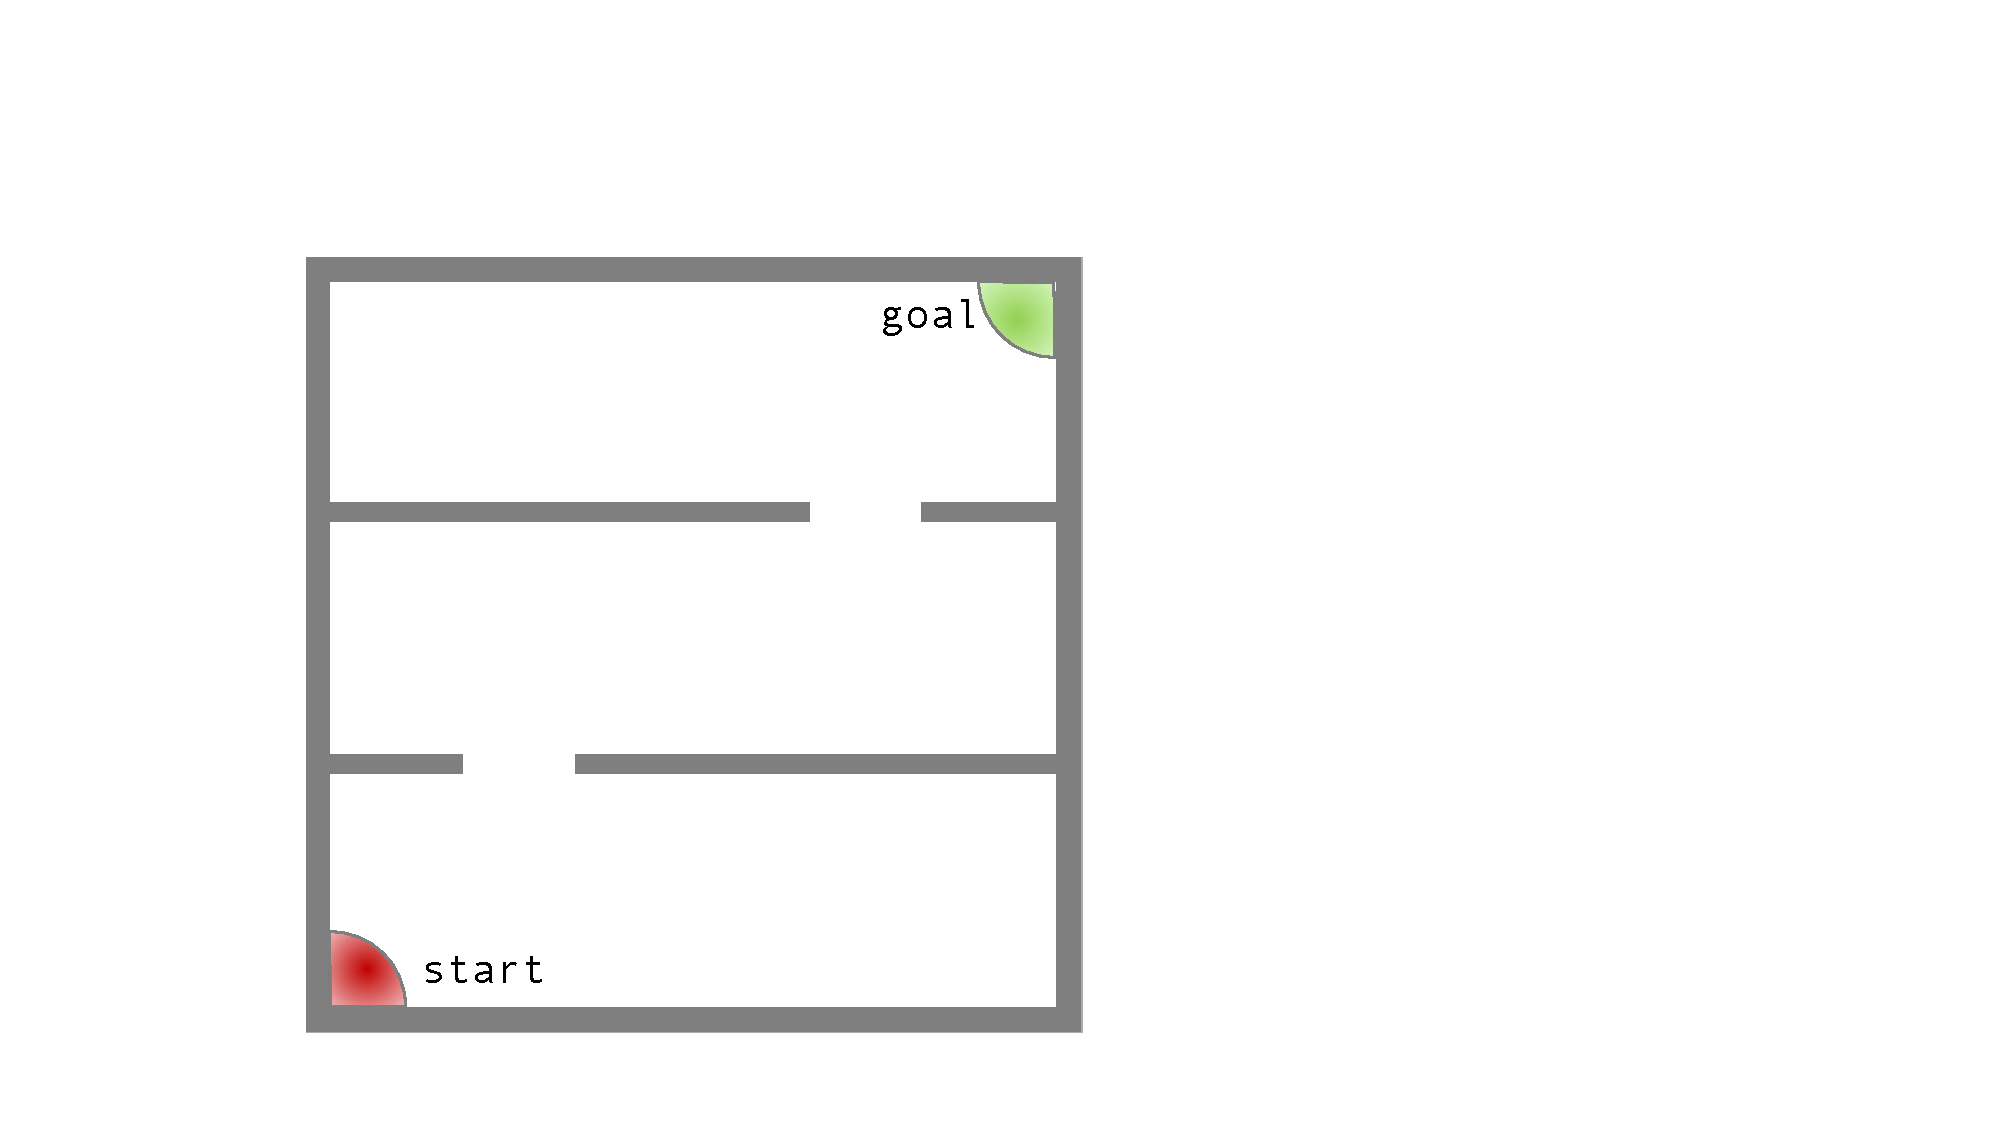
\includegraphics[trim=0.0cm 0.2cm 0.0cm 0.2cm,clip=true,height=2.6cm, width=2.0cm]{images/rooms2.pdf}
    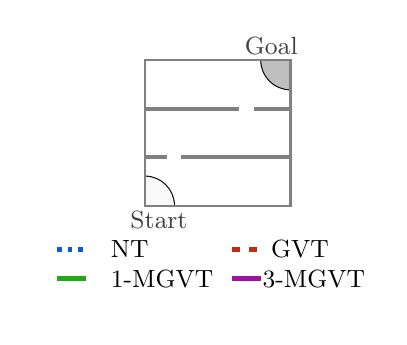
\begin{tikzpicture}[scale=0.37]
\draw [white] (0,0) grid (12,9);
%\begin{scope}[shift={(0,2)}]
%\draw [thick] (4,5) arc [radius=1, start angle=180, end angle= 270];
%\path [fill=gray!50, very thin] (4,5) arc [radius=1, start angle=180, end angle= 270] -- (5,4) --(5,5)--(4,5);
%\draw [thick] (0,1) arc [radius=1, start angle=90, end angle= 0];
%\path [fill=lightgray!10, very thin] (0,1) arc [radius=1, start angle=90, end angle=0] -- (1,0) --(0,0)--(0,1);
%
%%\draw [fill=black!50] (1,1) circle [radius=0.1cm];
%%\node at (1,1) [ right] {$A$};
%
%\node at (1.8,-0.5)[left] {\color{darkgray}\small Start};
%\node at (3.1,5.5) [right]{\color{darkgray}\small Goal};
%
%\draw [thick, gray] (0,0) rectangle (5,5);
%\draw [line width=0.5mm, gray] (1.25,5/3) -- (5,5/3);
%\draw [line width=0.5mm, gray] (0,5/3) -- (0.75,5/3);
%\draw [line width=0.5mm, gray] (0,10/3) -- (3.25,10/3);
%\draw [line width=0.5mm, gray] (3.75,10/3) -- (5,10/3);

%\draw [thick, line width=0.6mm, dotted, nt] (5.5,4) -- (7,4);
%\node at (7,4) [right] {NT};
%\draw [thick, line width=0.6mm, dashed,gvt] (5.5,3) -- (7,3);
%\node at (7,3) [right] {GVT};
%\draw [thick, line width=0.6mm, mgvt1] (5.5,2) -- (7,2);
%\node at (7,2) [right] {1-MGVT};
%\draw [thick, line width=0.6mm, mgvt3] (5.5,1) -- (7,1);
%\node at (7,1) [right] {3-MGVT};

\begin{scope}[shift={(0,3.8)}]
\begin{scope}[shift={(4,0)}]
\draw [thick] (4,5) arc [radius=1, start angle=180, end angle= 270];
\path [fill=gray!50, very thin] (4,5) arc [radius=1, start angle=180, end angle= 270] -- (5,4) --(5,5)--(4,5);
\draw [thick] (0,1) arc [radius=1, start angle=90, end angle= 0];
\path [fill=lightgray!10, very thin] (0,1) arc [radius=1, start angle=90, end angle=0] -- (1,0) --(0,0)--(0,1);

%\draw [fill=black!50] (1,1) circle [radius=0.1cm];
%\node at (1,1) [ right] {$A$};

\node at (1.8,-0.5)[left] {\color{darkgray}\small Start};
\node at (3.1,5.5) [right]{\color{darkgray}\small Goal};

\draw [thick, gray] (0,0) rectangle (5,5);
\draw [line width=0.5mm, gray] (1.25,5/3) -- (5,5/3);
\draw [line width=0.5mm, gray] (0,5/3) -- (0.75,5/3);
\draw [line width=0.5mm, gray] (0,10/3) -- (3.25,10/3);
\draw [line width=0.5mm, gray] (3.75,10/3) -- (5,10/3);

\end{scope}
\begin{scope}[shift={(1,0)}]
\draw [thick, line width=0.6mm, dotted, nt] (0,-1.5) -- (1,-1.5);
\node at (1.5,-1.5) [right] {\small NT};
\draw [thick, line width=0.6mm, dashed,gvt] (6, -1.5) -- (7,-1.5);
\node at (7,-1.5) [right] {\small GVT};
\draw [thick, line width=0.6mm, mgvt1] (0,-2.5) -- (1,-2.5);
\node at (1.5,-2.5) [right] {\small 1-MGVT};
\draw [thick, line width=0.6mm, mgvt3] (6, -2.5) -- (7,-2.5);
\node at (10.9,-2.5) [left] {\small 3-MGVT};
\end{scope}
\end{scope}
\end{tikzpicture} 
    %\caption{The rooms problem}\label{f:rooms}
  \end{subfigure}
  \begin{subfigure}[b]{0.32\textwidth}
    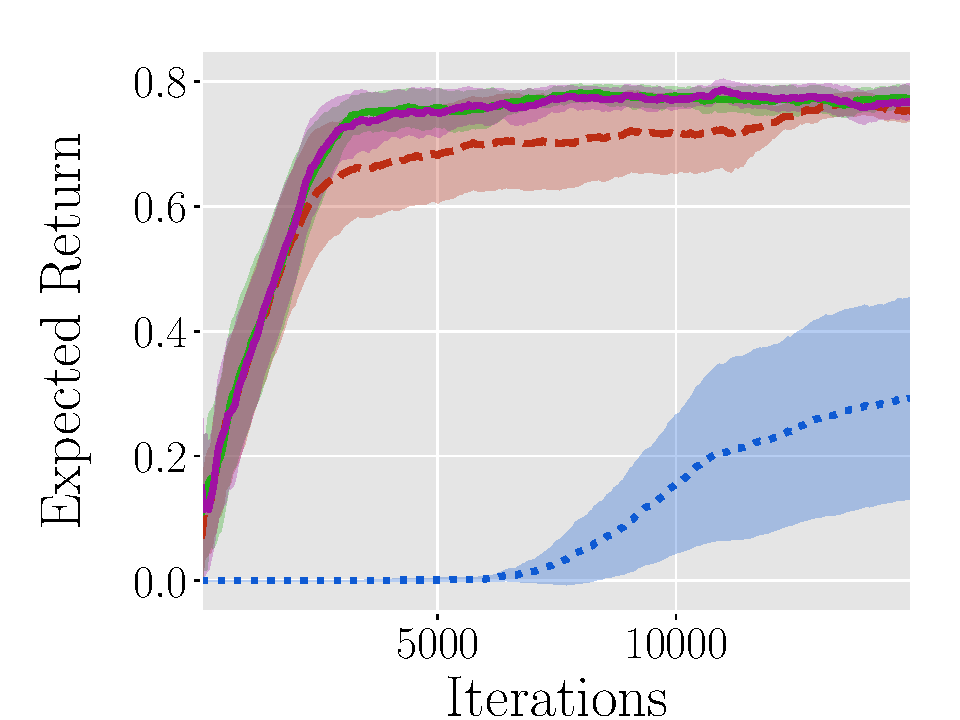
\includegraphics[trim=0cm 0cm 1.2cm 1.1cm,clip=true,height=2.9cm]{images/three-room/lrev.pdf}
    \caption{Rooms: two doors moving}\label{f:two_doors}
  \end{subfigure}
    \begin{subfigure}[b]{0.32\textwidth}
    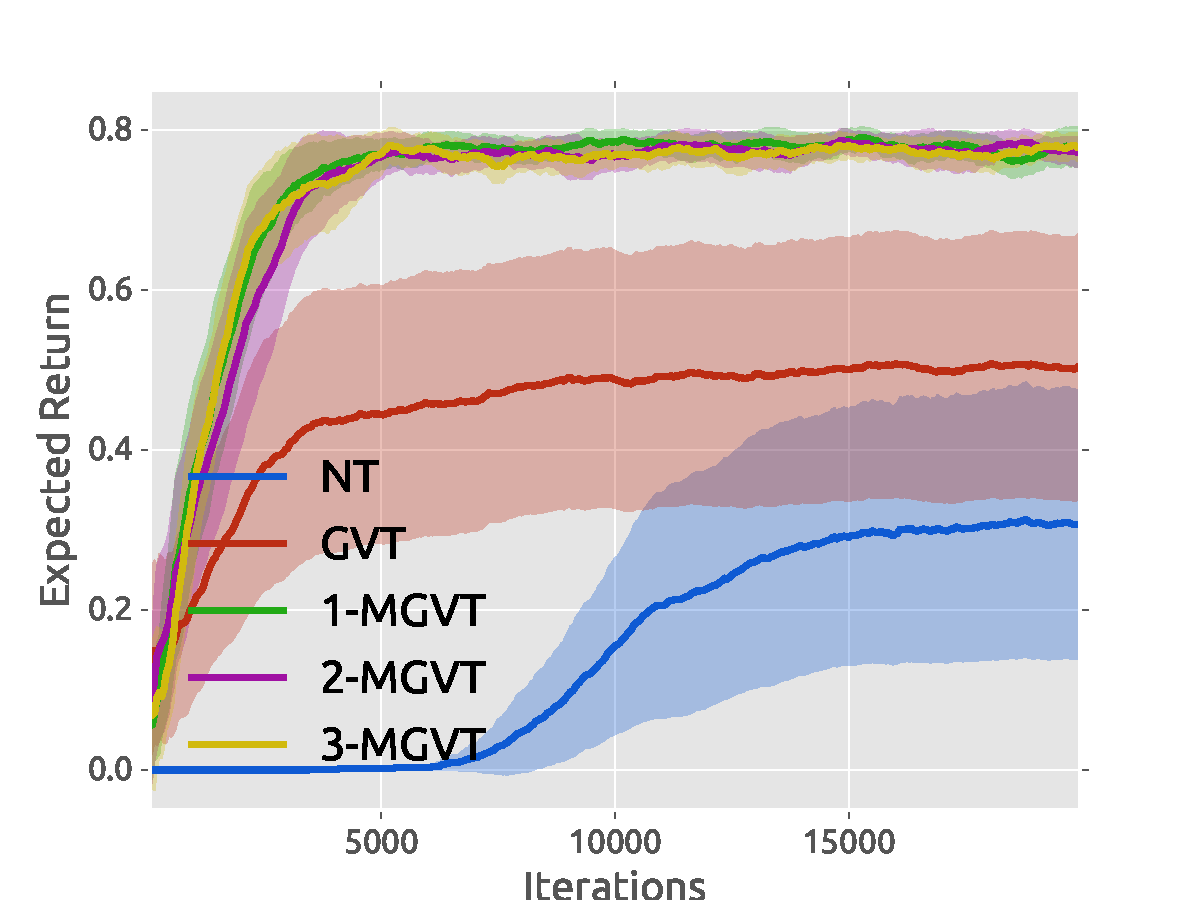
\includegraphics[trim=0cm 0cm 1.2cm 1.1cm,clip=true,height=2.9cm]{images/three-room-gen/lrev.pdf}
    \caption{Rooms: one door moving}\label{f:one_door}
  \end{subfigure}
%    \begin{subfigure}[b]{0.27\textwidth}
%    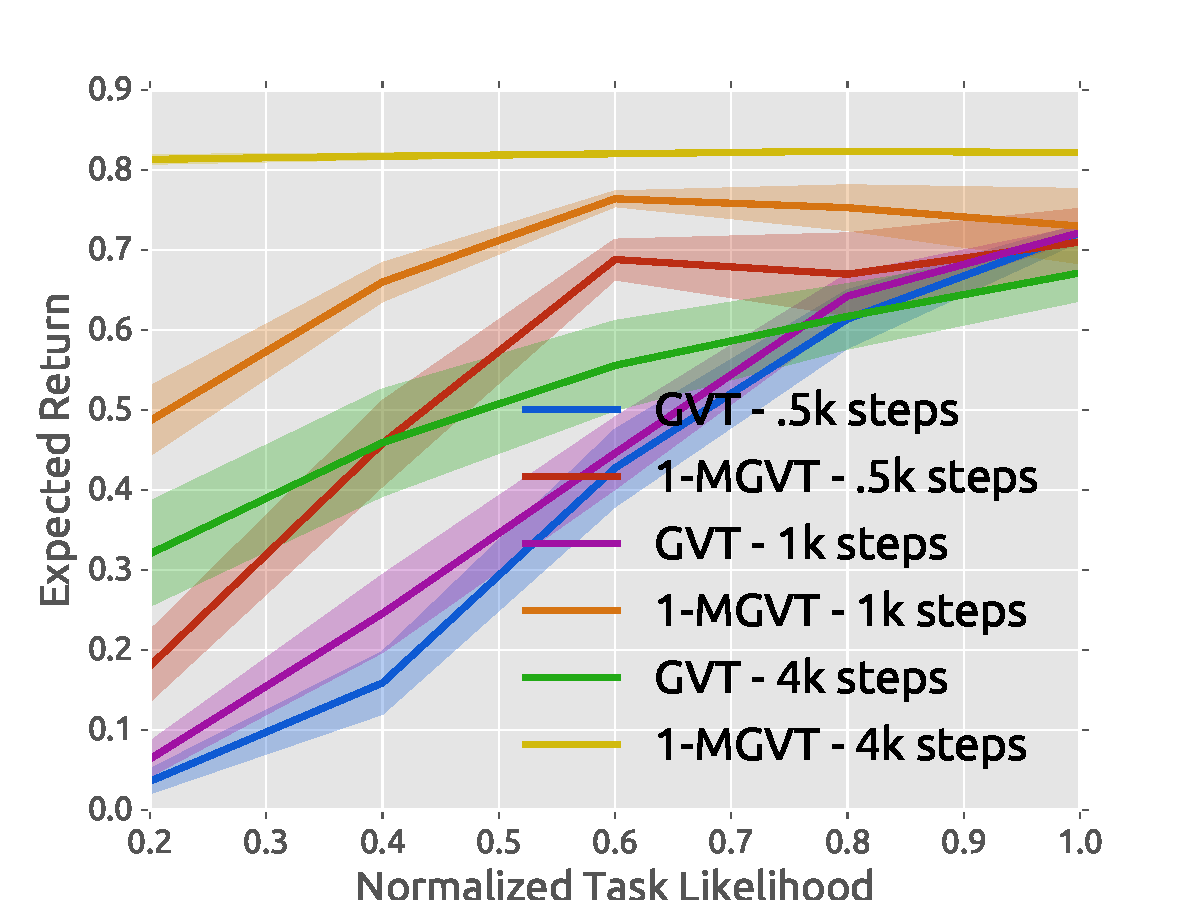
\includegraphics[trim=0cm 0cm 1.6cm 1.3cm,clip=true,height=2.9cm]{images/likelihood/lrew.pdf}
%    \caption{}\label{f:likelihood}
%  \end{subfigure}

	\begin{subfigure}[b]{0.32\textwidth}
    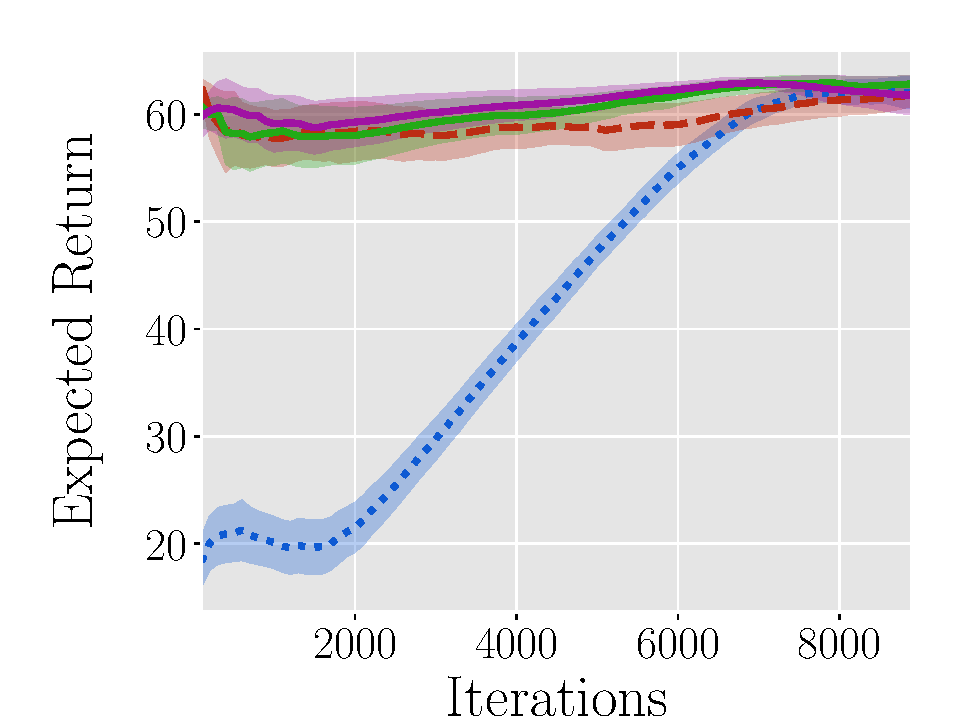
\includegraphics[trim=0.0cm 0cm 1.2cm 1.3cm,clip=true,height=2.9cm]{images/cartpole/lrev.pdf}
    \caption{Cartpole}\label{f:cartpole}
  \end{subfigure}
    \begin{subfigure}[b]{0.32\textwidth}
    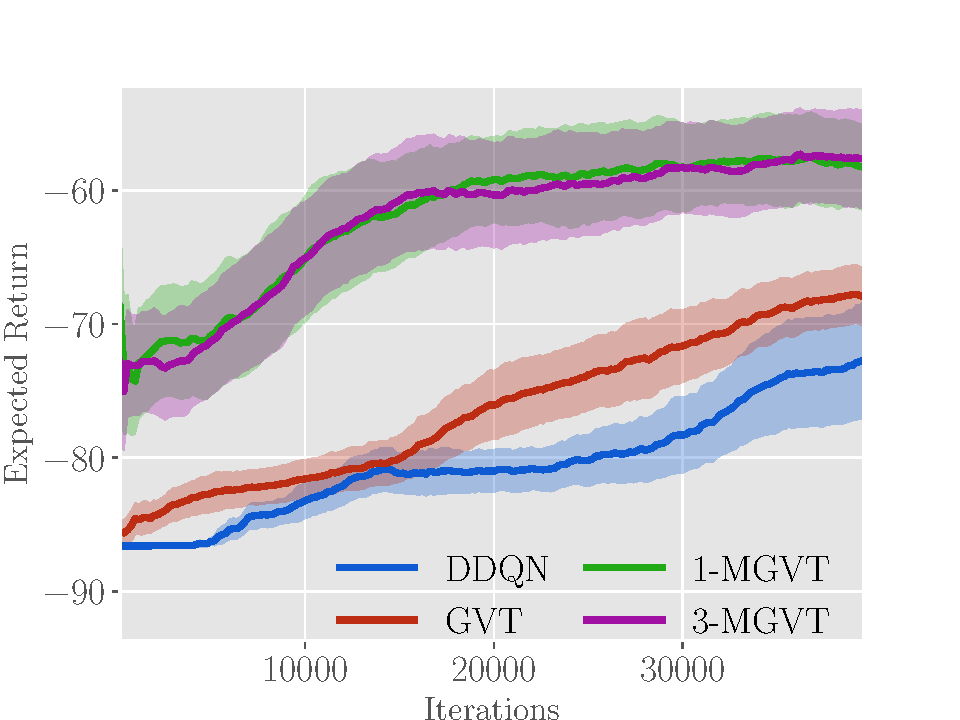
\includegraphics[trim=0.0cm 0cm 1.2cm 1.3cm,clip=true,height=2.9cm]{images/mountaincar/lrev.pdf}
    \caption{Mountain Car}\label{f:mountaincar}
  \end{subfigure}
    \begin{subfigure}[b]{0.32\textwidth}
    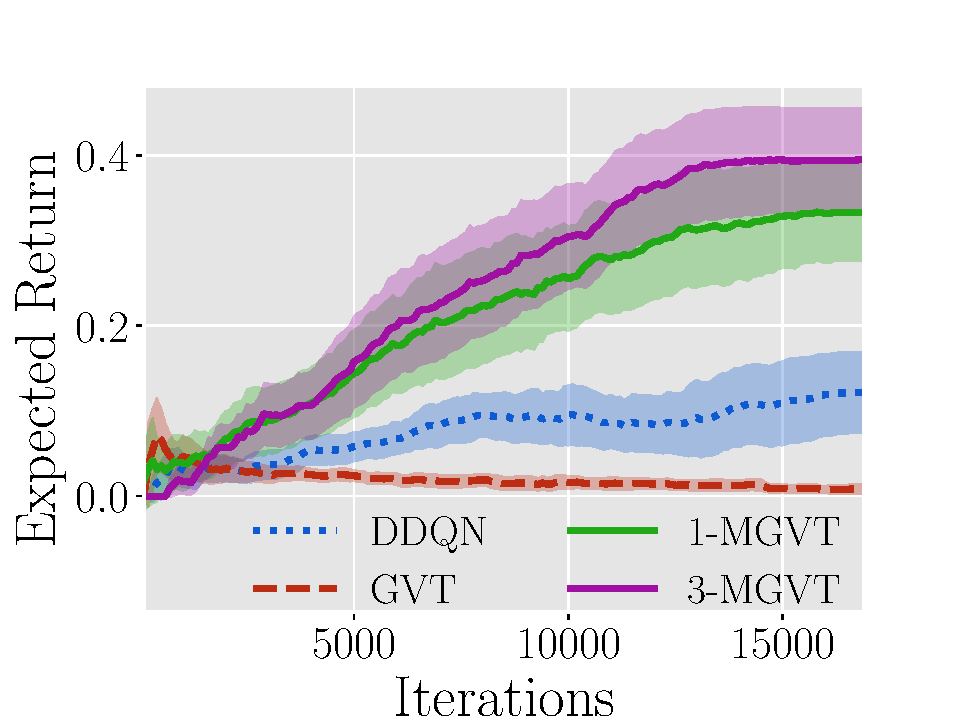
\includegraphics[trim=0.0cm 0cm 1.2cm 1.3cm,clip=true,height=2.9cm]{images/maze/lrev_main.pdf}
    \caption{Maze Navigation}\label{f:maze_results}
  \end{subfigure}
  \caption{Expected return as a function of the number of iterations averaged over $20$ independent runs. $95\%$ confidence intervals are shown.}
  \label{fig:main}
\end{figure*}
We consider an agent navigating in the environment depicted in Figure~\ref{fig:main}. The agent starts in the bottom-left corner and must move from one room to another to reach the goal position in the top-right corner. The rooms are connected by small doors whose locations are unknown to the agent. The state-space is modeled as a $10 \times 10$ continuous grid, while the action-space is the set of $4$ movement directions (up, right, down, left). After each action, the agent moves by $1$ in the chosen direction and the final position is corrupted by Gaussian noise $\mathcal{N}(0,0.2)$. In case the agent hits a wall, its position remains unchanged. The reward is $1$ when reaching the goal (after which the process terminates) and $0$ otherwise, while the discount factor is $\gamma = 0.99$. In this experiment, we consider linearly parameterized $Q$-functions with $121$ equally-spaced radial basis features.

We generate a set of $50$ source tasks for the three-room environment of Figure~\ref{fig:main} by sampling both door locations uniformly in the allowed space, and solve all of them by directly minimizing the TD error as presented in Section~\ref{sec:td}. Then, we use our algorithms to transfer from $10$ source tasks sampled from the previously generated set. The average return over the last $50$ learning episodes as a function of the number of iterations is shown in Figure~\ref{f:two_doors}. Each curve is the result of $20$ independent runs, each one resampling the target and source tasks, with $95\%$ confidence intervals. Further details on the parameters adopted in this experiment are given in Appendix \ref{app:c1}. As expected, the no-transfer (NT) algorithm fails at learning the task in so few iterations due to the limited exploration provided by an $\epsilon$-greedy policy. On the other hand, all our algorithms achieve a significant speed-up and converge to the optimal performance in few iterations, with GVT being slightly slower. Interestingly, we notice that there is no advantage in adopting more than $1$ component for the posterior in MGVT. This result is intuitive since, as soon as the algorithm figures out which is the target task, all the components move towards the same region.

To better understand the differences between GVT and MGVT, we now consider transferring from a slightly different distribution than the one from which target tasks are drawn. We generate $50$ source tasks again but this time with the bottom door fixed at the center and the other one moving. Then, we repeat the previous experiment, allowing both doors to move when sampling target tasks. The results are shown in Figure~\ref{f:one_door}. Interestingly, MGVT seems almost unaffected by this change, proving that it has sufficient representation power to generalize to slightly different task distributions. The same does not hold for GVT, which now is not able to solve many of the sampled target tasks, as can be noticed from the higher variance. This result proves again that assuming Gaussian distributions can pose severe limitations in our transfer settings.

\paragraph{Classic Control} \label{sec:cc}

We now consider two well-known classic control environments: Cartpole and Mountain Car \citep{sutton1998reinforcement}. For both, we generate $20$ source tasks by uniformly sampling their physical parameters (cart mass, pole mass, pole length for Cartpole and car speed for Mountain Car) and solve them by directly minimizing the TD error as in the previous experiment. We parameterize $Q$-functions using neural networks with one layer of $32$ hidden units for Cartpole and $64$ for Mountain Car. A better description of these two environments and their parameters is given in Appendix \ref{app:c2}. In this experiment, we use a Double Deep Q-Network (DDQN) \cite{van2016deep} to provide a stronger no-transfer baseline for comparison. The results (same settings of Section~\ref{sec:gw}) are shown in Figures~\ref{f:cartpole} and~\ref{f:mountaincar}. For Cartpole (Figure~\ref{f:cartpole}), all transfer algorithms are almost zero-shot. This result is expected since, although we vary the system parameters in a wide range, the optimal $Q$-values of states near the balanced position are similar for all tasks. On the contrary, in Mountain Car (Figure~\ref{f:mountaincar}) the optimal $Q$-functions become very different when changing the car speed. This phenomenon hinders the learning of GVT in the target task, while MGVT achieves a good jump-start and converges in fewer iterations.

\paragraph{Maze Navigation} \label{sec:mn}

%\begin{figure*}[t]
%  \begin{subfigure}[b]{0.32\textwidth}
%    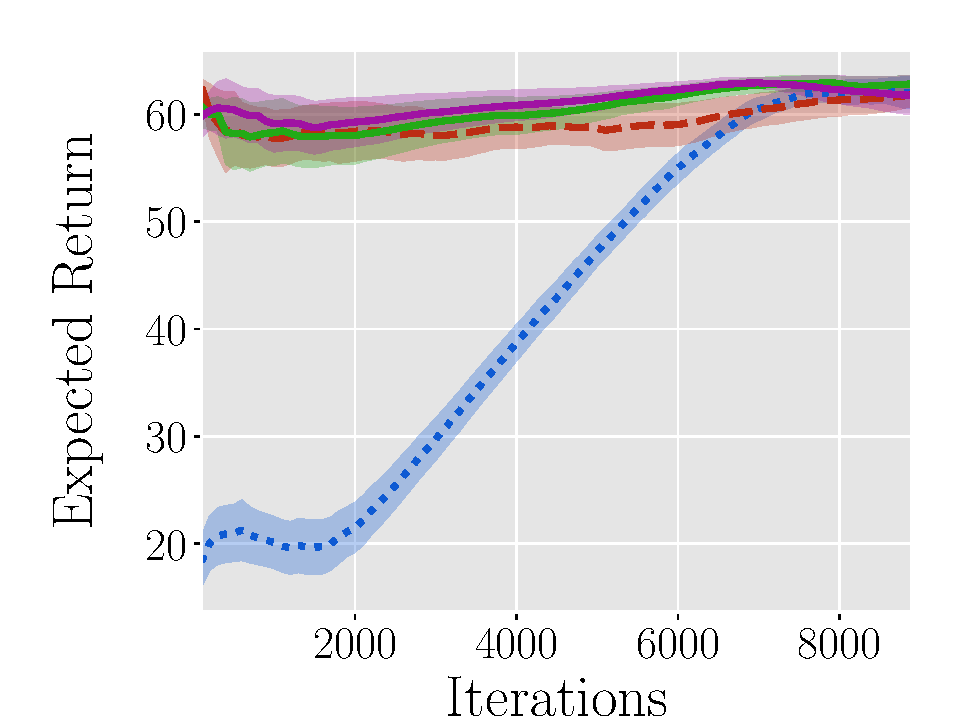
\includegraphics[trim=0.0cm 0cm 1.8cm 1.3cm,clip=true,height=2.9cm]{images/cartpole/lrev.pdf}
%    \caption{}\label{f:cartpole}
%  \end{subfigure}
%    \begin{subfigure}[b]{0.32\textwidth}
%    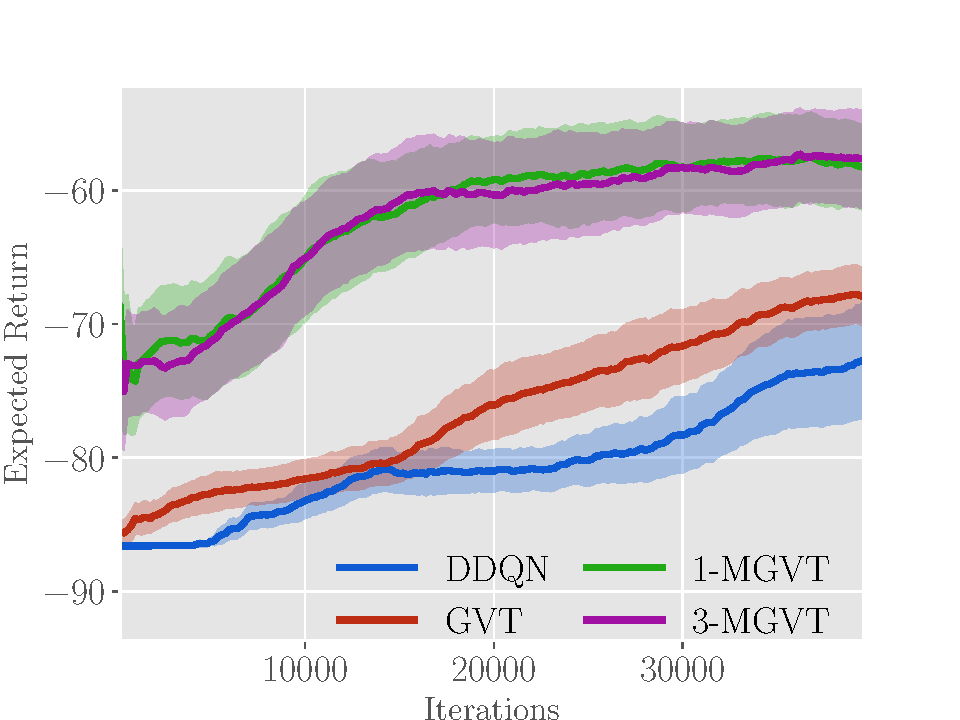
\includegraphics[trim=0.0cm 0cm 1.6cm 1.3cm,clip=true,height=2.9cm]{images/mountaincar/lrev.pdf}
%    \caption{}\label{f:mountaincar}
%  \end{subfigure}
%    \begin{subfigure}[b]{0.32\textwidth}
%    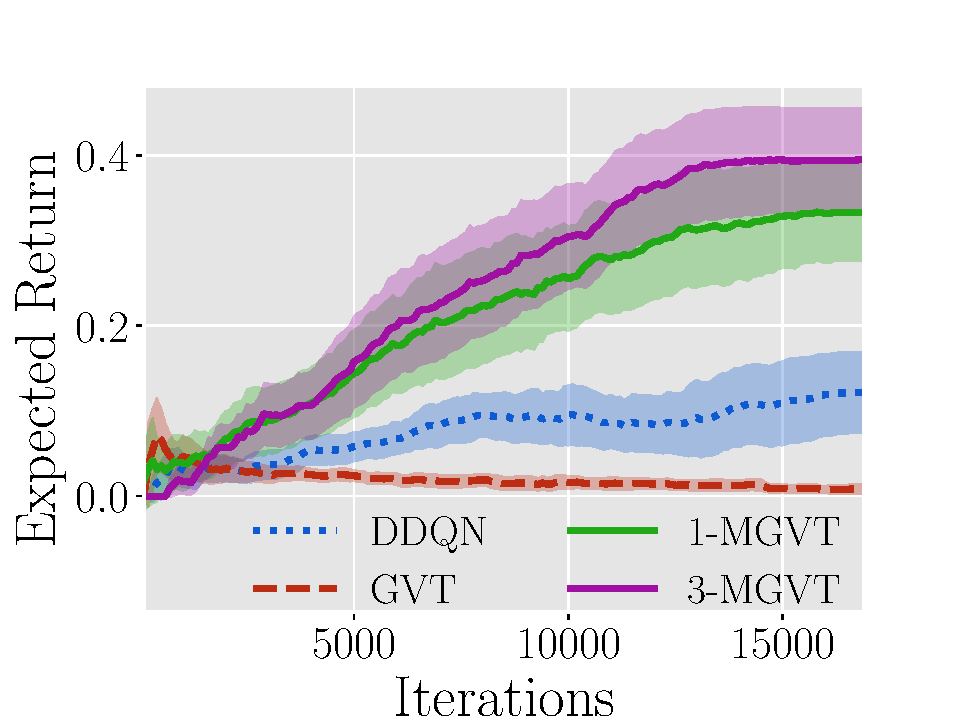
\includegraphics[trim=0.0cm 0cm 1.6cm 1.3cm,clip=true,height=2.9cm]{images/maze/lrev_main.pdf}
%    \caption{}\label{f:maze_results}
%  \end{subfigure}
%  \caption{(a) Cartpole, (b) Mountain Car, and (c) Maze Navigation}
%  \label{fig:ccmazeplots}
%\end{figure*}

In our last experiment, we consider a robotic agent navigating mazes. At the beginning of each episode, the agent is dropped to a random position in a $10m^2$ maze and must reach a goal area in the smallest time possible. The robot is equipped with sensors detecting its absolute position, its orientation, the distance to any obstacle within $2m$ in $9$ equally-spaced directions, and whether the goal is present in the same range. The only actions available are \textit{move forward} with speed $0.5m/s$ or \textit{rotate} (in either direction) with speed of $\pi/8\ rad/s$. Each time step corresponds to $1s$ of simulation. The reward is $1$ for reaching the goal and $0$ otherwise, while the discount factor is $\gamma=0.99$. For this experiment, we design a set of $20$ different mazes and solve them using a DDQN with two layers of $32$ neurons and ReLU activations. Then, we fix a target maze and transfer from $5$ source mazes uniformly sampled from such set (excluding the chosen target). To further assess the robustness of our method, we now consider transferring from the $Q$-functions learned by DDQNs instead of those obtained by minimizing the TD error as in the previous domains. From our considerations of Sections~\ref{sec:td} and~\ref{sec:theory}, the fixed-points of the two algorithms are different, which creates a further challenge for our method. We show the results for a fixed target maze in Figure~\ref{f:maze_results}, while referring the reader to Appendix  \ref{app:c3} for the illustration of our mazes and additional results. Once again, MGVT achieves a remarkable speed-up over (no-transfer) DDQN. This time, using $3$ components achieves slightly better performance than using only $1$, which is likely due to the fact that the task distribution is much more complicated than in the previous domains. For the same reason, GVT shows negative transfer and performs even worse than DDQN.

\section{Related Works}

Our approach is mostly related to \cite{lazaric2010bayesian}. Although we both assume the tasks to share similarities in their value functions, \cite{lazaric2010bayesian} consider only linear approximators and adopt a hierarchical Bayesian model of the corresponding weights' distribution, which is assumed Gaussian. On the other hand, our variational approximation allows for more general distribution families and can be combined with non-linear approximators. Furthermore, \cite{lazaric2010bayesian} propose a Dirichlet process model for the case where weights cluster into different classes, which relates to our mixture formulation and proves the importance of capturing more complicated task distributions again. Finally, \cite{lazaric2010bayesian} considers the problem of jointly learning all given tasks, while we focus on transferring information from a set of source tasks to the target task. In \cite{wilson2007multi}, the authors propose a hierarchical Bayesian model for the distribution over MDPs. Unlike our approach and \cite{lazaric2010bayesian}, they consider a distribution over transition probabilities and rewards, rather than value functions. In the same spirit of our method, they consider a Thompson sampling-based procedure which, at each iteration, samples a new task from the posterior and solves it. However, \cite{wilson2007multi} consider only finite MDPs, which poses a severe limitation on the algorithm's applicability. On the contrary, our approach can handle high-dimensional tasks. In \cite{doshi2016hidden}, the authors consider a family of tasks whose dynamics are governed by some hidden parameters and use Gaussian processes (GPs) to model such dynamics across tasks. Recently, \cite{killian2017robust} extended this approach by replacing GPs with Bayesian neural networks to obtain a more scalable approach. Both approaches result in a model-based algorithm that quickly adapts to new tasks by estimating their hidden parameters, while we propose a model-free method which does not require such assumptions.

%In RL, our approach is related to value function randomization\cite{osband2014generalization}, which extends the well-known LSTD \cite{boyan1999least} by adopting Bayesian linear regression to model the uncertainty over the predicted value function weights, and use that to perform a form of Thompson sampling. Such approach was recently extended by \cite{azizzadenesheli2018efficient}, where the approximator is replaced by a Bayesian neural network, leading to an algorithm capable of solving much more complicated problems. Both these algorithms rely on the Gaussian assumption and, since they work in plain RL settings, have no informative prior available. On the other hand, our variational approximation allows more complex distributions (e.g., mixtures) to be adopted, while knowledge from the source tasks allows us to learn very informative priors.

\section{Conclusion}

We presented a variational method for transferring value functions in RL. We showed our approach to be general, in the sense that it can be combined with several distributions and function approximators, while providing two practical algorithms based on Gaussians and mixtures of Gaussians, respectively. We analyzed both from a theoretical and empirical perspectives, proving that the Gaussian version has severe limitations, while the mixture one is much better for our transfer settings. We evaluated the proposed algorithms in different domains, showing that both achieve excellent performance in simple tasks, while only the mixture version is able to handle complex environments.

Since our algorithm effectively models the uncertainty over tasks, a relevant future work is to design an algorithm that explicitly explores the target task to reduce such uncertainty (e.g., \cite{houthooft2016vime}). Furthermore, our variational approach could be extended to model a distribution over optimal policies instead of value functions (e.g., \cite{sehnke2008policy,liu2017stein}), which might allow better transferred behavior.

{\small 
\bibliography{biblio.bib}
\bibliographystyle{plain}
}

\newpage
\appendix

\section{Proofs}

\subsection{Proof of Theorem 1}\label{app:a1}

\thmm*
\begin{proof}
We begin by noticing that:
\begin{align*}
\norm{Q^*-\wt{Q}}_{\infty} =\ & \norm{TQ^* - \wt{T}\wt{Q}}_{\infty} \\ =\ &
\norm{TQ^* - \wt{T}Q^* + \wt{T}Q^* - \wt{T}\wt{Q}}_{\infty} \\ \leq\ &
\norm{TQ^* - \wt{T}Q^*}_{\infty} + \norm{\wt{T}Q^* - \wt{T}\wt{Q}}_{\infty} \\ \leq\ &
\norm{TQ^* - \wt{T}Q^*}_{\infty} + \gamma\norm{Q^* - \wt{Q}}_{\infty},
\end{align*}
where the first inequality follows from Minkowsky's inequality and the second one from the contraction property of the mellow Bellman operator. This implies that:
\begin{align} \label{eq:mm1}
\norm{Q^*-\wt{Q}}_{\infty} \leq \frac{1}{1-\gamma}\norm{TQ^* - \wt{T}Q^*}_{\infty}.
\end{align}
Let us bound the norm on the right-hand side separately. In order to do that, we will bound the function $\abs{TQ^*(s,a) - \wt{T}Q^*(s,a)}$ point-wisely for any pair $\langle s,a\rangle$. By applying the definition of the optimal and mellow Bellman operators, we obtain:
\begin{align} \label{eq:mm5}
\abs{TQ^*(s,a) - \wt{T}Q^*(s,a)} =\ & \abs{R(s,a) + \gamma\mathbb{E}\left[\max_{a'}Q^*(s',a')\right] - R(s,a) - \gamma\mathbb{E}\left[\mm_{a'}Q^*(s',a')\right]}\notag \\ =\ & \gamma\abs{\mathbb{E}\left[\max_{a'}Q^*(s',a')\right] - \mathbb{E}\left[\mm_{a'}Q^*(s',a')\right]}\notag \\ \leq\ & \gamma\mathbb{E}\left[\abs{\max_{a'}Q^*(s',a') - \mm_{a'}Q^*(s',a')}\right].
\end{align}
Thus, bounding this quantity reduces to bounding $\abs{\max_{a}Q^*(s,a) - \mm_{a}Q^*(s,a)}$ point-wisely for any $s$. Recall that applying the mellow Bellman operator is equivalent to computing an expectation under a Boltzmann distribution with inverse temperature $\beta_{\kappa}$ induced by $\kappa$ \cite{asadi2017alternative}. Thus, we can write:
\begin{align} \label{eq:mm2}
\abs{\max_a Q^*(s,a) - \mm_a Q^*(s,a)} =\ & \abs{\sum_a \pi^*(a|s)Q^*(s,a) - \sum_a \pi_{\beta_{\kappa}}(a|s)Q^*(s,a)}\notag\\ =\ & \abs{\sum_a Q^*(s,a) \left( \pi^*(a|s) - \pi_{\beta_{\kappa}}(a|s)  \right)}\notag\\ \leq\ & \sum_a \abs{Q^*(s,a)} \abs{\pi^*(a|s) - \pi_{\beta_{\kappa}}(a|s)}\notag\\ \leq\ & \frac{R_{max}}{1-\gamma}\sum_a\abs{\pi^*(a|s) - \pi_{\beta_{\kappa}}(a|s)},
\end{align}
where $\pi^*$ is the optimal (deterministic) policy w.r.t. $Q^*$ and $\pi_{\beta_{\kappa}}$ is the Boltzmann distribution induced by $Q^*$ with inverse temperature $\beta_{\kappa}$:
\begin{align*}
\pi_{\beta_{\kappa}}(a|s) = \frac{e^{\beta_{\kappa} Q^*(s,a)}}{\sum_{a'}e^{\beta_{\kappa} Q^*(s,a')}}.
\end{align*}
Denote by $a_1(s)$ the optimal action for state $s$ under $Q^*$. We can then write:
\begin{align} \label{eq:mm3}
\sum_a\abs{\pi^*(a|s) - \pi_{\beta_{\kappa}}(a|s)} =\ & \abs{\pi^*(a_1(s)|s) - \pi_{\beta_{\kappa}}(a_1(s)|s)} + \sum_{a \neq a_1(s)}\abs{\pi^*(a|s) - \pi_{\beta_{\kappa}}(a|s)}\notag\\ =\ & \abs{1 - \pi_{\beta_{\kappa}}(a_1(s)|s)} + \sum_{a \neq a_1(s)}\abs{\pi_{\beta_{\kappa}}(a|s)}\notag\\ =\ & 2\abs{1 - \pi_{\beta_{\kappa}}(a_1(s)|s)}.
\end{align}
Finally, denoting with $a_2(s)$ the second-best action in state $s$, let us bound this last term:
\begin{align} \label{eq:mm4}
\abs{1 - \pi_{\beta_{\kappa}}(a_1(s)|s)} =\ & \abs{1 - \frac{e^{\beta_{\kappa} Q^*(s,a_1(s))}}{\sum_{a'}e^{\beta_{\kappa} Q^*(s,a')}}}\notag\\ =\ & \abs{1 - \frac{e^{\beta_{\kappa} \left( Q^*(s,a_1(s)) - Q^*(s,a_2(s)) \right)}}{\sum_{a'}e^{\beta_{\kappa} \left( Q^*(s,a') - Q^*(s,a_2(s))\right)}}}\notag\\ =\ & \abs{1 - \frac{e^{\beta_{\kappa} g(s)}}{\sum_{a'}e^{\beta_{\kappa} \left( Q^*(s,a') - Q^*(s,a_2(s))\right)}}}\notag\\ =\ & \abs{1 - \frac{e^{\beta_{\kappa} g(s)}}{e^{\beta_{\kappa} g(s)} + \sum_{a' \neq a_1(s)}e^{\beta_{\kappa} \left( Q^*(s,a') - Q^*(s,a_2(s))\right)}}}\notag\\ \leq & \abs{1 - \frac{e^{\beta_{\kappa} g(s)}}{e^{\beta_{\kappa} g(s)} + \abs{\mathcal{A}}}}\notag\\ = & \abs{\frac{1}{1 + \frac{1}{\abs{\mathcal{A}}}e^{\beta_{\kappa} g(s)}}}.
\end{align}
Combining Eq. \eqref{eq:mm2}, \eqref{eq:mm3}, and \eqref{eq:mm4}, we obtain:
\begin{align*}
\abs{\max_a Q(s,a) - \mm_a Q(s,a)} \leq\ \frac{2 R_{max}}{1-\gamma}\abs{\frac{1}{1 + \frac{1}{\abs{\mathcal{A}}}e^{\beta_{\kappa} g(s)}}}.
\end{align*}
Finally, using Eq. \eqref{eq:mm5} we get:
\begin{align*}
\abs{TQ^*(s,a) - \wt{T}Q^*(s,a)} \leq \frac{2\gamma R_{max}}{1-\gamma}\abs{\frac{1}{1 + \frac{1}{\abs{\mathcal{A}}}e^{\beta_{\kappa} g(s)}}}.
\end{align*}
Taking the norm and plugging this into Eq. \eqref{eq:mm1} concludes the proof.
\end{proof}

\subsection{Proof of Theorem 2}\label{app:a2}

We begin by proving some important lemmas. Then, we use them to derive a finite-sample analysis of Algorithm~\ref{alg:transfer} with linearly parameterized value functions for both Gaussian distributions (Theorem \ref{th:main-gaussian}) and Gaussian mixture models (Theorem \ref{th:main-mixture}). We start by proving some important properties of the variational approximation introduced in Section~\ref{sec:alg}. Our results generalize those of existing works that consider variational approximations of intractable Gibbs posteriors \cite{alquier2016properties,cottet20181}. From now on, we consider only $Q$-functions parameterized by weights $\bm{w}$ and assume them to be uniformly bounded by $\frac{R_{max}}{1-\gamma}$. 

\begin{lemma}\label{lemma:l2}
Let $p$ and $q$ be arbitrary distributions over weights $\bm{w}$, and $\nu$ be a probability measure over $\mathcal{S}\times\mathcal{A}$. Consider a dataset $D$ of $N$ i.i.d. samples where state-action couples are distributed according to $\nu$ and define $\text{v}(\bm{w}) \triangleq \mathbb{E}_{\nu}\left[Var_{\mathcal{P}}\left[\wt b(\bm{w})\right]\right]$. Then, for any $\lambda > 0$ and $\delta > 0$, with probability at least $1-\delta$, the following two inequalities hold simultaneously:
\begin{equation}\label{eq:lemma2-1}
\mathbb{E}_q\left[ \norm{\wt B_{\bm{w}}}_{\nu}^2 \right ] \leq \mathbb{E}_q\left[ \norm{\wt B_{\bm{w}}}_D^2 \right] - \mathbb{E}_q\left[ \text{v}(\bm{w}) \right] + \frac{\lambda}{N} KL(q||p) + 4\frac{R_{max}^2}{(1-\gamma)^2}\sqrt{\frac{\log\frac{2}{\delta}}{2N}}
\end{equation}
\begin{equation}\label{eq:lemma2-2}
\mathbb{E}_q\left[ \norm{\wt B_{\bm{w}}}_D^2 \right] \leq \mathbb{E}_q\left[ \norm{\wt B_{\bm{w}}}_{\nu}^2 \right ] + \mathbb{E}_q\left[ \text{v}(\bm{w}) \right] + \frac{\lambda}{N} KL(q||p) + 4\frac{R_{max}^2}{(1-\gamma)^2}\sqrt{\frac{\log\frac{2}{\delta}}{2N}}.
\end{equation}
\end{lemma}
\begin{proof}
From Hoeffding's inequality we have:
\begin{align*}
P\left( \abs{\mathbb{E}_{\nu,\mathcal{P}}\left[\norm{\wt B_{\bm{w}}}_D^2\right] - \norm{\wt B_{\bm{w}}}_D^2} > \epsilon \right) \leq 2\exp\left( -\frac{2N\epsilon^2}{\left(2\frac{R_{max}}{1-\gamma}\right)^4} \right)
\end{align*}
which implies that, for any $\delta>0$, with probability at least $1-\delta$:
\begin{align*}
\abs{\mathbb{E}_{\nu,\mathcal{P}}\left[\norm{\wt B_{\bm{w}}}_D^2\right] - \norm{\wt B_{\bm{w}}}_D^2} \leq 4\frac{R_{max}^2}{(1-\gamma)^2}\sqrt{\frac{\log\frac{2}{\delta}}{2N}}.
\end{align*}
Under independence assumptions, the expected TD error can be re-written as:
\begin{align*}
\mathbb{E}_{\nu,\mathcal{P}}\left[\norm{\wt B_{\bm{w}}}_D^2\right] =\ & \mathbb{E}_{\nu,\mathcal{P}}\left[\frac{1}{N}\sum_{i=1}^N (r_i + \gamma \mm_{a'} Q_{\bm{w}}(s_i',a') - Q_{\bm{w}}(s_i,a_i))^2\right]\\ =\ & \mathbb{E}_{\nu,\mathcal{P}}\left[(R(s,a) + \gamma \mm_{a'} Q_{\bm{w}}(s',a') - Q_{\bm{w}}(s,a))^2\right]\\ =\ & \mathbb{E}_{\nu}\left[\mathbb{E}_{\mathcal{P}}\left[\wt b(\bm{w})^2\right]\right]\\ =\ & \mathbb{E}_{\nu}\left[Var_{\mathcal{P}}\left[\wt b(\bm{w})\right] + \mathbb{E}_{\mathcal{P}}\left[\wt b(\bm{w})\right]^2\right]\\ =\ & v(\bm{w}) + \norm{\wt B_{\bm{w}}}_{\nu}^2,
\end{align*}
where $v(\bm{w}) \triangleq \mathbb{E}_{\nu}\left[Var_{\mathcal{P}}\left[\wt b(\bm{w})\right]\right]$. Thus:
\begin{align}\label{eq:hoeff}
\abs{\norm{\wt B_{\bm{w}}}_{\nu}^2 + v(\bm{w}) - \norm{\wt B_{\bm{w}}}_D^2} \leq 4\frac{R_{max}^2}{(1-\gamma)^2}\sqrt{\frac{\log\frac{2}{\delta}}{2N}}.
\end{align}
From the change of measure inequality \cite{seldin2012pac}, we have that, for any measurable function $f(\bm{w})$ and any two probability measures $p$ and $q$:
\begin{align*}
\log\mathbb{E}_p\left[e^{f(\bm{w})}\right] \geq \mathbb{E}_q\left[ f(\bm{w}) \right] - KL(q||p).
\end{align*}
Thus, multiplying both sides of \eqref{eq:hoeff} by $\lambda^{-1}N$ and applying the change of measure inequality with $f(\bm{w}) = \lambda^{-1}N\abs{\norm{\wt B_{\bm{w}}}_{\nu}^2 + v(\bm{w}) - \norm{\wt B_{\bm{w}}}_D^2}$, we obtain:
\begin{align*}
\mathbb{E}_q\left[ f(\bm{w}) \right] - KL(q||p) \leq \log\mathbb{E}_p\left[e^{f(\bm{w})}\right] \leq 4\frac{R_{max}^2 \lambda^{-1}N}{(1-\gamma)^2}\sqrt{\frac{\log\frac{2}{\delta}}{2N}},
\end{align*}
where the second inequality holds since the right-hand side of \eqref{eq:hoeff} does not depend on $\bm{w}$. Finally, we can explicitly write:
\begin{align*}
\mathbb{E}_q\left[ \abs{\norm{\wt B_{\bm{w}}}_{\nu}^2 + v(\bm{w}) - \norm{\wt B_{\bm{w}}}_D^2} \right] \leq \frac{\lambda}{N} KL(q||p) + 4\frac{R_{max}^2}{(1-\gamma)^2}\sqrt{\frac{\log\frac{2}{\delta}}{2N}}
\end{align*}
from which the lemma follows straightforwardly.
\end{proof}

From Lemma \ref{lemma:l2} we can straightforwardly prove the following result which will be of fundamental importance in the remaining.

\begin{lemma}\label{lemma:general-bound}
Fix a task $\mathcal{M}_{\tau}$. Let $p$ be a prior distribution over weights $\bm{w}$, and $\nu$ be a probability measure over $\mathcal{S}\times\mathcal{A}$. Assume $\wh{\xi}$ is the minimizer of \eqref{eq:elbo} for a dataset $D$ of $N$ i.i.d. samples where state-action couples are distributed according to $\nu$. Define $\text{v}(\bm{w}) \triangleq \mathbb{E}_{\nu}\left[Var_{\mathcal{P}_{\tau}}\left[\wt b(\bm{w})\right]\right]$. Then, for any $\delta > 0$, with probability at least $1-\delta$:
\begin{align*}
\mathbb{E}_{q_{\wh{\xi}}}\left[ \norm{\wt B_{\bm{w}}}_{\nu}^2 \right ] \leq \inf_{\xi \in \Xi}\left\{ \mathbb{E}_{q_{\xi}}\left[ \norm{\wt B_{\bm{w}}}_{\nu}^2 \right ] + \mathbb{E}_{q_{\xi}}\left[ v(\bm{w}) \right] + 2\frac{\lambda}{N} KL({q_{\xi}}||p) \right\} + 8\frac{R_{max}^2}{(1-\gamma)^2}\sqrt{\frac{\log\frac{2}{\delta}}{2N}}.
\end{align*}
\end{lemma}
\begin{proof}
Let us use Lemma \ref{lemma:l2} for the specific choice $q=q_{\wh{\xi}}$. From Eq. \eqref{eq:lemma2-1}, we have:
\begin{align*}
\mathbb{E}_{q_{\wh{\xi}}}\left[ \norm{\wt B_{\bm{w}}}_{\nu}^2 \right ] \leq\ & \mathbb{E}_{q_{\wh{\xi}}}\left[ \norm{\wt B_{\bm{w}}}_D^2 \right] - \mathbb{E}_{q_{\wh{\xi}}}\left[ v(\bm{w}) \right] + \frac{\lambda}{N} KL({q_{\wh{\xi}}}||p) + 4\frac{R_{max}^2}{(1-\gamma)^2}\sqrt{\frac{\log\frac{2}{\delta}}{2N}}\\ \leq\ & \mathbb{E}_{q_{\wh{\xi}}}\left[ \norm{\wt B_{\bm{w}}}_D^2 \right] + \frac{\lambda}{N} KL({q_{\wh{\xi}}}||p) + 4\frac{R_{max}^2}{(1-\gamma)^2}\sqrt{\frac{\log\frac{2}{\delta}}{2N}}\\ =\ & \inf_{\xi \in \Xi}\left\{ \mathbb{E}_{q_{\xi}}\left[ \norm{\wt B_{\bm{w}}}_D^2 \right] + \frac{\lambda}{N} KL({q_{\xi}}||p) \right\} + 4\frac{R_{max}^2}{(1-\gamma)^2}\sqrt{\frac{\log\frac{2}{\delta}}{2N}},
\end{align*}
where the second inequality holds since $v(\bm{w}) > 0$, while the equality holds from the definition of $\wh{\xi}$. We can now use Eq. \eqref{eq:lemma2-2} to bound $\mathbb{E}_{q_{\xi}}\left[ \norm{\wt B_{\bm{w}}}_D^2 \right]$, thus obtaining:
\begin{align*}
\mathbb{E}_{q_{\wh{\xi}}}\left[ \norm{\wt B_{\bm{w}}}_{\nu}^2 \right ] \leq \inf_{\xi \in \Xi}\left\{ \mathbb{E}_{q_{\xi}}\left[ \norm{\wt B_{\bm{w}}}_{\nu}^2 \right ] + \mathbb{E}_{q_{\xi}}\left[ v(\bm{w}) \right] + 2\frac{\lambda}{N} KL({q_{\xi}}||p) \right\} + 8\frac{R_{max}^2}{(1-\gamma)^2}\sqrt{\frac{\log\frac{2}{\delta}}{2N}}.
\end{align*}
This concludes the proof.
\end{proof}

It is worth noting the generality of Lemma \ref{lemma:general-bound}: in bounding the expected Bellman error we do not need to assume any particular distribution, nor we have to assume any particular function approximator.

We are now ready to state our main result. We start from the Gaussian case and then straightforwardly extend the proof to the mixture one.

\begin{restatable}{theorem}{thg} \label{th:main-gaussian}
Fix a target task $\mathcal{M}_{\tau}$. Assume linearly parameterized value functions $Q_{\bm{w}}(s,a)=\bm{w}^T\bm{\phi}(s,a)$ with bounded weights $\norm{\bm{w}}_{2}\leq w_{max}$ and uniformly bounded features $\norm{\bm{\phi}(s,a)}_{2}\leq \phi_{\max}$. Consider the Gaussian version of Algorithm~\ref{alg:transfer} with prior $p(\bm{w}) =\mathcal{N}(\bm{\mu}_p,\bm{\Sigma}_p)$ and denote by $(\wh{\bm{\mu}},\wh{\bm{\Sigma}})$ the variational parameter minimizing the objective of Eq.~\eqref{eq:elbo} on a dataset $D$ of $N$ i.i.d. samples distributed according to $\tau$ and $\nu$. Let $\bm{w}^* = \arginf_{\bm{w}}\norm{\wt{B}_{\bm{w}}}_{\nu}^2$ and define $\upsilon(\bm{w}^*) \triangleq \mathbb{E}_{\mathcal{N}(\bm{w}^*,\frac{1}{N}\bm{I})}\left[ \text{v}(\bm{w}) \right]$, with $\text{v}(\bm{w}) \triangleq \mathbb{E}_{\nu}\left[Var_{\mathcal{P}}\left[\wt b(\bm{w})\right]\right]$. Then, there exist constants $c_1,c_2,c_3$ such that, with probability at least $1-\delta$ over the choice of the dataset $D$:
\begin{equation}
\resizebox{0.92\textwidth}{!}{$
\mathbb{E}_{q_{\wh{\bm{\xi}}}}\left[ \norm{\wt B_{\bm{w}}}_{\nu}^2 \right ] \leq\  2\norm{\wt{B}_{\bm{w}^{*}}}_{\nu}^2 + \upsilon(\bm{w}^*) + c_1\sqrt{\frac{\log\frac{2}{\delta}}{N}} + \frac{c_2 + \lambda d \log N + \lambda\norm{\bm{w}^* - \bm{\mu}_p}_{\bm{\Sigma}_p^{-1}}}{N} + \frac{c_3}{N^2}$}.
\end{equation}
\end{restatable}
\begin{proof}
Using Lemma \ref{lemma:general-bound} with variational parameters $\wh{\bm{\xi}} = (\wh{\bm{\mu}},\wh{\bm{\Sigma}})$, we have:
\begin{align}\label{eq:thg-4}
\mathbb{E}_{q_{\wh{\bm{\xi}}}}\left[ \norm{\wt B_{\bm{w}}}_{\nu}^2 \right ] \leq\ & \inf_{\bm{\xi} \in \Xi}\left\{ \mathbb{E}_{q_{\bm{\xi}}}\left[ \norm{\wt B_{\bm{w}}}_{\nu}^2 \right ] + \mathbb{E}_{q_{\bm{\xi}}}\left[ v(\bm{w}) \right] + 2\frac{\lambda}{N} KL({q_{\bm{\xi}}}||p) \right\} + 8\frac{R_{max}^2}{(1-\gamma)^2}\sqrt{\frac{\log\frac{2}{\delta}}{2N}}\notag\\ \leq\ & \mathbb{E}_{\mathcal{N}(\bm{w}^*,c\bm{I})}\left[ \norm{\wt B_{\bm{w}}}_{\nu}^2 \right ] + \mathbb{E}_{\mathcal{N}(\bm{w}^*,c\bm{I})}\left[ v(\bm{w}) \right] + 2\frac{\lambda}{N} KL\left(\mathcal{N}(\bm{w}^*,c\bm{I})\ ||\ p\right)\notag\\ &\ \ + 8\frac{R_{max}^2}{(1-\gamma)^2}\sqrt{\frac{\log\frac{2}{\delta}}{2N}},
\end{align}
where the second inequality is due to the fact that, since Lemma \ref{lemma:general-bound} contains an infimum over the variational parameters, we can upper bound its right-hand side by choosing any specific $\bm{\xi}$ from $\Xi$. Here, we choose $\bm{\mu} = \bm{w}^*$ and $\bm{\Sigma} = c\bm{I}$, for some positive constant $c>0$. Let us now bound these terms separately.

\paragraph*{Bounding the expected TD error}

We have:
\begin{align}\label{eq:thg-3}
\mathbb{E}_{\mathcal{N}(\bm{w}^*,c\bm{I})}\left[\norm{\wt{B}_{\bm{w}}}_{\nu}^2\right] =\ & \mathbb{E}_{\mathcal{N}(\bm{w}^*,c\bm{I})}\left[\mathbb{E}_{\nu}\left[(\wt{T}Q_{\bm{w}}-Q_{\bm{w}})^2\right]\right]\notag\\ =\ & \mathbb{E}_{\nu}\left[\mathbb{E}_{\mathcal{N}(\bm{w}^*,c\bm{I})}\left[(\wt{T}Q_{\bm{w}}-Q_{\bm{w}})^2\right]\right]\notag\\ =\ & \mathbb{E}_{\nu}\left[\mathbb{E}_{\mathcal{N}(\bm{w}^*,c\bm{I})}^2\left[\wt{T}Q_{\bm{w}}-Q_{\bm{w}}\right]\right]+ \mathbb{E}_{\nu}\left[Var_{\mathcal{N}(\bm{w}^*,c\bm{I})}\left[\wt{T}Q_{\bm{w}}-Q_{\bm{w}}\right]\right].
\end{align}
Let us bound these two terms point-wisely for each pair $\langle s,a\rangle$. For the first expectation, we have:
\begin{align}\label{eq:thg-1}
\mathbb{E}_{\mathcal{N}(\bm{w}^*,c\bm{I})}\left[\wt{T}Q_{\bm{w}}-Q_{\bm{w}}\right] =\ & \mathbb{E}_{\mathcal{N}(\bm{w}^*,c\bm{I})}\left[R(s,a) + \gamma\mathbb{E}_{s'}\left[\mm_{a'}\bm{w}^T\bm{\phi}(s',a')\right] - \bm{w}^T\bm{\phi}(s,a)\right]\notag\\ =\ & R(s,a) + \gamma\mathbb{E}_{\mathcal{N}(\bm{w}^*,c\bm{I})}\left[\mathbb{E}_{s'}\left[\mm_{a'}\bm{w}^T\bm{\phi}(s',a')\right]\right] - \bm{w}^{*T}\bm{\phi}(s,a).
\end{align}
To bound the second term, we adopt Jensen's inequality:
\begin{align}\label{eq:thg-2}
\mathbb{E}_{\mathcal{N}(\bm{w}^*,c\bm{I})}\left[\mathbb{E}_{s'}\left[\mm_{a'}\bm{w}^T\bm{\phi}(s',a')\right]\right] =\ & \mathbb{E}_{\mathcal{N}(\bm{w}^*,c\bm{I})}\left[\mathbb{E}_{s'}\left[\frac{1}{\kappa} \log \frac{1}{|\mathcal{A}|}\sum_{a'} e^{\kappa\bm{w}^T\bm{\phi}(s',a') }\right]\right]\notag\\ \leq\ & \mathbb{E}_{s'}\left[\frac{1}{\kappa} \log \frac{1}{|\mathcal{A}|}\sum_{a'} \mathbb{E}_{\mathcal{N}(\bm{w}^*,c\bm{I})}\left[e^{\kappa\bm{w}^T\bm{\phi}(s',a')}\right]\right].
\end{align}
Now, since we know that $\bm{w}^T\bm{\phi}(s',a') \sim \mathcal{N}(\bm{w}^{*T}\bm{\phi}(s',a'),c\ \bm{\phi}(s',a')^T\bm{\phi}(s',a'))$, $e^{\kappa\bm{w}^T\bm{\phi}(s',a')}$ follows a log-normal distribution with mean $e^{\kappa\bm{w}^{*T}\bm{\phi}(s',a') + \frac{1}{2}\kappa^2c\bm{\phi}(s',a')^T\bm{\phi}(s',a')}$. Thus:
\begin{small}
\begin{align*}
\mathbb{E}_{s'}\left[\frac{1}{\kappa} \log \frac{1}{|\mathcal{A}|}\sum_{a'} \mathbb{E}_{\mathcal{N}(\bm{w}^*,c\bm{I})}\left[e^{\kappa\bm{w}^T\bm{\phi}(s',a')}\right]\right] =\ & \mathbb{E}_{s'}\left[\frac{1}{\kappa} \log \frac{1}{|\mathcal{A}|}\sum_{a'} e^{\kappa\bm{w}^{*T}\bm{\phi}(s',a') + \frac{1}{2}\kappa^2c\bm{\phi}(s',a')^T\bm{\phi}(s',a')}\right]\\ \leq\ & \mathbb{E}_{s'}\left[\frac{1}{\kappa} \log \frac{1}{|\mathcal{A}|}\sum_{a'} e^{\kappa\bm{w}^{*T}\bm{\phi}(s',a')}e^{\frac{1}{2}\kappa^2c\bm{\phi}_{max}^2}\right]\\ =\ & \mathbb{E}_{s'}\left[\frac{1}{\kappa} \log \frac{1}{|\mathcal{A}|}\sum_{a'} e^{\kappa\bm{w}^{*T}\bm{\phi}(s',a')}\right] + \frac{1}{2}\kappa c\bm{\phi}_{max}^2\\ =\ & \mathbb{E}_{s'}\left[\mm_{a'}\bm{w}^{*T}\bm{\phi}(s',a')\right] + \frac{1}{2}\kappa c\bm{\phi}_{max}^2.
\end{align*}
\end{small}
Plugging this into \eqref{eq:thg-2} and then into \eqref{eq:thg-1}, we obtain:
\begin{align*}
\mathbb{E}_{\mathcal{N}(\bm{w}^*,c\bm{I})}\left[\wt{T}Q_{\bm{w}}-Q_{\bm{w}}\right] \leq\ & R(s,a) + \gamma\mathbb{E}_{s'}\left[\mm_{a'}\bm{w}^{*T}\bm{\phi}(s',a')\right] + \frac{1}{2}\gamma\kappa c\bm{\phi}_{max}^2 - \bm{w}^{*T}\bm{\phi}(s,a)\\ =\ & \wt{B}_{\bm{w}^{*}} + \frac{1}{2}\gamma\kappa c\bm{\phi}_{max}^2.
\end{align*}
This implies:
\begin{align*}
\mathbb{E}^2_{\mathcal{N}(\bm{w}^*,c\bm{I})}\left[\wt{T}Q_{\bm{w}}-Q_{\bm{w}}\right] \leq\ & \left(\wt{B}_{\bm{w}^*} + \frac{1}{2}\gamma\kappa c\bm{\phi}_{max}^2\right)^2\\ \leq\ & 2\wt{B}_{\bm{w}^{*}}^2 + \frac{1}{2}\gamma^2\kappa^2 c^2\bm{\phi}_{max}^4,
\end{align*}
where the second inequality follows from Cauchy-Schwarz inequality. Going back to \eqref{eq:thg-3}, the first term can now be upper bounded by:
\begin{align*}
\mathbb{E}_{\nu}\left[\mathbb{E}_{\mathcal{N}(\bm{w}^*,c\bm{I})}^2\left[\wt{T}Q_{\bm{w}}-Q_{\bm{w}}\right]\right] \leq 2\norm{\wt{B}_{\bm{w}^{*}}}_{\nu}^2 + \frac{1}{2}\gamma^2\kappa^2 c^2\bm{\phi}_{max}^4.
\end{align*}
Let us now consider the variance term of \eqref{eq:thg-3} and derive a bound that holds point-wisely for any $s,a$. We have:
\begin{align*}
Var_{\mathcal{N}(\bm{w}^*,c\bm{I})}\left[\wt{T}Q_{\bm{w}}-Q_{\bm{w}}\right] =\ & Var_{\mathcal{N}(\bm{w}^*,c\bm{I})}\left[R(s,a) + \gamma\mathbb{E}_{s'}\left[\mm_{a'}\bm{w}^T\bm{\phi}(s',a')\right] - \bm{w}^T\bm{\phi}(s,a)\right]\\ =\ & Var_{\mathcal{N}(\bm{w}^*,c\bm{I})}\left[\gamma\mathbb{E}_{s'}\left[\mm_{a'}\bm{w}^T\bm{\phi}(s',a') - \frac{1}{\gamma}\bm{w}^T\bm{\phi}(s,a)\right]\right]\\ =\ & Var_{\mathcal{N}(\bm{w}^*,c\bm{I})}\left[\gamma\mathbb{E}_{s'}\left[\mm_{a'}\bm{w}^T\left(\bm{\phi}(s',a')-\frac{1}{\gamma}\bm{\phi}(s,a)\right)\right]\right]\\ =\ & \gamma^2 Var_{\mathcal{N}(\bm{w}^*,\bm{I})}\left[\mathbb{E}_{s'}\left[\mm_{a'}\sqrt{c}\bm{w}^T\left(\bm{\phi}(s',a')-\frac{1}{\gamma}\bm{\phi}(s,a)\right)\right]\right].
\end{align*}
From Cauchy-Schwarz inequality:
\begin{align*}
\sqrt{c}\abs{\bm{w}^T\left(\bm{\phi}(s',a')-\frac{1}{\gamma}\bm{\phi}(s,a)\right)} \leq\ & \sqrt{c}\norm{\bm{w}}\norm{\bm{\phi}(s',a')-\frac{1}{\gamma}\bm{\phi}(s,a)}\\ \leq\ & \sqrt{c}\bm{w}_{max}\bm{\phi}_{max}\frac{1 + \gamma}{\gamma}.
\end{align*}
Then, the random variable over which the variance is computed is limited in $[-\sqrt{c}\bm{w}_{max}\bm{\phi}_{max}\frac{1 + \gamma}{\gamma},\sqrt{c}\bm{w}_{max}\bm{\phi}_{max}\frac{1 + \gamma}{\gamma}]$ and the variance can be straightforwardly bounded using Popoviciu's inequality:
\begin{align*}
Var_{\mathcal{N}(\bm{w}^*,c\bm{I})}\left[\wt{T}Q_{\bm{w}}-Q_{\bm{w}}\right] \leq \gamma^2 \frac{1}{4}\left(2\sqrt{c}\bm{w}_{max}\bm{\phi}_{max}\frac{1 + \gamma}{\gamma}\right)^2 = c\left(\bm{w}_{max}\bm{\phi}_{max}(1 + \gamma)\right)^2.
\end{align*}
We can finally plug everything into \eqref{eq:thg-3}, thus obtaining:
\begin{align*}
\mathbb{E}_{\mathcal{N}(\bm{w}^*,c\bm{I})}\left[\norm{\wt{B}_{\bm{w}^{*}}}_{\nu}^2\right] \leq 2\norm{\wt{B}_{\bm{w}^*}}_{\nu}^2 + \frac{1}{2}\gamma^2\kappa^2 c^2\bm{\phi}_{max}^4 + c\left(\bm{w}_{max}\bm{\phi}_{max}(1 + \gamma)\right)^2.
\end{align*}

\paragraph*{Bounding the KL divergence}

We have:
\begin{align*}
KL\left(\mathcal{N}(\bm{w}^*,c\bm{I})\ ||\ p\right) =\ & KL\left(\mathcal{N}(\bm{w}^*,c\bm{I})\ ||\ \mathcal{N}(\bm{\mu}_p,\bm{\Sigma}_p)\right)\\ =\ & \frac{1}{2}\left( \log\frac{\abs{\bm{\Sigma}_p}}{c^d} + c\text{Tr}\left( \bm{\Sigma}_p^{-1}\right) + \norm{\bm{w}^* - \bm{\mu}_p}_{\bm{\Sigma}_p^{-1}} -d \right)\\ \leq\ & \frac{1}{2}d\log\frac{\sigma_{max}}{c} + \frac{1}{2}d\frac{c}{\sigma_{min}} + \frac{1}{2}\norm{\bm{w}^* - \bm{\mu}_p}_{\bm{\Sigma}_p^{-1}}.
\end{align*}
Now, putting all together into \eqref{eq:thg-4}:
\begin{align*}
\mathbb{E}_{q_{\wh{\bm{\xi}}}}\left[ \norm{\wt B_{\bm{w}}}_{\nu}^2 \right ] \leq\ & 2\norm{\wt{B}_{\bm{w}^{*}}}_{\nu}^2 + \frac{1}{2}\gamma^2\kappa^2 c^2\bm{\phi}_{max}^4 + c\left(\bm{w}_{max}\bm{\phi}_{max}(1 + \gamma)\right)^2 + \mathbb{E}_{\mathcal{N}(\bm{w}^*,c\bm{I})}\left[ v(\bm{w}) \right]\\ &\ + \frac{\lambda}{N}d\log\frac{\sigma_{max}}{c} + \frac{\lambda}{N}d\frac{c}{\sigma_{min}} + \frac{\lambda}{N}\norm{\bm{w}^* - \bm{\mu}_p}_{\bm{\Sigma}_p^{-1}} + 8\frac{R_{max}^2}{(1-\gamma)^2}\sqrt{\frac{\log\frac{2}{\delta}}{2N}}.
\end{align*}
Since the bound holds for any $c>0$, we can set it to $1/N$, thus obtaining:
\begin{align*}
\mathbb{E}_{q_{\wh{\bm{\xi}}}}\left[ \norm{\wt B_{\bm{w}}}_{\nu}^2 \right ] \leq\ & 2\norm{\wt{B}_{\bm{w}^{*}}}_{\nu}^2 + \upsilon(\bm{w}^*) + \frac{1}{N^2}\left(\frac{1}{2}\gamma^2\kappa^2\bm{\phi}_{max}^4 + \frac{\lambda d}{\sigma_{min}}\right)\\ &\ + \frac{1}{N}\left(\bm{w}_{max}^2\bm{\phi}_{max}^2(1 + \gamma)^2 + \lambda d (\log\sigma_{max} + \log N) + \lambda\norm{\bm{w}^* - \bm{\mu}_p}_{\bm{\Sigma}_p^{-1}} \right)\\ &\ + 8\frac{R_{max}^2}{(1-\gamma)^2}\sqrt{\frac{\log\frac{2}{\delta}}{2N}}
\end{align*}
Finally, defining the constants $c_1 = \frac{8R_{max}^2}{\sqrt{2}(1-\gamma)^2}$, $c_2 = \bm{w}_{max}^2\bm{\phi}_{max}^2(1 + \gamma)^2 + \lambda d \log\sigma_{max}$, and $c_3 = \frac{1}{2}\gamma^2\kappa^2\bm{\phi}_{max}^4 + \frac{\lambda d}{\sigma_{min}}$, we obtain:
\begin{align*}
\mathbb{E}_{q_{\wh{\bm{\xi}}}}\left[ \norm{\wt B_{\bm{w}}}_{\nu}^2 \right ] \leq\ & 2\norm{\wt{B}_{\bm{w}^{*}}}_{\nu}^2 + \upsilon(\bm{w}^*) + c_1\sqrt{\frac{\log\frac{2}{\delta}}{N}} + \frac{c_2 + \lambda d \log N + \lambda\norm{\bm{w}^* - \bm{\mu}_p}_{\bm{\Sigma}_p^{-1}}}{N} + \frac{c_3}{N^2}.
\end{align*}
\end{proof}

%\thmg*
%\begin{proof}
%Similarly to the previous proof, we can apply Lemma \ref{lemma:general-bound} with variational parameters $\wh{\bm{\xi}} = (\wh{\bm{\mu}}_1,\dots,\wh{\bm{\mu}}_C,\wh{\bm{\Sigma}}_1,\dots,\wh{\bm{\Sigma}}_C)$, while choosing the same specific parameters for the right-hand side: $\bm{\mu}_i = \bm{w}^*$ and $\bm{\Sigma}_i = c\bm{I}$ for all $i=1,\dots,C$. Then, we obtain:
%\begin{align}\label{eq:thmg-1}
%\mathbb{E}_{q_{\wh{\bm{\xi}}}}\left[ \norm{B_{\bm{w}}}_{\nu}^2 \right ] \leq\ & \inf_{\bm{\xi} \in \Xi}\left\{ \mathbb{E}_{q_{\bm{\xi}}}\left[ \norm{B_{\bm{w}}}_{\nu}^2 \right ] + \mathbb{E}_{q_{\bm{\xi}}}\left[ v(\bm{w}) \right] + 2\frac{\lambda}{N} KL({q_{\bm{\xi}}}||p) \right\} + 2\frac{R_{max}^2}{(1-\gamma)^2}\sqrt{\frac{\log\frac{2}{\delta}}{N}}\notag\\ \leq\ & \mathbb{E}_{\mathcal{N}(\bm{w}^*,c\bm{I})}\left[ \norm{B_{\bm{w}}}_{\nu}^2 \right ] + \mathbb{E}_{\mathcal{N}(\bm{w}^*,c\bm{I})}\left[ v(\bm{w}) \right] + 2\frac{\lambda}{N} KL\left(\mathcal{N}(\bm{w}^*,c\bm{I})\ ||\ p\right)\notag\\ &\ \ + 2\frac{R_{max}^2}{(1-\gamma)^2}\sqrt{\frac{\log\frac{2}{\delta}}{N}}
%\end{align}
%The only difference w.r.t. Eq. \eqref{eq:thg-4} of Theorem \ref{th:main-gaussian} is the KL divergence term, which now contains a mixture distribution. From Theorem \ref{th:ukl} we have:
%\begin{align}\label{eq:thmg-2}
%KL(\mathcal{N}(\bm{w}^*,c\bm{I})\ ||\ p) \leq KL(\chi^{(2)}||\chi^{(1)}) + \sum_{j} \chi^{(2)}_{j}KL(\mathcal{N}(\bm{w}^*,c\bm{I})\ ||\ \mathcal{N}(\bm{w}_j, \sigma_p^2\bm{I}))
%\end{align}
%where the vectors $\chi^{(1)}$ and $\chi^{(2)}$ are the ones defined in Theorem \ref{th:ukl}. Notice that, since we reduced the posterior to one component, the can get rid of the index $i$. Using the definitions of these two vectors from Section 8 of \cite{hershey2007approximating}, we have:
%\begin{align*}
%\chi^{(1)}_j = \frac{1}{\abs{\mathcal{W}_s}}\ \forall j = 1,\dots,\abs{\mathcal{W}_s}
%\end{align*}
%\begin{align}\label{eq:chi2}
%\chi^{(2)}_j = \frac{e^{-KL(\mathcal{N}(\bm{w}^*,c\bm{I})\ ||\ \mathcal{N}(\bm{w}_j, \sigma_p^2\bm{I}))}}{\sum_{j'}e^{-KL(\mathcal{N}(\bm{w}^*,c\bm{I})\ ||\ \mathcal{N}(\bm{w}_{j'}, \sigma_p^2\bm{I}))}}\ \forall j = 1,\dots,\abs{\mathcal{W}_s}
%\end{align}
%Since the KL divergence is:
%\begin{align*}
%KL(\mathcal{N}(\bm{w}^*,c\bm{I})\ ||\ \mathcal{N}(\bm{w}_j, \sigma_p^2\bm{I})) = \frac{1}{2}\left( d\log\frac{\sigma^2_p}{c} + d\frac{c}{\sigma^2_p} + \frac{1}{\sigma^2_p}\norm{\bm{w}^* - \bm{w}_j} - d\right)
%\end{align*}
%Eq. \ref{eq:chi2} can be rewritten as:
%\begin{align*}
%\chi^{(2)}_j = \frac{e^{-\frac{1}{\sigma^2_p}\norm{\bm{w}^* - \bm{w}_j}}}{\sum_{j'}e^{-\frac{1}{\sigma^2_p}\norm{\bm{w}^* - \bm{w}_{j'}}}}\ \forall j = 1,\dots,\abs{\mathcal{W}_s}
%\end{align*}
%Let us bound the two terms of \eqref{eq:thmg-2} separately. For the first one, we have:
%\begin{align*}
%KL(\chi^{(2)}||\chi^{(1)}) =\ & \sum_j \chi^{(2)}_j \log\frac{\chi^{(2)}_j}{\chi^{(1)}_j}\\ =\ & \sum_j \chi^{(2)}_j \log\chi^{(2)}_j - \sum_j \chi^{(2)}_j \log\frac{1}{\abs{\mathcal{W}_s}}\\ =\ & \sum_j \chi^{(2)}_j \log\frac{e^{-\frac{1}{\sigma^2_p}\norm{\bm{w}^* - \bm{w}_j}}}{\sum_{j'}e^{-\frac{1}{\sigma^2_p}\norm{\bm{w}^* - \bm{w}_{j'}}}} - \log\frac{1}{\abs{\mathcal{W}_s}}\\ =\ & -\sum_j \chi^{(2)}_j \frac{1}{\sigma^2_p}\norm{\bm{w}^* - \bm{w}_j} - \sum_j \chi^{(2)}_j \log\sum_{j'}e^{-\frac{1}{\sigma^2_p}\norm{\bm{w}^* - \bm{w}_{j'}}} - \log\frac{1}{\abs{\mathcal{W}_s}}\\ =\ & -\sum_j \chi^{(2)}_j \frac{1}{\sigma^2_p}\norm{\bm{w}^* - \bm{w}_j} - \log\frac{1}{\abs{\mathcal{W}_s}}\sum_{j'}e^{-\frac{1}{\sigma^2_p}\norm{\bm{w}^* - \bm{w}_{j'}}}\\ \leq\ & -\sum_j \chi^{(2)}_j \frac{1}{\sigma^2_p}\norm{\bm{w}^* - \bm{w}_j} + \frac{1}{\abs{\mathcal{W}_s}}\sum_{j'}\frac{1}{\sigma^2_p}\norm{\bm{w}^* - \bm{w}_{j'}}
%\end{align*}
%where we applied Jensen's inequality in the last step ($-\log$ is a convex function). The second term of \eqref{eq:thmg-2} is:
%\begin{align*}
%\sum_{j} \chi^{(2)}_{j}KL(\mathcal{N}(\bm{w}^*,c\bm{I})\ ||\ \mathcal{N}(\bm{w}_j, \sigma_p^2\bm{I})) =\ & \frac{1}{2}\sum_{j} \chi^{(2)}_{j}\left( d\log\frac{\sigma^2_p}{c} + d\frac{c}{\sigma^2_p} + \frac{1}{\sigma^2_p}\norm{\bm{w}^* - \bm{w}_j} - d\right)\\ \leq\ & \frac{1}{2}d\log\frac{\sigma^2_p}{c} + \frac{1}{2}d\frac{c}{\sigma^2_p} + \frac{1}{2}\sum_{j} \chi^{(2)}_{j}\frac{1}{\sigma^2_p}\norm{\bm{w}^* - \bm{w}_j}
%\end{align*}
%Putting it all together:
%\begin{align*}
%KL(\mathcal{N}(\bm{w}^*,c\bm{I})\ ||\ p) \leq\ & \frac{1}{\abs{\mathcal{W}_s}}\sum_{j}\frac{1}{\sigma^2_p}\norm{\bm{w}^* - \bm{w}_{j}} -\frac{1}{2}\sum_j \chi^{(2)}_j \frac{1}{\sigma^2_p}\norm{\bm{w}^* - \bm{w}_j} + \frac{1}{2}d\log\frac{\sigma^2_p}{c}  + \frac{1}{2}d\frac{c}{\sigma^2_p}\\ \leq\ & \frac{1}{\sigma^2_p\abs{\mathcal{W}_s}}\sum_{j}\norm{\bm{w}^* - \bm{w}_{j}} + \frac{1}{2}d\log\frac{\sigma^2_p}{c}  + \frac{1}{2}d\frac{c}{\sigma^2_p}
%\end{align*}
%Notice that, from now on, one can simply apply the proof of Theorem \ref{th:main-gaussian} with $\sigma_{max}=\sigma_{min}=\sigma^2_p$ and $\frac{1}{2}\norm{\bm{w}^* - \bm{\mu}_p}_{\bm{\Sigma}_p^{-1}} = \frac{1}{\sigma^2_p\abs{\mathcal{W}_s}}\sum_{j}\norm{\bm{w}^* - \bm{w}_{j}}$. Thus, by changing the three constants to $c_1 = \frac{1}{2}\gamma^2\kappa^2\bm{\phi}_{max}^2 + \frac{\lambda d}{\sigma^2_p}$, $c_2 = \bm{w}_{max}^2\bm{\phi}_{max}^2(1 + \gamma)^2 + \lambda d \log(\sigma^2_p + \log N)$\todo{$c_2$ actually contains $N$. Should we make this more explicit?}, $c_3 = 2\frac{R_{max}^2}{(1-\gamma)^2}$, and setting $c_4 = \frac{2\lambda}{\sigma^2_p}$, we can write that, with probability at least $1-2\delta$:
%\begin{align*}
%\norm{Q_{\bm{w}} - \wt{Q}}_{\nu}^2 \leq \frac{1}{(1-\gamma)\delta}\left(2\norm{\wt{B}_{\bm{w}^{*}}}_{\nu}^2 + \frac{c_1}{N^2} + \frac{c_2 + \frac{c_4}{\abs{\mathcal{W}_s}}\sum_{j}\norm{\bm{w}^* - \bm{w}_{j}}}{N} + \frac{\upsilon(\bm{w}^*) + c_3\sqrt{\log\frac{2}{\delta}}}{\sqrt{N}}\right)
%\end{align*}
%\end{proof}

\thmg*
\begin{proof}
Similarly to the previous proof, we can apply Lemma \ref{lemma:general-bound} with variational parameters $\wh{\bm{\xi}} = (\wh{\bm{\mu}}_1,\dots,\wh{\bm{\mu}}_C,\wh{\bm{\Sigma}}_1,\dots,\wh{\bm{\Sigma}}_C)$, while choosing the same specific parameters for the right-hand side: $\bm{\mu}_i = \bm{w}^*$ and $\bm{\Sigma}_i = c\bm{I}$ for all $i=1,\dots,C$. Then, we obtain:
\begin{align}\label{eq:thmg-1}
\mathbb{E}_{q_{\wh{\bm{\xi}}}}\left[ \norm{\wt B_{\bm{w}}}_{\nu}^2 \right ] \leq\ & \inf_{\bm{\xi} \in \Xi}\left\{ \mathbb{E}_{q_{\bm{\xi}}}\left[ \norm{\wt B_{\bm{w}}}_{\nu}^2 \right ] + \mathbb{E}_{q_{\bm{\xi}}}\left[ v(\bm{w}) \right] + 2\frac{\lambda}{N} KL({q_{\bm{\xi}}}||p) \right\} + 8\frac{R_{max}^2}{(1-\gamma)^2}\sqrt{\frac{\log\frac{2}{\delta}}{2N}}\notag\\ \leq\ & \mathbb{E}_{\mathcal{N}(\bm{w}^*,c\bm{I})}\left[ \norm{\wt B_{\bm{w}}}_{\nu}^2 \right ] + \mathbb{E}_{\mathcal{N}(\bm{w}^*,c\bm{I})}\left[ v(\bm{w}) \right] + 2\frac{\lambda}{N} KL\left(\mathcal{N}(\bm{w}^*,c\bm{I})\ ||\ p\right)\notag\\ &\ \ + 8\frac{R_{max}^2}{(1-\gamma)^2}\sqrt{\frac{\log\frac{2}{\delta}}{2N}}.
\end{align}
The only difference w.r.t. Eq. \eqref{eq:thg-4} of Theorem \ref{th:main-gaussian} is the KL divergence term, which now contains a mixture distribution. From Theorem \ref{th:ukl} we have:
\begin{align}\label{eq:thmg-2}
KL(\mathcal{N}(\bm{w}^*,c\bm{I})\ ||\ p) \leq KL(\chi^{(2)}||\chi^{(1)}) + \sum_{j} \chi^{(2)}_{j}KL(\mathcal{N}(\bm{w}^*,c\bm{I})\ ||\ \mathcal{N}(\bm{w}_j, \sigma_p^2\bm{I})),
\end{align}
where the vectors $\chi^{(1)}$ and $\chi^{(2)}$ are the ones defined in Theorem \ref{th:ukl}. Notice that, since we reduced the posterior to one component, we can get rid of the index $i$. Using the definitions of these two vectors from Section 8 of \cite{hershey2007approximating}, we have:
\begin{align*}
\chi^{(1)}_j = \frac{1}{\abs{\mathcal{W}_s}}\ \forall j = 1,\dots,\abs{\mathcal{W}_s}
\end{align*}
\begin{align}\label{eq:chi2}
\chi^{(2)}_j = \frac{e^{-KL(\mathcal{N}(\bm{w}^*,c\bm{I})\ ||\ \mathcal{N}(\bm{w}_j, \sigma_p^2\bm{I}))}}{\sum_{j'}e^{-KL(\mathcal{N}(\bm{w}^*,c\bm{I})\ ||\ \mathcal{N}(\bm{w}_{j'}, \sigma_p^2\bm{I}))}}\ \forall j = 1,\dots,\abs{\mathcal{W}_s}.
\end{align}
Since the KL divergence is:
\begin{align*}
KL(\mathcal{N}(\bm{w}^*,c\bm{I})\ ||\ \mathcal{N}(\bm{w}_j, \sigma_p^2\bm{I})) = \frac{1}{2}\left( d\log\frac{\sigma^2_p}{c} + d\frac{c}{\sigma^2_p} + \frac{1}{\sigma^2_p}\norm{\bm{w}^* - \bm{w}_j} - d\right),
\end{align*}
Eq. \eqref{eq:chi2} can be rewritten as:
\begin{align*}
\chi^{(2)}_j = \frac{e^{-\frac{1}{2\sigma^2_p}\norm{\bm{w}^* - \bm{w}_j}}}{\sum_{j'}e^{-\frac{1}{2\sigma^2_p}\norm{\bm{w}^* - \bm{w}_{j'}}}}\ \forall j = 1,\dots,\abs{\mathcal{W}_s}.
\end{align*}
Let us bound the two terms of \eqref{eq:thmg-2} separately. For the first one, we have:
\begin{align*}
KL(\chi^{(2)}||\chi^{(1)}) =\ & \sum_j \chi^{(2)}_j \log\frac{\chi^{(2)}_j}{\chi^{(1)}_j}\\ =\ & \sum_j \chi^{(2)}_j \log\chi^{(2)}_j - \sum_j \chi^{(2)}_j \log\frac{1}{\abs{\mathcal{W}_s}}\\ \leq\ & \log\abs{\mathcal{W}_s},
\end{align*}
where the inequality holds since the first term is negative. For the second term of \eqref{eq:thmg-2}:
\begin{align*}
\sum_{j} \chi^{(2)}_{j}KL(\mathcal{N}(\bm{w}^*,c\bm{I})\ ||\ \mathcal{N}(\bm{w}_j, \sigma_p^2\bm{I})) =\ & \frac{1}{2}\sum_{j} \chi^{(2)}_{j}\left( d\log\frac{\sigma^2_p}{c} + d\frac{c}{\sigma^2_p} + \frac{1}{\sigma^2_p}\norm{\bm{w}^* - \bm{w}_j} - d\right)\\ \leq\ & \frac{1}{2}d\log\frac{\sigma^2_p}{c} + \frac{1}{2}d\frac{c}{\sigma^2_p} + \sum_{j} \chi^{(2)}_{j}\frac{1}{2\sigma^2_p}\norm{\bm{w}^* - \bm{w}_j}\\ =\ & \frac{1}{2}d\log\frac{\sigma^2_p}{c} + \frac{1}{2}d\frac{c}{\sigma^2_p} + \varphi\left(\Delta\right).
\end{align*}
where we defined the vector $\Delta$ whose components are $\Delta_j = \frac{1}{2\sigma^2_p}\norm{\bm{w}^* - \bm{w}_j}$. Putting the two terms together:
\begin{align*}
KL(\mathcal{N}(\bm{w}^*,c\bm{I})\ ||\ p) \leq \log\abs{\mathcal{W}_s} + \frac{1}{2}d\log\frac{\sigma^2_p}{c} + \frac{1}{2}d\frac{c}{\sigma^2_p} + \varphi\left(\Delta\right).
\end{align*}
Notice that, from now on, one can simply apply the proof of Theorem \ref{th:main-gaussian} with $\sigma_{max}=\sigma_{min}=\sigma^2_p$ and $\frac{1}{2}\norm{\bm{w}^* - \bm{\mu}_p}_{\bm{\Sigma}_p^{-1}}$ replaced by $\varphi\left(\Delta\right)$. Thus, by redefining the three constants to $c_1 = \frac{8R_{max}^2}{\sqrt{2}(1-\gamma)^2}$, $c_2 = \bm{w}_{max}^2\bm{\phi}_{max}^2(1 + \gamma)^2 + \lambda d \log\sigma^2_p + 2\lambda\log\abs{\mathcal{W}_s}$, and $c_3 = \frac{1}{2}\gamma^2\kappa^2\bm{\phi}_{max}^4 + \frac{\lambda d}{\sigma^2_p}$, we can write that, with probability at least $1-\delta$:
\begin{align*}
\resizebox{0.93\textwidth}{!}{$
\mathbb{E}_{q_{\wh{\bm{\xi}}}}\left[ \norm{\wt B_{\bm{w}}}_{\nu}^2 \right ] \leq\  2\norm{\wt{B}_{\bm{w}^{*}}}_{\nu}^2 + \upsilon(\bm{w}^*) + c_1\sqrt{\frac{\log\frac{2}{\delta}}{N}} + \frac{c_2 + \lambda d \log N + 2\lambda\varphi\left(\Delta\right)}{N} + \frac{c_3}{N^2}.$}
\end{align*}
\end{proof}

\section{Additional Details on the Algorithms}

\subsection{Minimizing the TD Error}\label{app:b1}

Although residual algorithms have guaranteed convergence, they are typically much slower than their semi-gradient counterpart. \cite{baird1995residual} proposed to project the gradient in a direction that achieves higher learning speed, while preserving convergence. This projection is obtained by including a parameter $\psi\in[0,1]$ in the TD error gradient:
\begin{equation}
\nabla_{\bm{w}}\norm{\wt{B}_{\bm{w}}}_{D}^2 = \frac{2}{N}\sum_{i=1}^N b_i(\bm{w})\left( \gamma\psi\nabla_{\bm{w}}\mm_{a'}Q_{\bm{w}}(s_i',a') - \nabla_{\bm{w}}Q_{\bm{w}}(s_i,a_i)) \right),
\end{equation}
where $b_i(\bm{w}) = r_i + \gamma\mm_{a'}Q_{\bm{w}}(s_i',a') - Q_{\bm{w}}(s_i,a_i)$. Notice that $\psi$ trades-off between the semi-gradient ($\psi = 0$) and the full residual gradient ($\psi = 1$). A good criterion for choosing such parameter is to start with values close to zero (to have faster learning) and move to higher values when approaching the optimum (to guarantee convergence).

\subsection{Gaussian Variational Transfer}\label{app:b2}

Under Gaussian distributions, all quantities of interest for using Algorithm \ref{alg:transfer} can be computed very easily. The KL divergence between the prior and approximate posterior can be computed in closed-form as:
\begin{equation}
KL\left(q_{\bm{\xi}}(\bm{w})\ ||\ p(\bm{w})\right) = \frac{1}{2}\left( \log\frac{\left\lvert \bm{\Sigma}_p \right\rvert}{\left\lvert \bm{\Sigma} \right\rvert} + \text{Tr}\left( \bm{\Sigma}_p^{-1}\bm{\Sigma} \right) + (\bm{\mu} - \bm{\mu}_p)^T \bm{\Sigma}_p^{-1} (\bm{\mu} - \bm{\mu}_p) -d \right)
\end{equation}
for $\bm{\xi} = (\bm{\mu},\bm{L})$ and $\bm{\Sigma} = \bm{LL}^T$. Its gradients with respect to the variational parameters are:
\begin{equation}\label{eq:klgradmu}
\nabla_{\bm{\mu}} KL\left(q_{\bm{\xi}}(\bm{w})\ ||\ p(\bm{w})\right) = \bm{\Sigma}_p^{-1} (\bm{\mu} - \bm{\mu}_p)
\end{equation}
\begin{equation}\label{eq:klgradL}
\nabla_{\bm{L}} KL\left(q_{\bm{\xi}}(\bm{w})\ ||\ p(\bm{w})\right) = \bm{\Sigma}_p^{-1}\bm{L} - (\bm{L}^{-1})^T 
\end{equation}
Finally, the gradients w.r.t. the expected likelihood term of the variational objective \eqref{eq:elbo} can be computed using the reparameterization trick (e.g., \cite{hoffman2013stochastic,rezende2014stochastic}):
\begin{equation}\label{eq:tdgradmu}
\nabla_{\bm{\mu}} \mathbb{E}_{\bm{w} \sim \mathcal{N}(\bm{\mu},\bm{LL}^T)}\left[ ||B_{\bm{w}}||_{D}^2 \right] = \mathbb{E}_{\bm{v} \sim \mathcal{N}(\bm{0},\bm{I})}\left[ \nabla_{\bm{w}} ||B_{\bm{w}}||_{D}^2 \right]\ \ \text{for}\ \ \bm{w} = \bm{Lv} + \bm{\mu}
\end{equation} 
\begin{equation}\label{eq:tdgradL}
\nabla_{\bm{L}} \mathbb{E}_{\bm{w} \sim \mathcal{N}(\bm{\mu},\bm{LL}^T)}\left[ ||B_{\bm{w}}||_{D}^2 \right] = \mathbb{E}_{\bm{v} \sim \mathcal{N}(\bm{0},\bm{I})}\left[ \nabla_{\bm{w}} ||B_{\bm{w}}||_{D}^2 \cdot \bm{v}^T \right]\ \ \text{for}\ \ \bm{w} = \bm{Lv} + \bm{\mu}
\end{equation}

\subsection{Mixture of Gaussian Variational Transfer}\label{app:b3}

As mentioned in the main paper, for the mixture version of Alg. \ref{alg:transfer} we rely on the upper bound on the KL divergence between two mixture of Gaussians presented in \cite{hershey2007approximating}. We report it here for the sake of completeness.

\begin{theorem}[\cite{hershey2007approximating}]\label{th:ukl}
Let $p = \sum_{i} c_i^{(p)} f_i^{(p)}$ and $q = \sum_{j} c_j^{(q)} f_j^{(q)}$ be two mixture of Gaussian distributions, where $f_i^{(p)} = \mathcal{N}(\bm{\mu}_i^{(p)},\bm{\Sigma}_i^{(p)})$ denotes the i-th component of $p$, $c_i^{(p)}$ denotes its weight, and similarly for $q$. Introduce two vectors $\chi^{(1)}$ and $\chi^{(2)}$ such that $c_i^{(p)} = \sum_j \chi^{(2)}_{j,i}$ and $c_j^{(q)} = \sum_i \chi^{(1)}_{i,j}$. Then:
\begin{equation}
KL(p||q) \leq KL(\chi^{(2)}||\chi^{(1)}) + \sum_{i,j} \chi^{(2)}_{j,i}KL(f_i^{(p)}||f_j^{(q)})
\end{equation}
%\begin{equation}
%\chi^{(2)}_{i,j} = \frac{c_j^{(q)}\chi^{(1)}_{j,i}}{\sum_{i'} \chi^{(1)}%_{j,i'}},\ \ \ \ \chi^{(1)}_{j,i} = \frac{c_i^{(p)}\chi^{(2)}_{i,j}e^{-%KL(f_i^{(p)}||f_j^{(q)})}}{\sum_{j'}\chi^{(2)}_{i,j'}e^{-KL(f_i^{(p)}||f_{j'}%^{(q)})}}
%\end{equation}
\end{theorem}
Our new algorithm replaces the KL with the above-mentioned upper bound. Each time we require its value, we have to recompute the parameters $\chi^{(1)}$ and $\chi^{(2)}$ that tighten the bound. As shown in \cite{hershey2007approximating}, we can use a simple fixed-point procedure for this purpose. Finally, both terms in the objective are now linear combinations of functions of the variational parameters of different components, and their gradients easily derive from the ones of the Gaussian case.

Consider we have $C$ components for the posterior family $q_{\bm{\xi}}(\bm{w}) = \frac{1}{C}\sum_{i=1}^C\mathcal{N}(\bm{w}|\bm{\mu}_i,\bm{\Sigma}_i)$ and a prior distribution, constructed from the set of weights $\mathcal{W}_s = \left\lbrace \bm{w}_1,..., \bm{w}_{|\mathcal{W}_s|} \right\rbrace$ of the sources' optimal $Q$-functions, $p(\bm{w}) = \frac{1}{\abs{\mathcal{W}_s}}\sum_{j=1}^{|\mathcal{W}_s|}\mathcal{N}(\bm{w}|\bm{w}_j,\sigma_p^2\bm{I})$. Then:

\begin{equation}\label{eq:ukl}
KL\left(q_{\bm{\xi}}(\bm{w})\ ||\ p(\bm{w})\right) \leq KL(\chi^{(2)}||\chi^{(1)}) + \sum_{i=1}^C\sum_{j=1}^{|\mathcal{W}_s|} \chi_{j,i}^{(2)}KL(\mathcal{N}(\bm{w}|\bm{\mu}_i, \bm{\Sigma}_i)\ ||\ \mathcal{N}(\bm{w}|\bm{w}_j, \sigma_p^2\bm{I}))
\end{equation}

And substituting \eqref{eq:ukl} in the negative ELBO in \eqref{eq:elbo} we get the following upper bound.

\begin{align}
\mathcal{L}(\bm{\xi}) \leq  \widetilde{\mathcal{L}}(\bm{\xi}) &= \mathbb{E}_{\bm{w} \sim q_{\bm{\xi}}}\left[\norm{B_{\bm{w}}}_D^2\right] \nonumber \\&+ \frac{\lambda}{N} KL(\chi^{(2)}||\chi^{(1)}) +\  \frac{\lambda}{N}\sum_{i=1}^C\sum_{j=1}^{|\mathcal{W}_s|} \chi_{j,i}^{(2)}KL(\mathcal{N}(\bm{w}|\bm{\mu}_i, \bm{\Sigma}_i)\ ||\ \mathcal{N}(\bm{w}|\bm{w}_j, \sigma_p^2\bm{I}))
\end{align}

Finally, using this upper bound as objective of our optimization problem, we can then exploit the linearity of the expectation operator to obtain


\begin{align}
\widetilde{\mathcal{L}}(\bm{\xi}) &= \frac{1}{C}\sum_{i=1}^C \mathbb{E}_{\bm{w} \sim \mathcal{N}(\bm{w}|\bm{\mu}_i, \bm{\Sigma}_i)}\left[\norm{B_{\bm{w}}}_D^2\right] \nonumber \\ &+\ \frac{\lambda}{N}KL(\chi^{(2)}||\chi^{(1)}) + \frac{\lambda}{N}\sum_{i=1}^C\sum_{j=1}^{|\mathcal{W}_s|} \chi_{j,i}^{(2)} KL(\mathcal{N}(\bm{w}|\bm{\mu}_i, \bm{\Sigma}_i)\ ||\ \mathcal{N}(\bm{w}|\bm{w}_j, \sigma_p^2\bm{I}))
\end{align}


that is easily differentiable with respect to $\bm{\xi} = (\bm{\mu}_1,..., \bm{\mu}_C, \bm{\Sigma}_1,..., \bm{\Sigma}_C)$ using the Equations~\eqref{eq:klgradmu}, \eqref{eq:klgradL}, \eqref{eq:tdgradmu}, \eqref{eq:tdgradL} derived for the Gaussian case.

\section{Additional Details on the Experiments}

In the present section we provide details on the parameters adopted in all experiments and discuss further results.

\subsection{The Rooms Problem}\label{app:c1}

In order to train the source tasks, we directly minimize the TD error based on the \textit{mellow} Bellman operator by stochastic gradient descent. We use a \textit{batch size} of $50$, a \textit{buffer size} of $50000$, $\psi=0.5$ and a learning rate $\alpha=0.001$. Additionally, we use an $\epsilon$-greedy policy for exploration, with $\epsilon$ linearly decaying from $1$ to $0.02$ in a fraction of $0.7$ the maximum number of iterations.

For the transfer algorithm GVT, we set a \textit{batch size} of $50$ and a \textit{buffer size} of $10000$. We use $\psi=0.5$, $\lambda=10^{-4}$ and $10$ \textit{weights} to estimate the expected TD error. For the learning rates, $\alpha_{\mu}=0.001$ for the mean of the posterior and $\alpha_{L}=0.1$ to learn its Cholesky factor L. Furthermore, we restrict the minimum value reachable by the eigenvalues of these factors to be $\sigma_{min}^2=0.0001$. In the case of MGVT we use, instead, $\lambda=10^{-6}$, $\alpha_{\mu}=0.001$ and $\alpha_{L}=0.1$. Finally, we use a bandwidth $\sigma_p^2=10^{-5}$ for the prior.

Besides the results that we show in Section~\ref{sec:gw}, we present in this section further empirical evaluation.

Firstly, we show the results of the evaluation of the greedy performance. We compute this as the expected return obtained when the agent acts using the greedy policy w.r.t. to the estimated $Q$-function. In the case of GVT, we take the mean of the posterior as the estimated $Q$-function, while for MGVT, we compute the greedy expected return under all components' means and average them. 

In Figure~\ref{fig:3r-erew} we show the results when transferring from the prior with both doors moving. It is easily noticeable that both GVT and MGVT perform much better in comparison with the no transfer performance and that the mean behavior of our posterior distribution, indeed, converges to the actual optimal solution.

In Figure~\ref{fig:3rg-erew} we show the results when transferring from the prior with only one door moving. From this we can clearly appreciate that MGVT is able to quickly converge to the optimal solution in this more complicated setting, whereas GVT fails to adapt as consistently, thus the higher variance and distance to the optimal value. In this scenario, using a Gaussian to model the prior over-constrains the algorithm to stay close to part of the function space that cannot solve optimally the target tasks sampled from the modified distribution.

\begin{figure*}[t]
  \begin{subfigure}[b]{0.45\textwidth}
    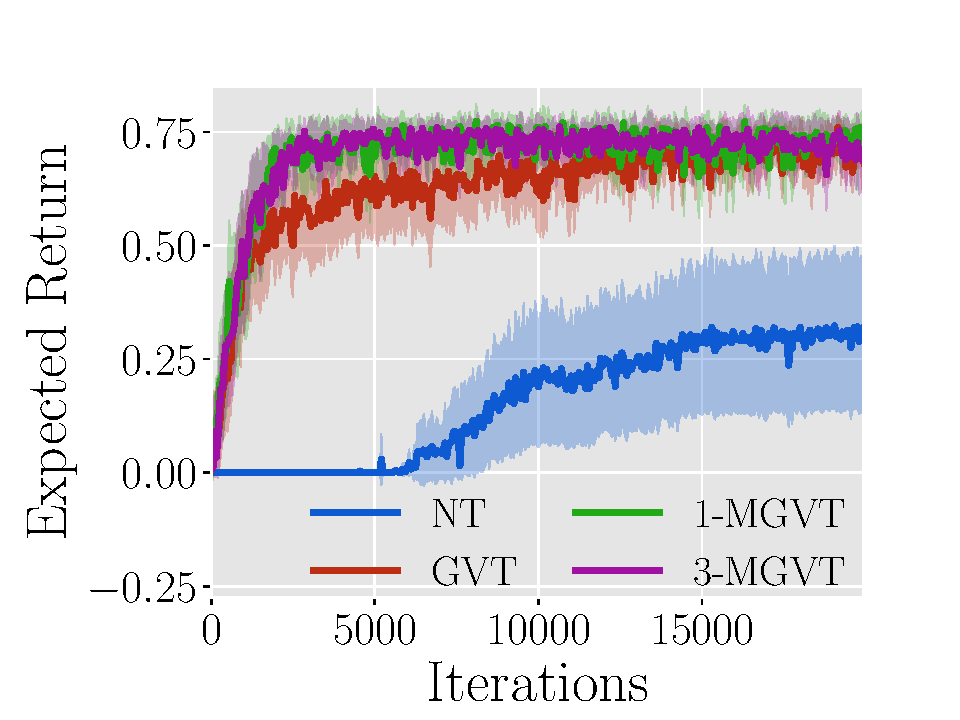
\includegraphics[trim=0.3cm 0cm 1.8cm 1.3cm,clip=true,height=4.5cm]{images/three-room/erew.pdf}
    \caption{}
    \label{fig:3r-erew}
  \end{subfigure}
  \begin{subfigure}[b]{0.45\textwidth}
    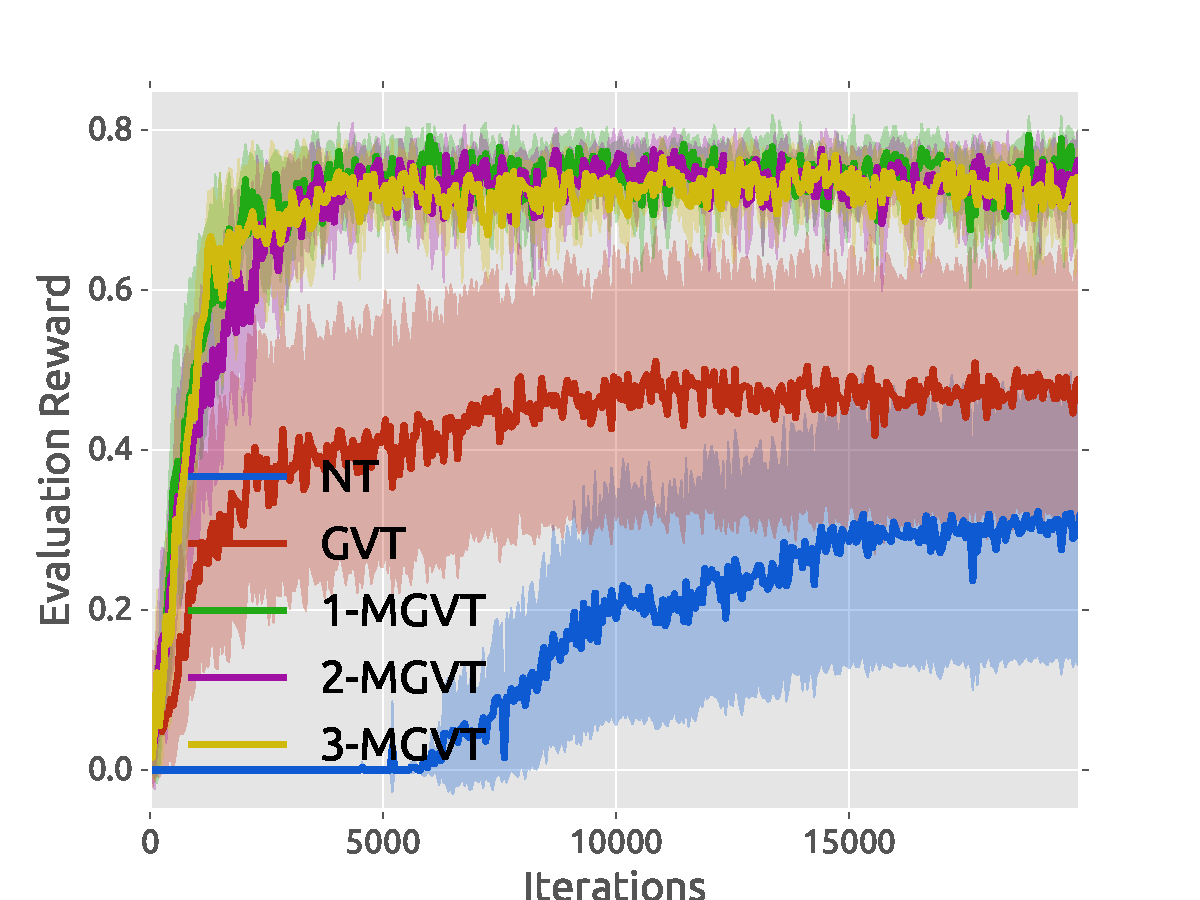
\includegraphics[trim=0.3cm 0cm 1.8cm 1.3cm,clip=true,height=4.5cm]{images/three-room-gen/erew.pdf}
    \caption{}
    \label{fig:3rg-erew}
  \end{subfigure}
  \caption{(a) Rooms Problem: Expected Return w.r.t. Greedy Policy, (b) Rooms Problem: Expected Return w.r.t. Greedy Policy in the generalization experiment}
  \label{fig:rooms-erew}
\end{figure*}

Furthermore, we investigate the exploratory behavior induced by our transfer algorithms and how they differ between each other and in comparison with $\epsilon$-greedy exploration. In Fig. \ref{fig:rooms-expl}, we show the results of running the no transfer (NT) algorithm, GVT and 1-MGVT for $2000$ iterations and we represent as a scatter plot the positions visited by the agent.

\begin{figure*}[b]
  \begin{subfigure}[b]{0.45\textwidth}
    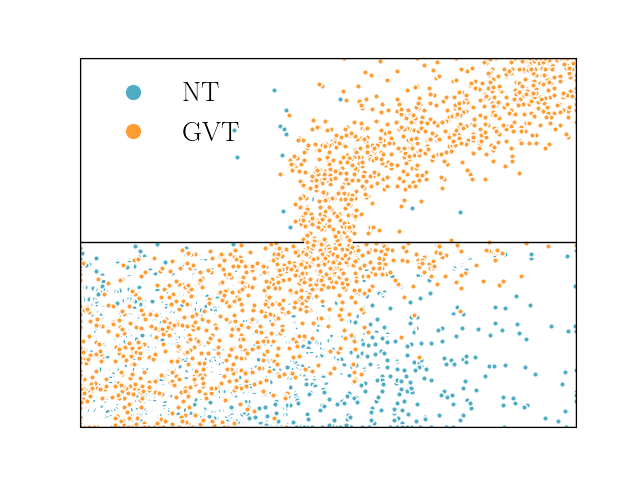
\includegraphics[trim=0.5cm 0.5cm 1.5cm 1.3cm,clip=true,height=4.5cm]{images/three-room-app/nt_vs_gvt.png}
    \caption{}
    \label{fig:nt-vs-gvt}
  \end{subfigure}
  \begin{subfigure}[b]{0.45\textwidth}
    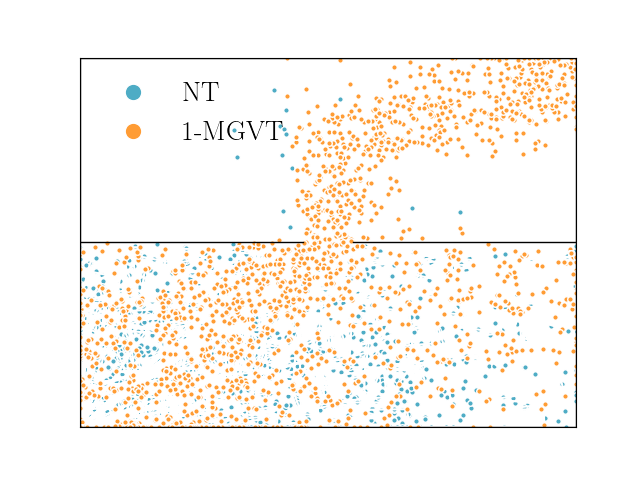
\includegraphics[trim=0.5cm 0.5cm 1.5cm 1.3cm,clip=true,height=4.5cm]{images/three-room-app/nt_vs_mgvt.png}
    \caption{}
    \label{fig:nt-vs-mgvt}
  \end{subfigure}
  \caption{Two-Rooms Problem: (a)  $\epsilon$-greedy vs. GVT, and (b) $\epsilon$-greedy vs. 1-MGVT}
  \label{fig:rooms-expl}
\end{figure*}

Observing Fig. \ref{fig:nt-vs-gvt}, it is possible to understand the difference between the $\epsilon$-greedy exploration and the resulting behavior from GVT. It is noticeable that NT is not capable to lead the agent to the goal within the given iterations as most of the states visited are sparse within the first room, whereas GVT is able to concentrate more of its effort in looking for the door around the middle of the wall. After finding it, within the second room, the positions concentrate in the path leading to the goal given that the need for the exploration is less. This is not surprising as the value function should be equal for all tasks after crossing the door. 

In the other case, we have Fig. \ref{fig:nt-vs-mgvt} that shows a similar situation to that of GVT, but it is quite interesting to notice how sparser the exploration of 1-MGVT is with respect to GVT. Indeed, 1-MGVT is able to actually explore the right part of the first room within these iterations, which might be seen as the result of the prior model being able to capture more information than the Gaussian; hence, the higher speed-up in convergence and robustness to changes in the distribution from which target tasks are drawn. Indeed, as 1-MGVT is able to allow for more flexible exploration, it is capable to discover how to best solve the task much faster than GVT.

In Figure~\ref{fig:sequential} we present the expected return as a function of the number of source tasks used for GVT and MGVT. In particular, we show the resulting curves after $1000$ iterations in Figure~\ref{fig:seq-1000} and after $1950$ iterations in Figure~\ref{fig:seq-1950}. It is interesting to notice the difference on performance between MGVT and GVT whenever there is a small number of source tasks. MGVT clearly provides faster adaptation in the presence of low prior knowledge as it can be discern from the gap seen in nearly a $1000$ iterations between the plots. It is as expected because approximating the prior Gaussian distribution using maximum likelihood estimations with a low number of samples does not provide enough precision. As the number of source tasks increases, as seen more clearly from Figure~\ref{fig:seq-1950}, the performances become closer for this environment.

\begin{figure*}[t]
  \begin{subfigure}[b]{0.45\textwidth}
    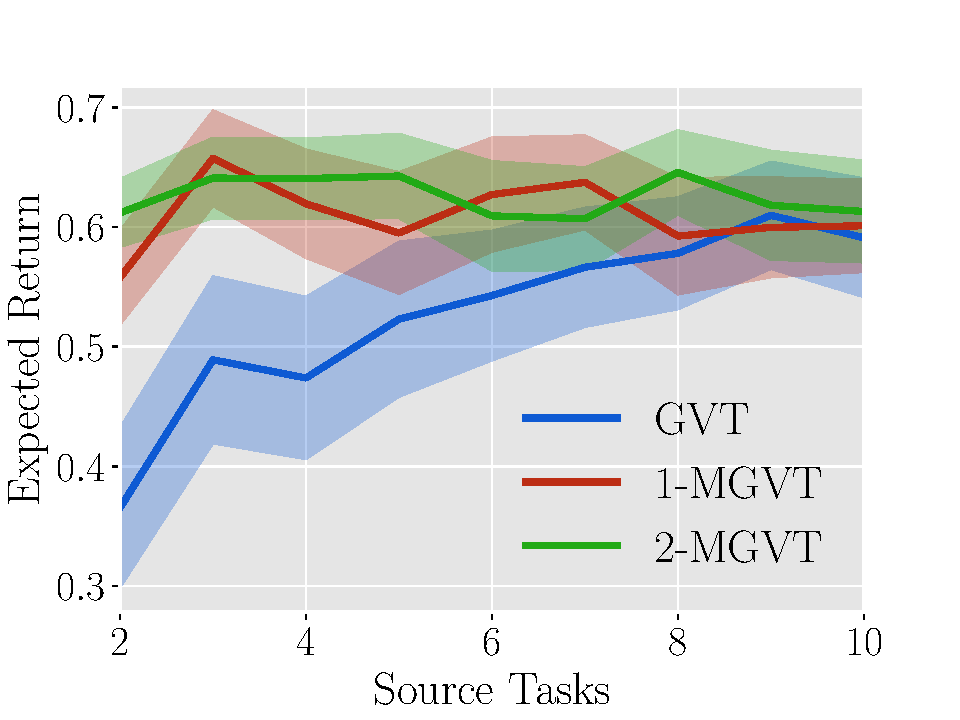
\includegraphics[trim=0.0cm 0cm 1.2cm 1.3cm,clip=true,height=4.5cm]{images/sequential/lrew_1000.pdf}
    \caption{}
    \label{fig:seq-1000}
  \end{subfigure}
  \begin{subfigure}[b]{0.45\textwidth}
    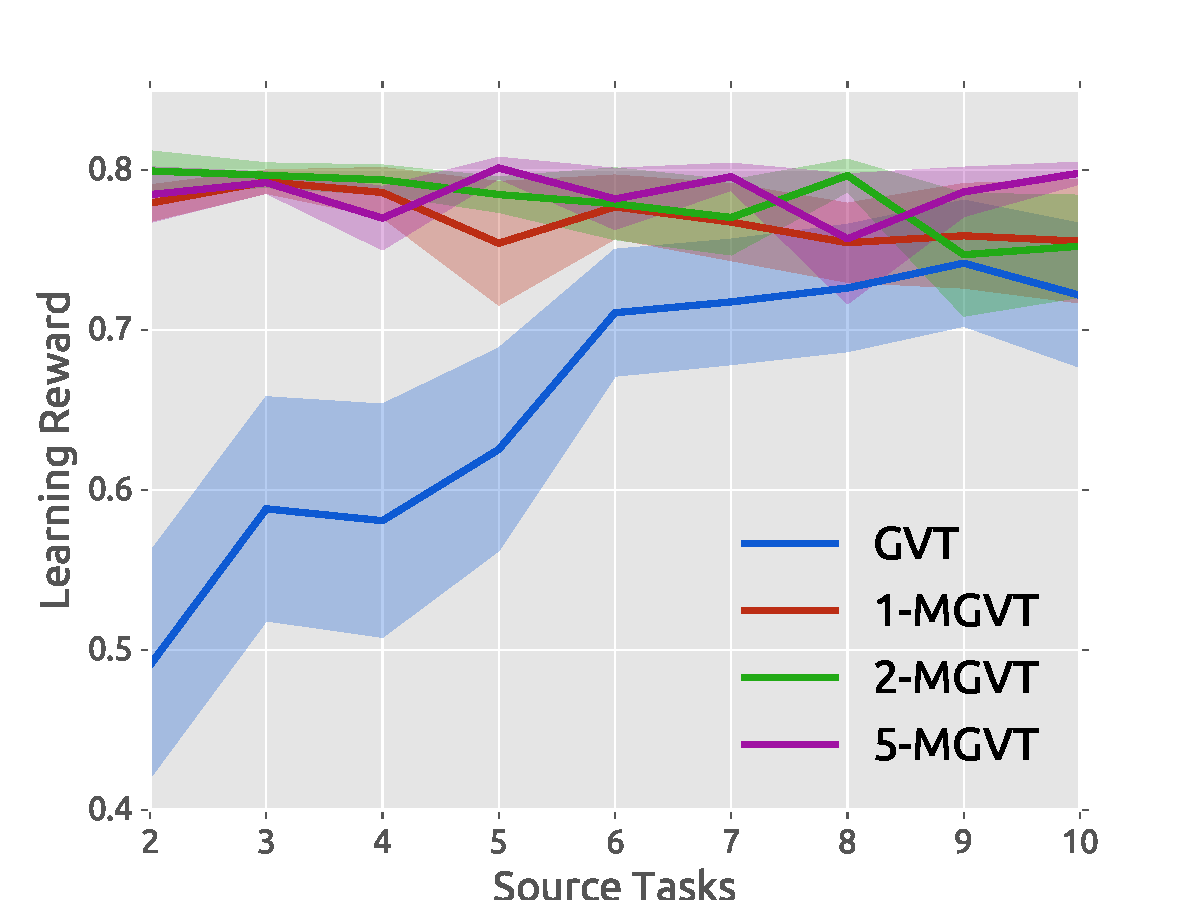
\includegraphics[trim=0.0cm 0cm 1.2cm 1.3cm,clip=true,height=4.5cm]{images/sequential/lrew_1950.pdf}
    \caption{}
    \label{fig:seq-1950}
  \end{subfigure}
  \caption{Expected return w.r.t. to the number of source tasks (a) $1000$ iterations, (b) $1950$ iterations}
  \label{fig:sequential}
\end{figure*}

Finally, we analyze the transfer performance as a function of how likely the target task is according to the prior. We consider a two-room version of the environment of Figure~\ref{fig:main}. Unlike before, we generate tasks by sampling the door position from a Gaussian with mean $5$ and standard deviation $1.8$, so that tasks with the door near the sides are very unlikely. Figure~\ref{fig:likelihood} shows the performance reached by GVT and 1-MGVT at fixed iterations as a function of how likely the target task is according to such distribution. As expected, GVT achieves poor performance on very unlikely tasks, even after many iterations. In fact, estimating a single Gaussian distribution definitely entails some information loss, especially about the unlikely tasks. On the other hand, MGVT keeps such information and, consequently, performs much better. Perhaps not surprisingly, MGVT reaches the optimal performance in $4k$ iterations no matter what task is being solved.

\begin{figure*}[t]
\centering
    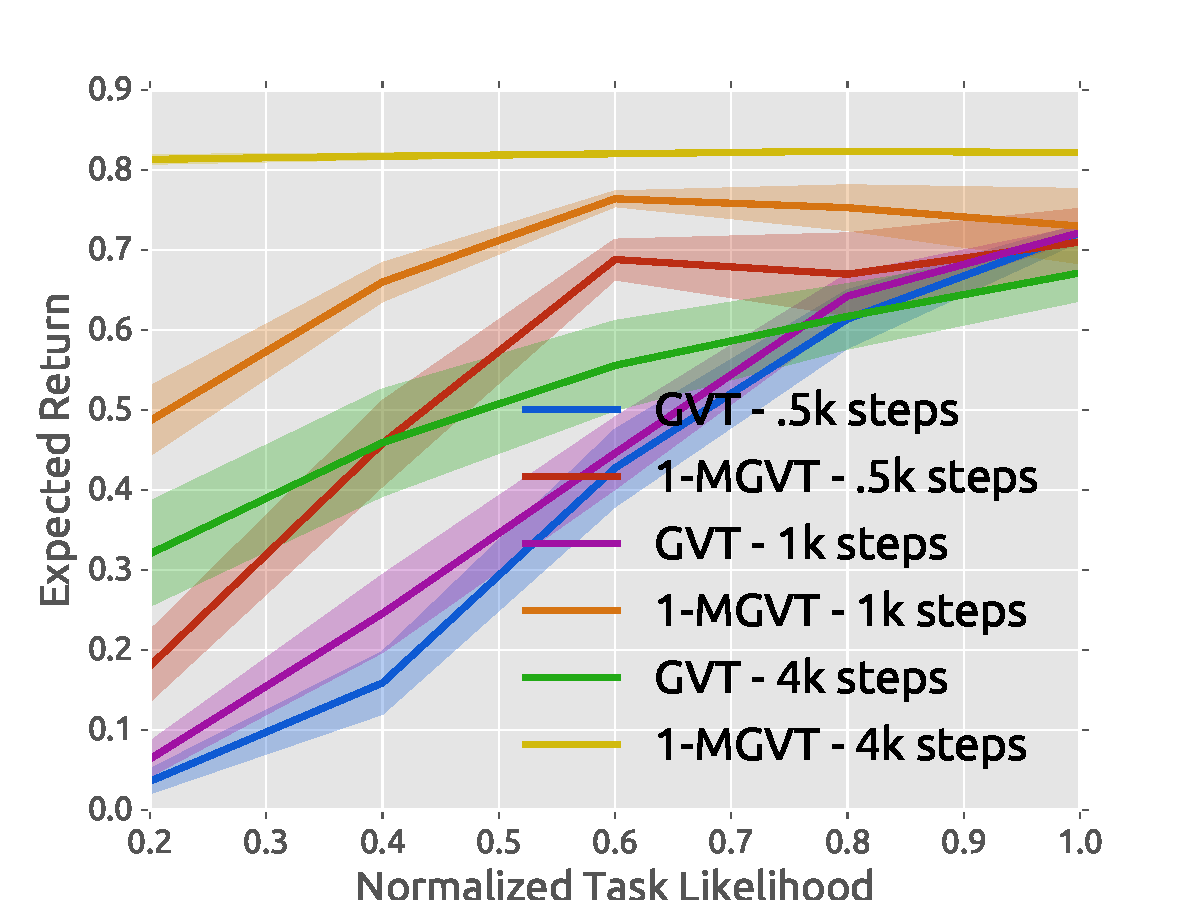
\includegraphics[trim=0.0cm 0cm 1.2cm 1.3cm,clip=true,height=4.5cm]{images/likelihood/lrew.pdf}
    \caption{Expected return as a function of the task likelihood.}
  \label{fig:likelihood}
\end{figure*}


\subsection{Classic Control}\label{app:c2}

\subsubsection{Cartpole}

For this environment we generate tasks by uniformly sampling the cart mass in the range $\left[0.5,1.5\right]$, the pole mass in $\left[0.1,0.3\right]$ and the pole length in $\left[0.2,1.0\right]$. 

During the training of the source tasks, we use a \textit{batch size} of $150$ and a \textit{buffer size} of $50000$. Specifically, for DDQN we use a \textit{target update frequency} of $500$,\textit{exploration fraction} of $0.35$ and a learning rate $\alpha=0.001$. We use a Multilayer Perceptron (MLP) with ReLU as activation function and a single hidden layer of $32$ neurons.

For the transfer experiments, we set the \textit{batch size} to $500$, the number of \textit{weights} sampled to approximate the expected TD error to $5$, $\lambda=0.001$ and $\psi=0.5\ $. We use $\alpha_{\mu}=0.001$ as the learning rate for the mean of the Gaussian posterior. For its the Cholesky factor L we use $\alpha_L=0.0001$ and set the limit that the minimum eigenvalue may reach to $\sigma_{min}^2=0.0001\ $. Additionally, for MGVT we set the variance of the prior components $\sigma_p^2=10^{-5}$ and leave the learning rates of the posterior components' means and Cholesky factor the same as GVT.

In Figure~\ref{fig:cp-erew}, we show the greedy performance of DDQN, GVT, 1-MGVT and 3-MGVT, as in the previous section. Once again, we can see how the transfer methods provide a significant jump-start w.r.t. the DDQN evaluation.

\begin{figure*}[t]
  \begin{subfigure}[b]{0.45\textwidth}
    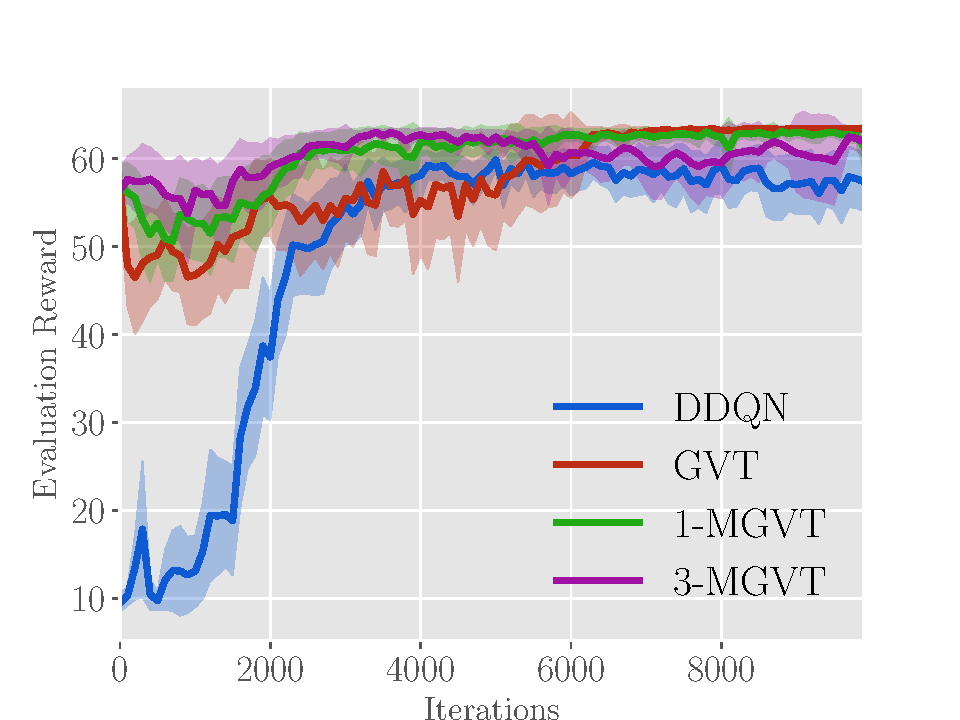
\includegraphics[trim=0.0cm 0cm 1.8cm 1.3cm,clip=true,height=4.5cm]{images/cartpole/erew.pdf}
    \caption{}
    \label{fig:cp-erew}
  \end{subfigure}
  \begin{subfigure}[b]{0.45\textwidth}
    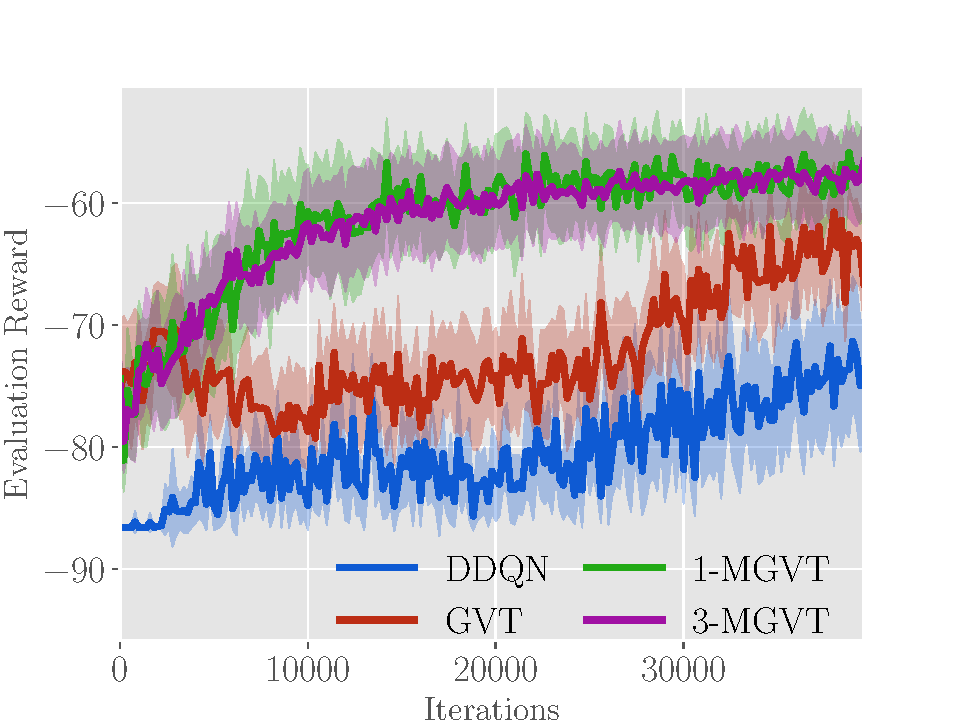
\includegraphics[trim=0.0cm 0cm 1.8cm 1.3cm,clip=true,height=4.5cm]{images/mountaincar/erew.pdf}
    \caption{}
    \label{fig:mc-erew}
  \end{subfigure}
  \caption{(a) Cartpole: Expected Return w.r.t. Greedy Policy, (b) Mountain Car: Expected Return w.r.t. Greedy Policy}
  \label{fig:ccerew}
\end{figure*}

\subsubsection{Mountain Car}

We generate tasks sampling uniformly the base speed of the actions in the range $\left[0.001, 0.0015\right]$. 

For the sources, we train the tasks using DDQN with a \textit{target update frequency} of $500$, a \textit{batch size} of $32$, a  \textit{buffer size} of $50000$ and learning rate $\alpha=0.001$. Moreover, we set the \textit{exploration fraction} to $0.15$. We use an MLP with single hidden layer of $64$ neurons with ReLU activation function. 

For the transfer experiments, we set the \textit{batch size} to $500$, and use $10$ \textit{weights} to approximate the expected TD error, $\lambda=10^{-5}$ and $\psi=0.5$. For the learning rates, we use $\alpha_{\mu}=0.001$ for the means of the Gaussians. In the case of the Cholesky factors L, we use $\alpha_L=0.0001$ and allow the eigenvalues to reach a minimum value of $\sigma_{min}^2=0.0001$. In the case of MGVT, additionally, we set the prior covariance to be $\sigma_p^2=10^{-5}$.

In Figure~\ref{fig:mc-erew}, we show the greedy performance obtained during the executions, as in the previous sections. In this plot, we can observe directly how fast is MGVT able to converge its mean to the actual optimal performance and that even if GVT struggles to learn in comparison with MGVT, still provides a clear advantage w.r.t. DDQN. Also, it is worth noting that the variances seen are result that different speeds of the car result in different time to reach the goal and, thus, different optimal performances.

Clearly, this variation in the values among tasks allows MGVT to excel w.r.t. to the other methods. The richer prior of MGVT allows to exploit efficiently the previous knowledge on the possible values attainable from the tasks and, therefore, quickly resolve how to best optimize for the target. This fact is a clear contrast with GVT as the search is more likely constrained to the mean values and moving away from that is, in fact, slower.

\subsection{Maze Navigation}\label{app:c3}

The mazes adopted in the experiments of Section \ref{sec:exp} are shown in Fig.~\ref{fig:mazes}. Our $20$ mazes have varying degree of difficulty and are designed to hold few similarities that would be useful for transferring. Moreover, we ensure $4$ groups of mazes that are characterized by their goal position. 

For the experiments we use as an approximator an MLP with two hidden layers of $32$ neurons with ReLU activation functions. For training the sources we use a DDQN with a \textit{batch size} of $70$, a \textit{buffer size} of $10000$ and a \textit{target update frequency} of $100$, setting the \textit{exploration fraction} to $0.1$ and learning rate to $\alpha=0.001$.

In the transfer experiments we use $\psi=0.5$, a \textit{batch size} of $50$, a \textit{buffer size} of $50000$ and use $10$ sampled \textit{weights} from the posterior to approximate the TD error. Moreover, we use $\lambda=10^{-6}$. For GVT, in particular, we use $\alpha_{\mu}=0.001$, $\alpha_{L}=10^{-7}$, and set the minimum value reachable by its eigenvalues to be $\sigma_{min}=0.0001$. In the case of MGVT, we set $\alpha_{\mu}=0.001$ and $\alpha_{L}=10^{-6}$. Finally, we use $\sigma_p^2=10^{-5}$ as the prior bandwidth.


\begin{figure*}[t]
\centering
\begin{subfigure}[t]{0.18\textwidth}
    
\includegraphics[width=\textwidth]{images/maze/maze0.pdf}
    \caption{} \label{fig:maze0}
  \end{subfigure}
  \begin{subfigure}[t]{0.18\textwidth}
    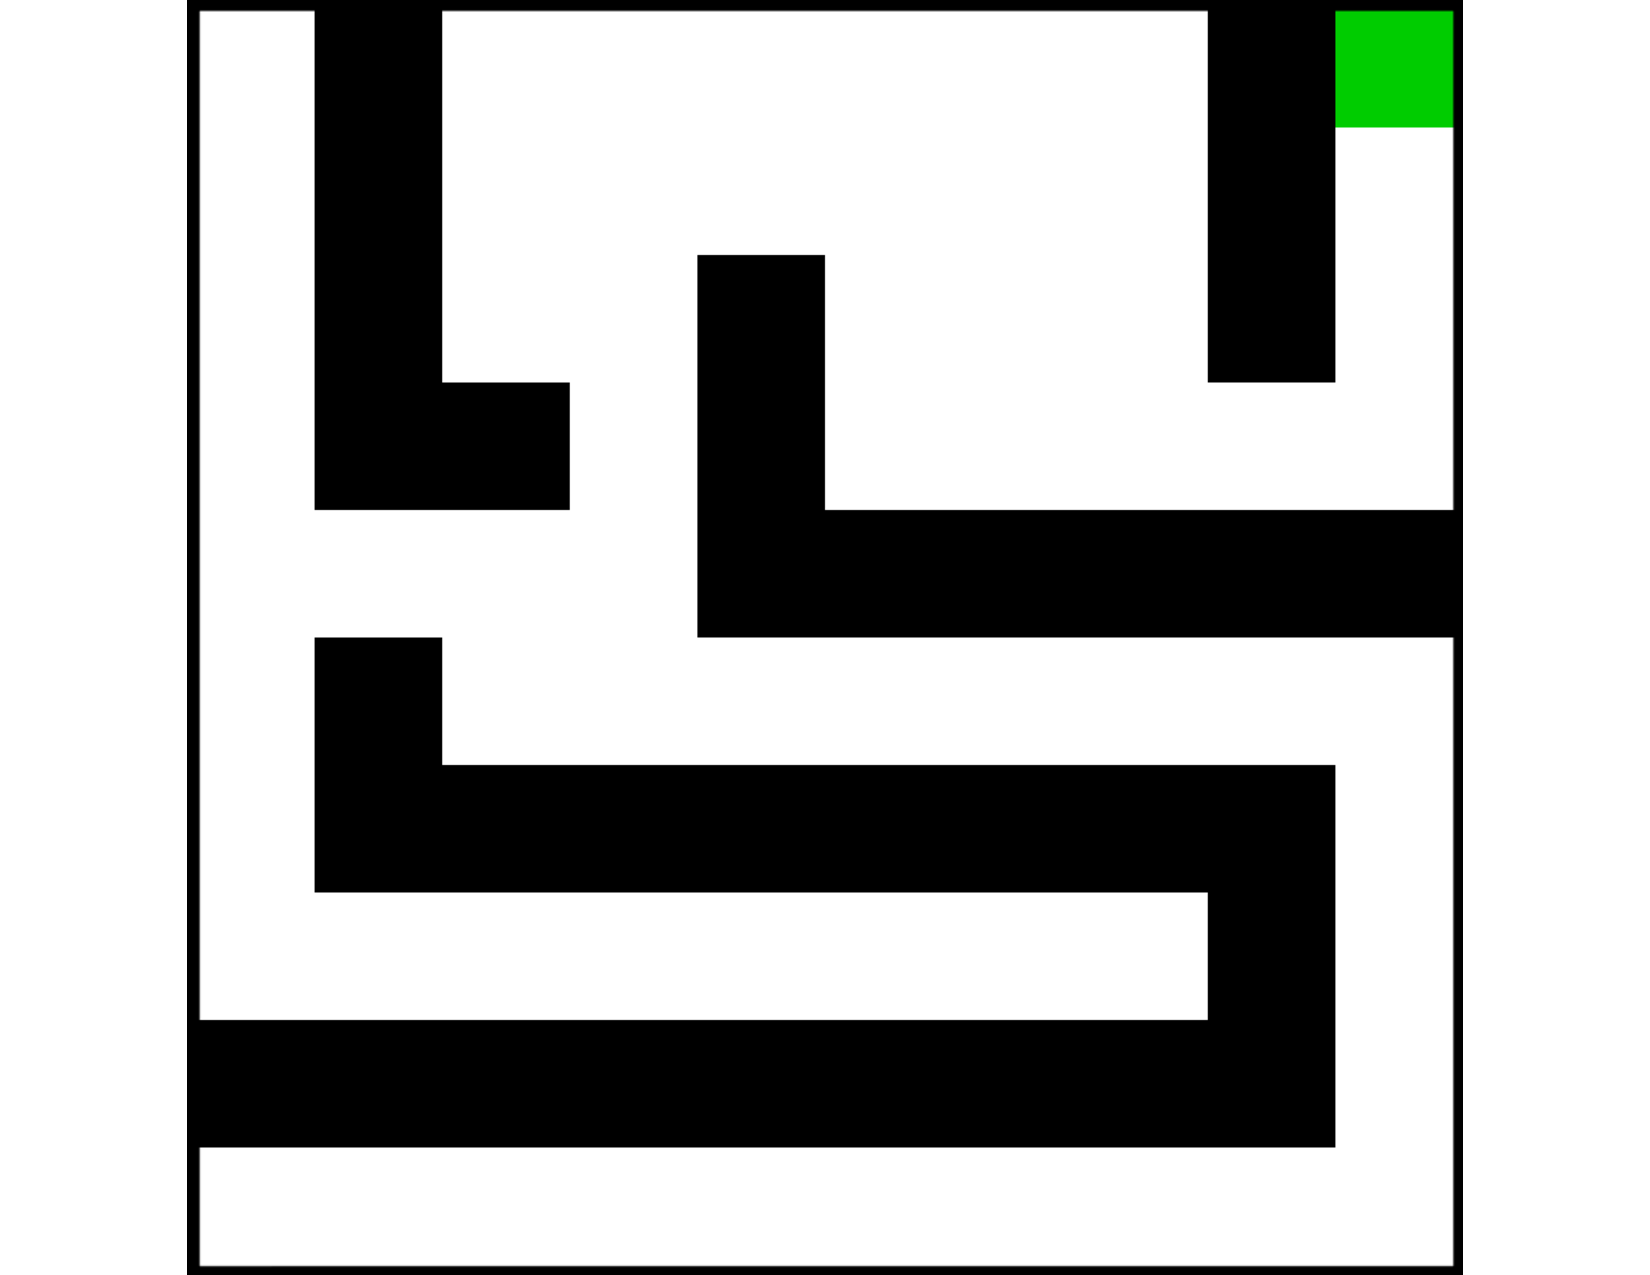
\includegraphics[width=\textwidth]{images/maze/maze1.pdf}
    \caption{}
  \end{subfigure}
  \begin{subfigure}[t]{0.18\textwidth}
    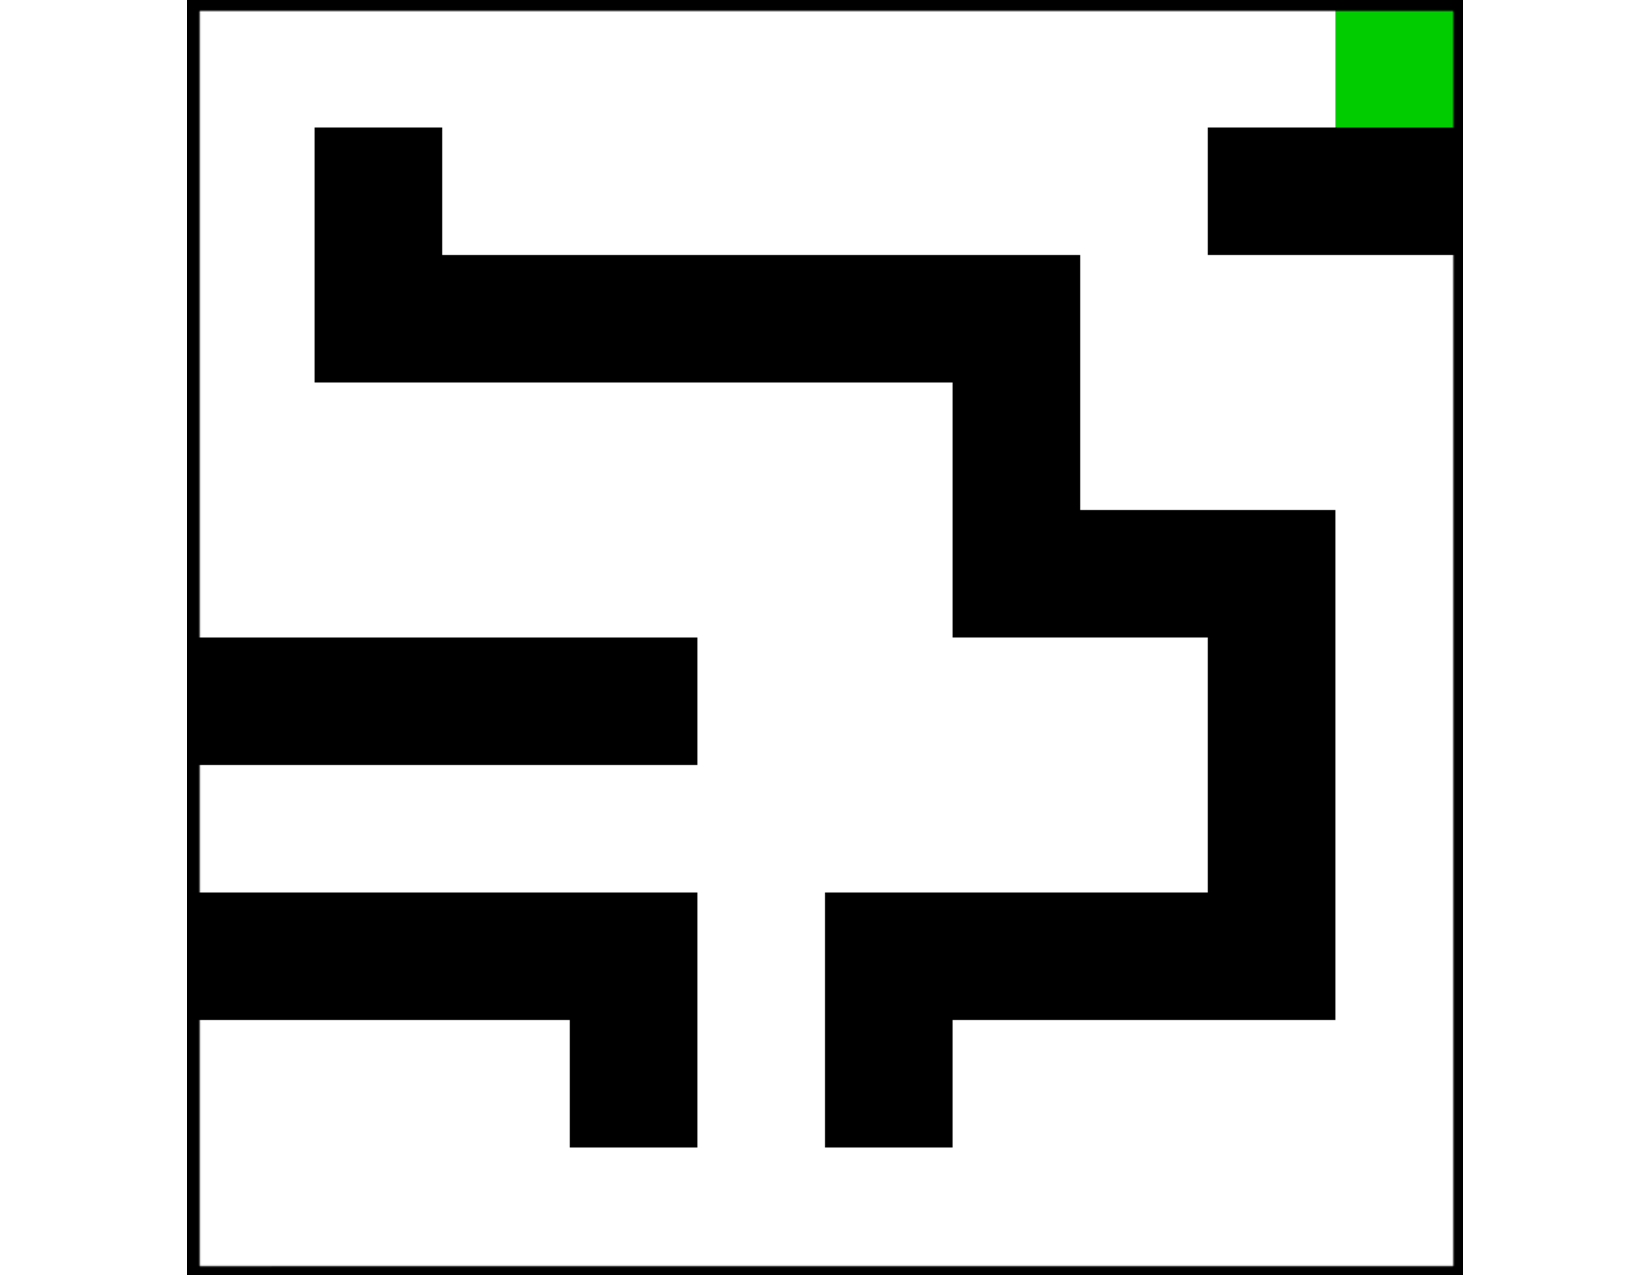
\includegraphics[width=\textwidth]{images/maze/maze2.pdf}
    \caption{}
  \end{subfigure}
  \begin{subfigure}[t]{0.18\textwidth}
    
\includegraphics[width=\textwidth]{images/maze/maze3.pdf}
    \caption{}
  \end{subfigure}
  \begin{subfigure}[t]{0.18\textwidth}
    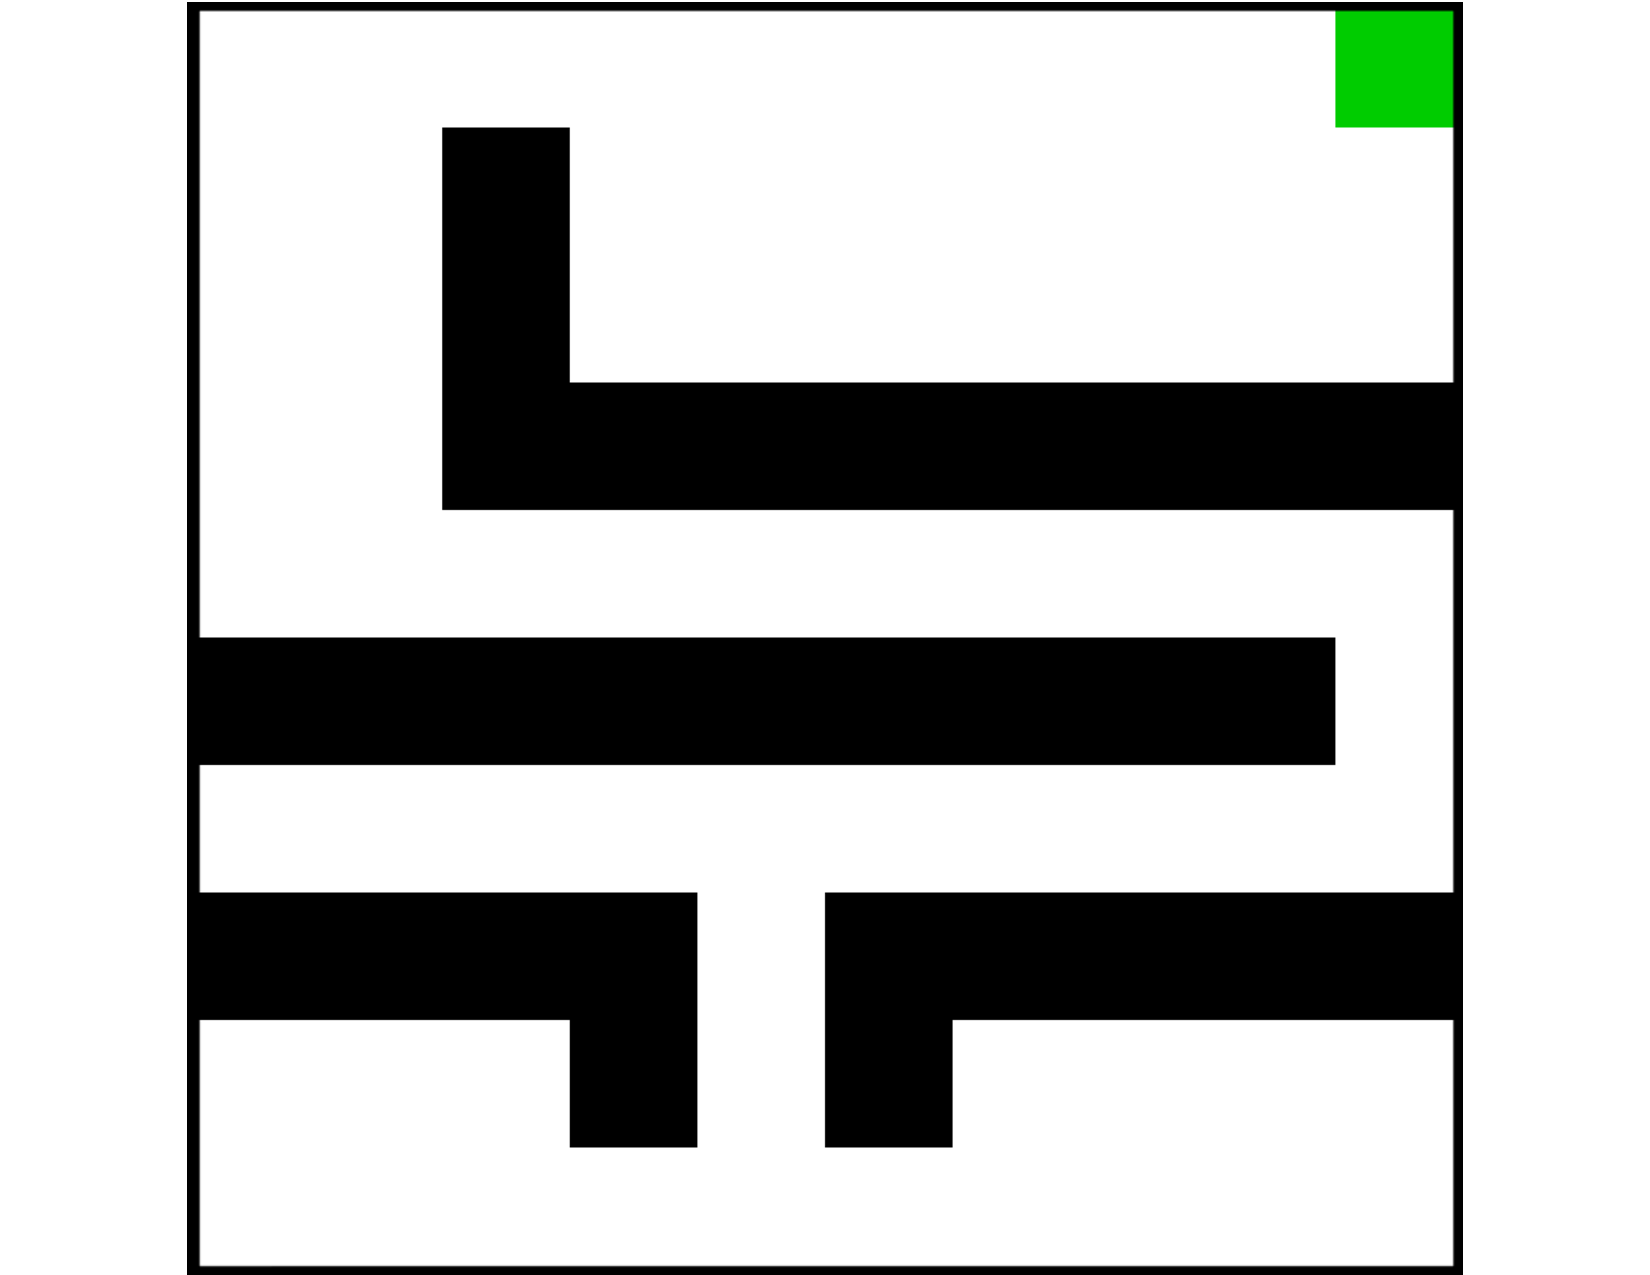
\includegraphics[width=\textwidth]{images/maze/maze4.pdf}
    \caption{}
  \end{subfigure}
  
  \begin{subfigure}[t]{0.18\textwidth}
    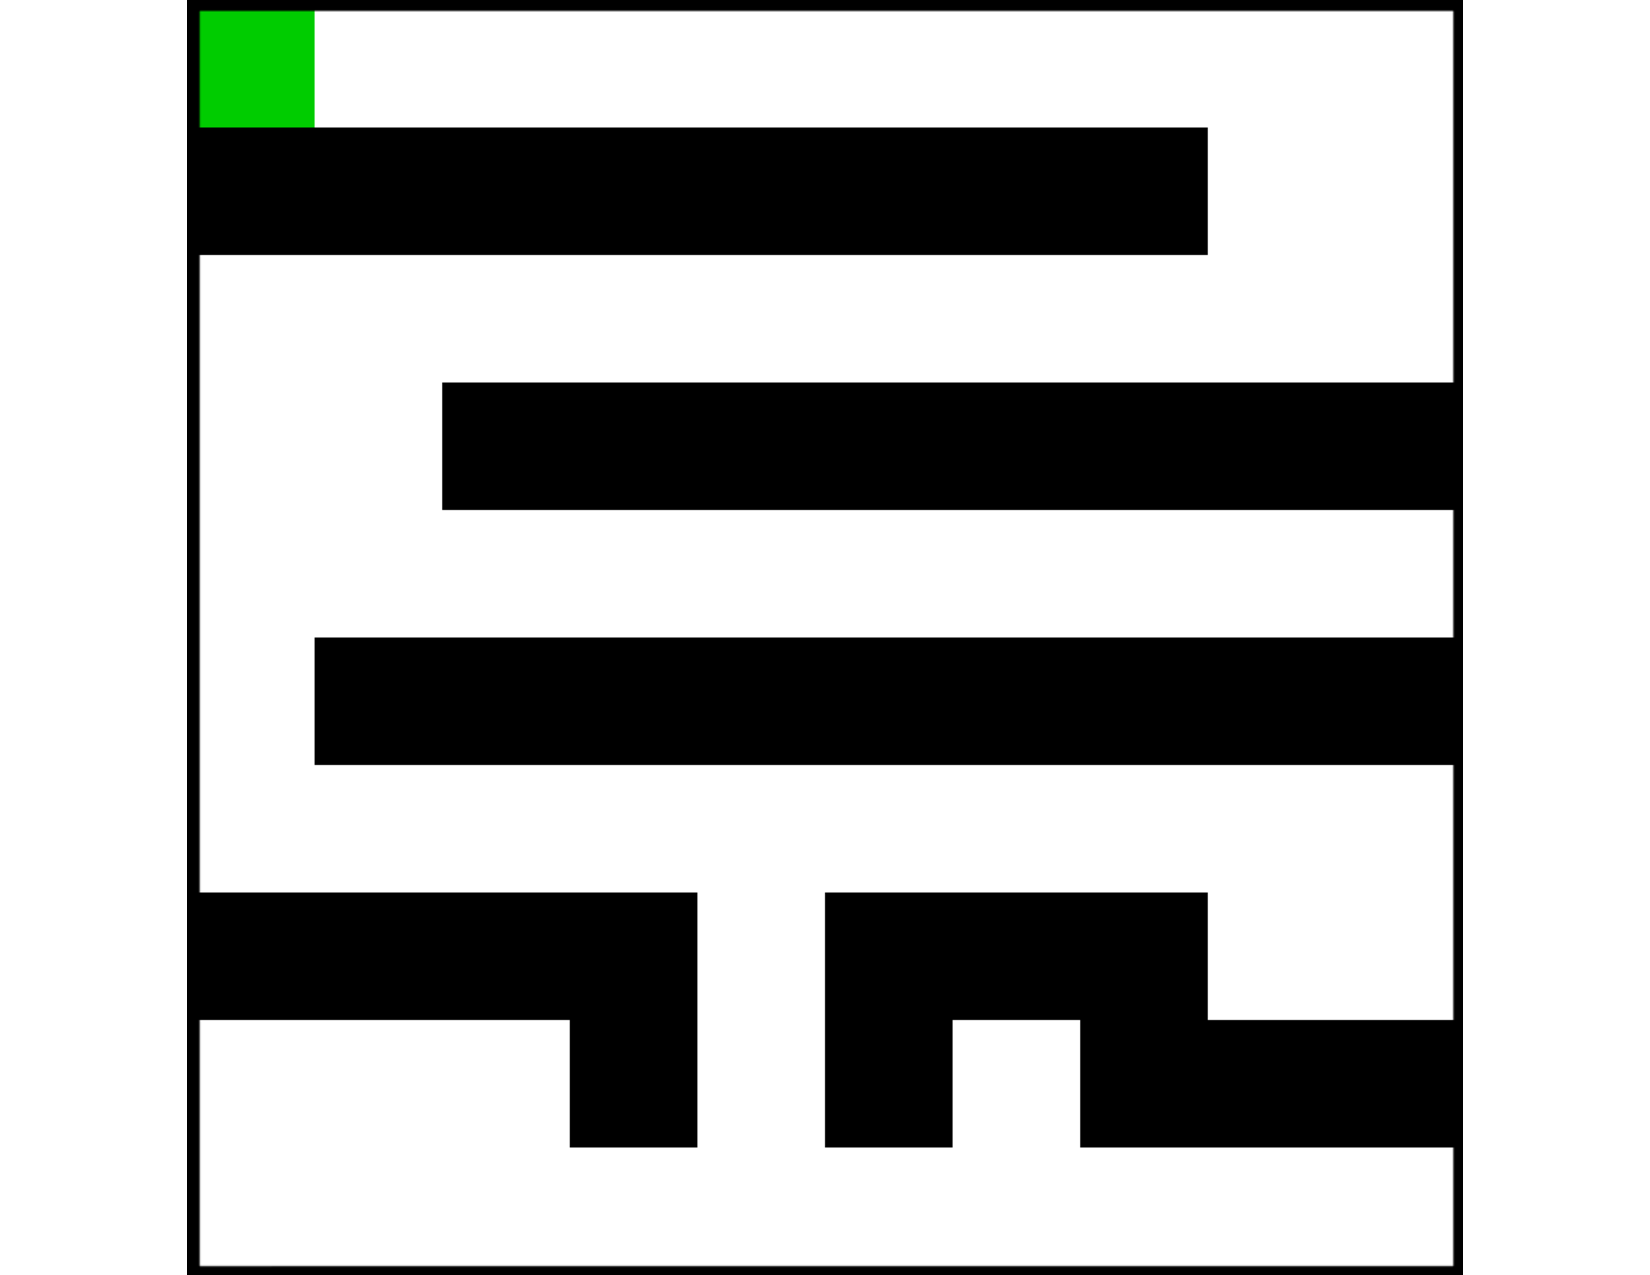
\includegraphics[width=\textwidth]{images/maze/maze5.pdf}
    \caption{}
  \end{subfigure}
  \begin{subfigure}[t]{0.18\textwidth}
    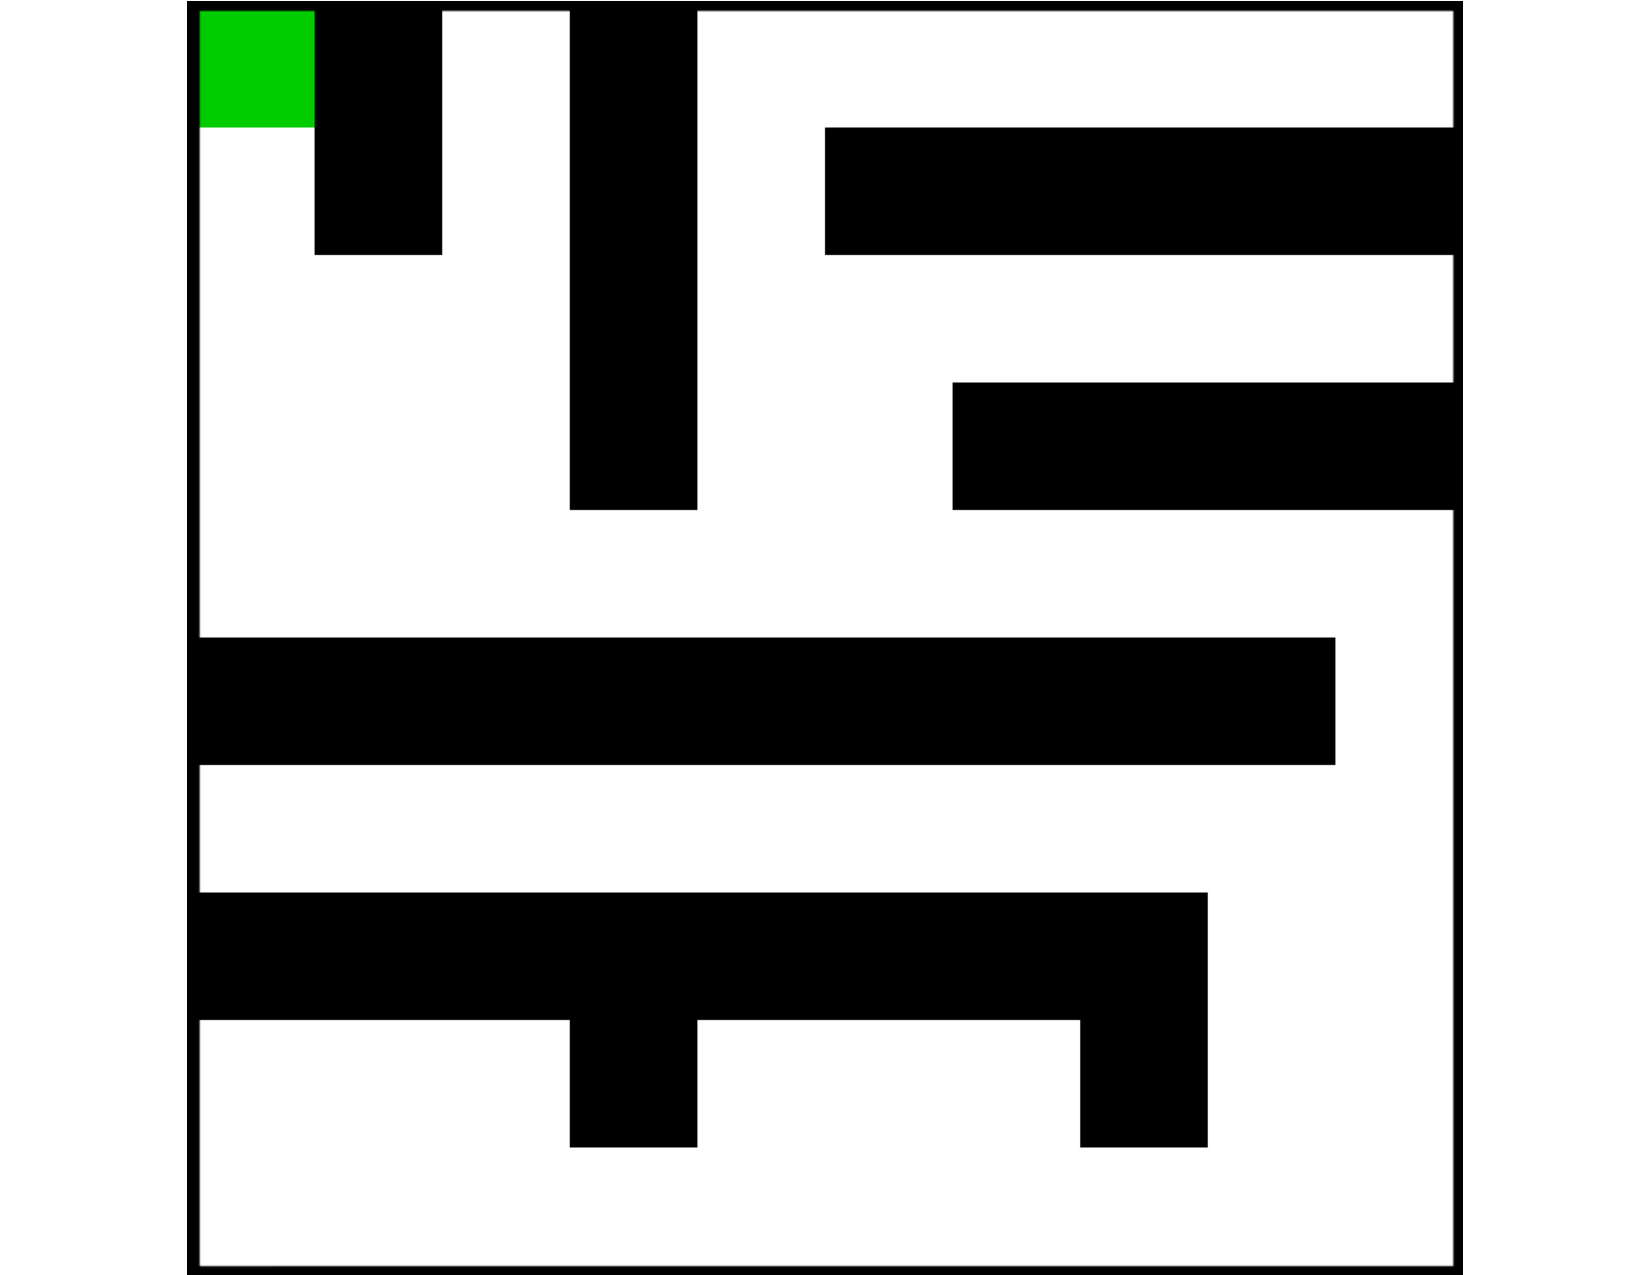
\includegraphics[width=\textwidth]{images/maze/maze6.pdf}
    \caption{}\label{fig:maze6}
  \end{subfigure}
  \begin{subfigure}[t]{0.18\textwidth}
    
\includegraphics[width=\textwidth]{images/maze/maze7.pdf}
    \caption{}
  \end{subfigure}
  \begin{subfigure}[t]{0.18\textwidth}
    
\includegraphics[width=\textwidth]{images/maze/maze8.pdf}
    \caption{}\label{fig:maze8}
  \end{subfigure}
  \begin{subfigure}[t]{0.18\textwidth}
    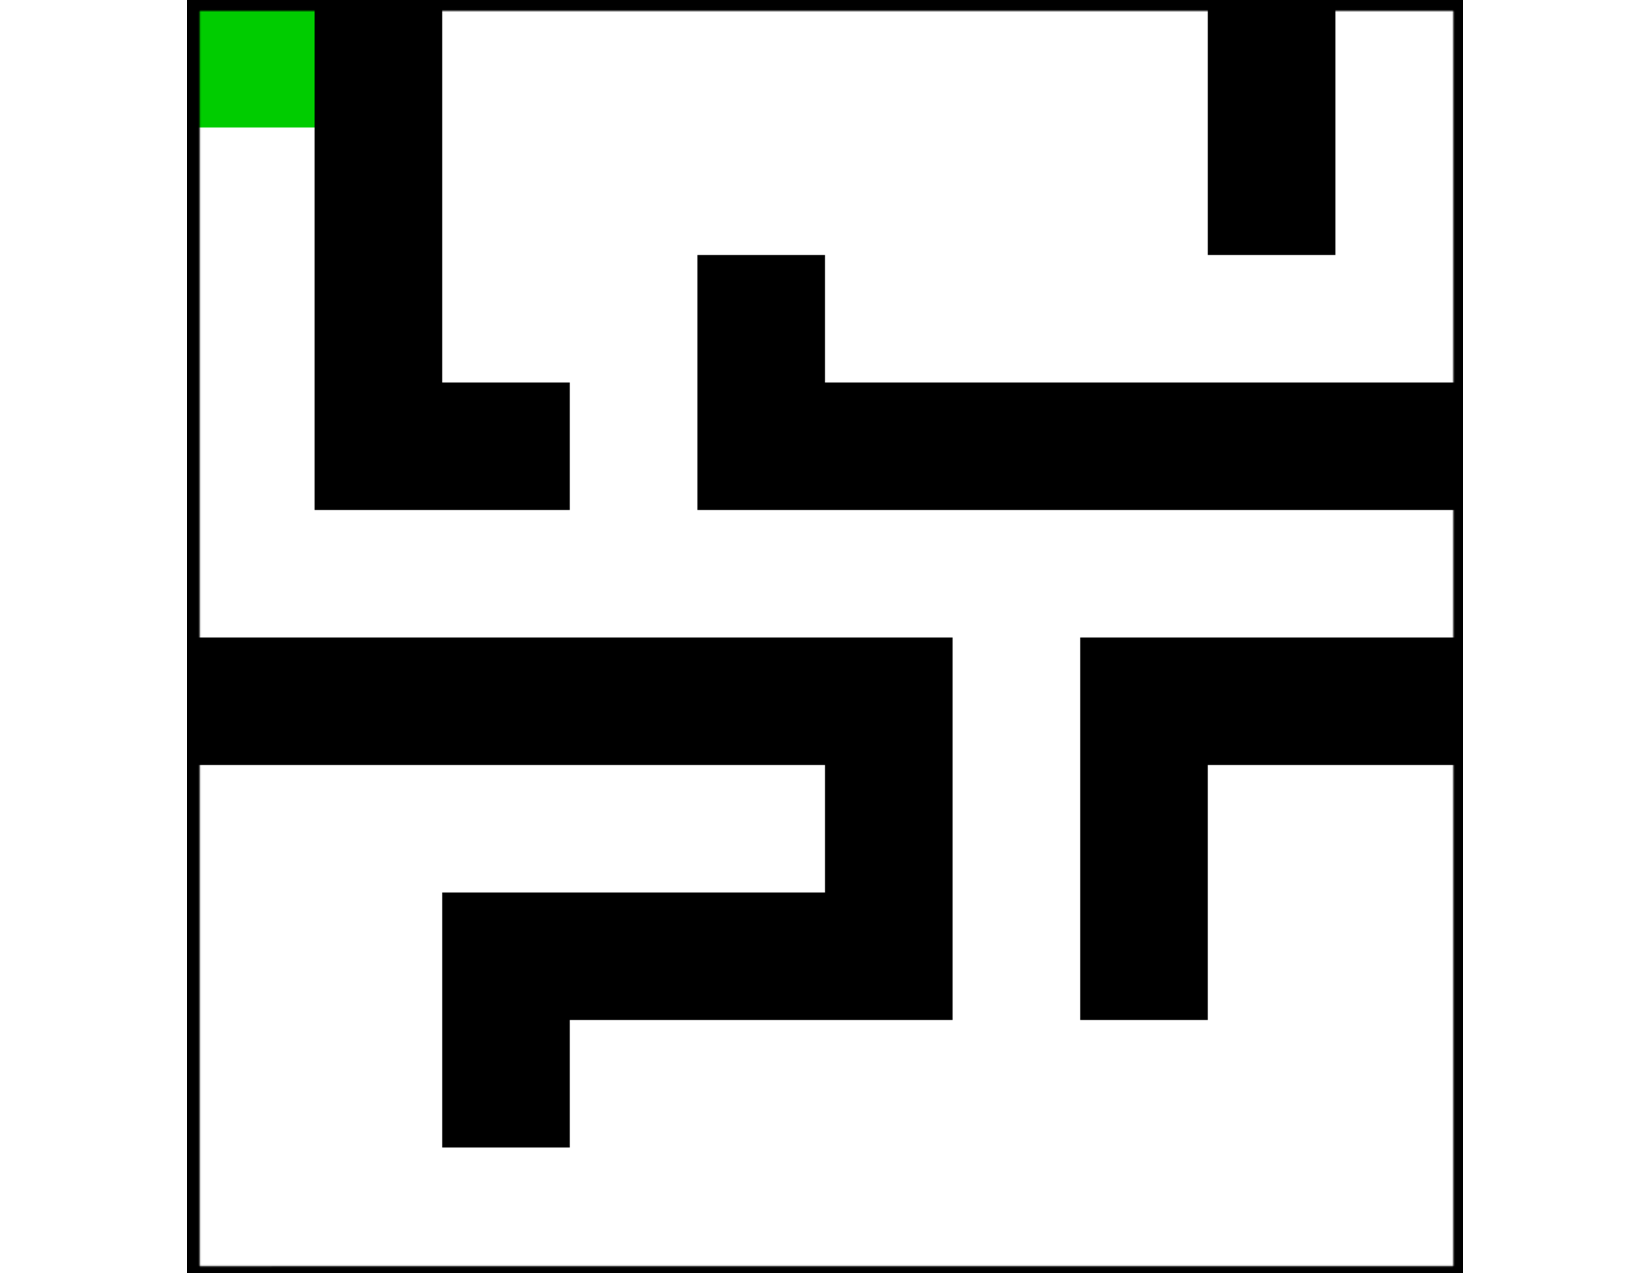
\includegraphics[width=\textwidth]{images/maze/maze9.pdf}
    \caption{}
  \end{subfigure}
  
  \begin{subfigure}[t]{0.18\textwidth}
    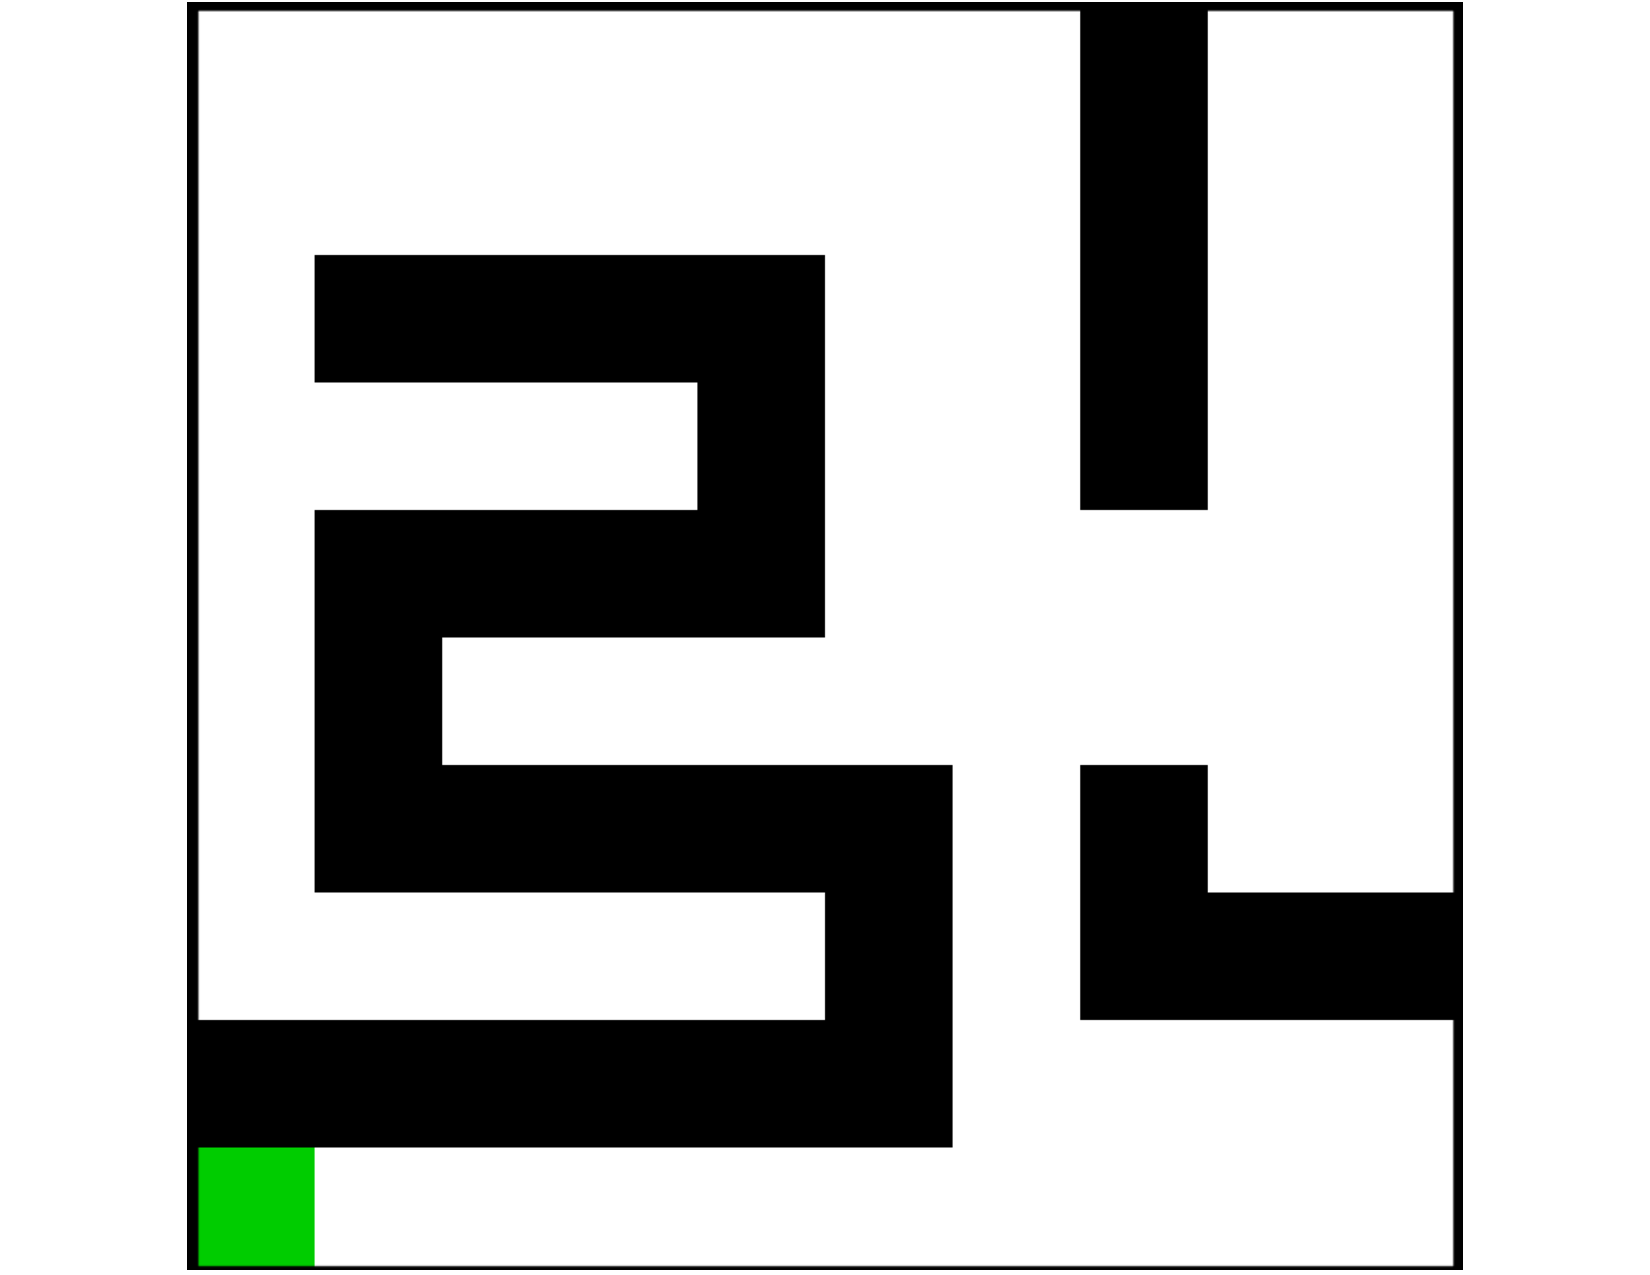
\includegraphics[width=\textwidth]{images/maze/maze10.pdf}
    \caption{}
  \end{subfigure}
  \begin{subfigure}[t]{0.18\textwidth}
    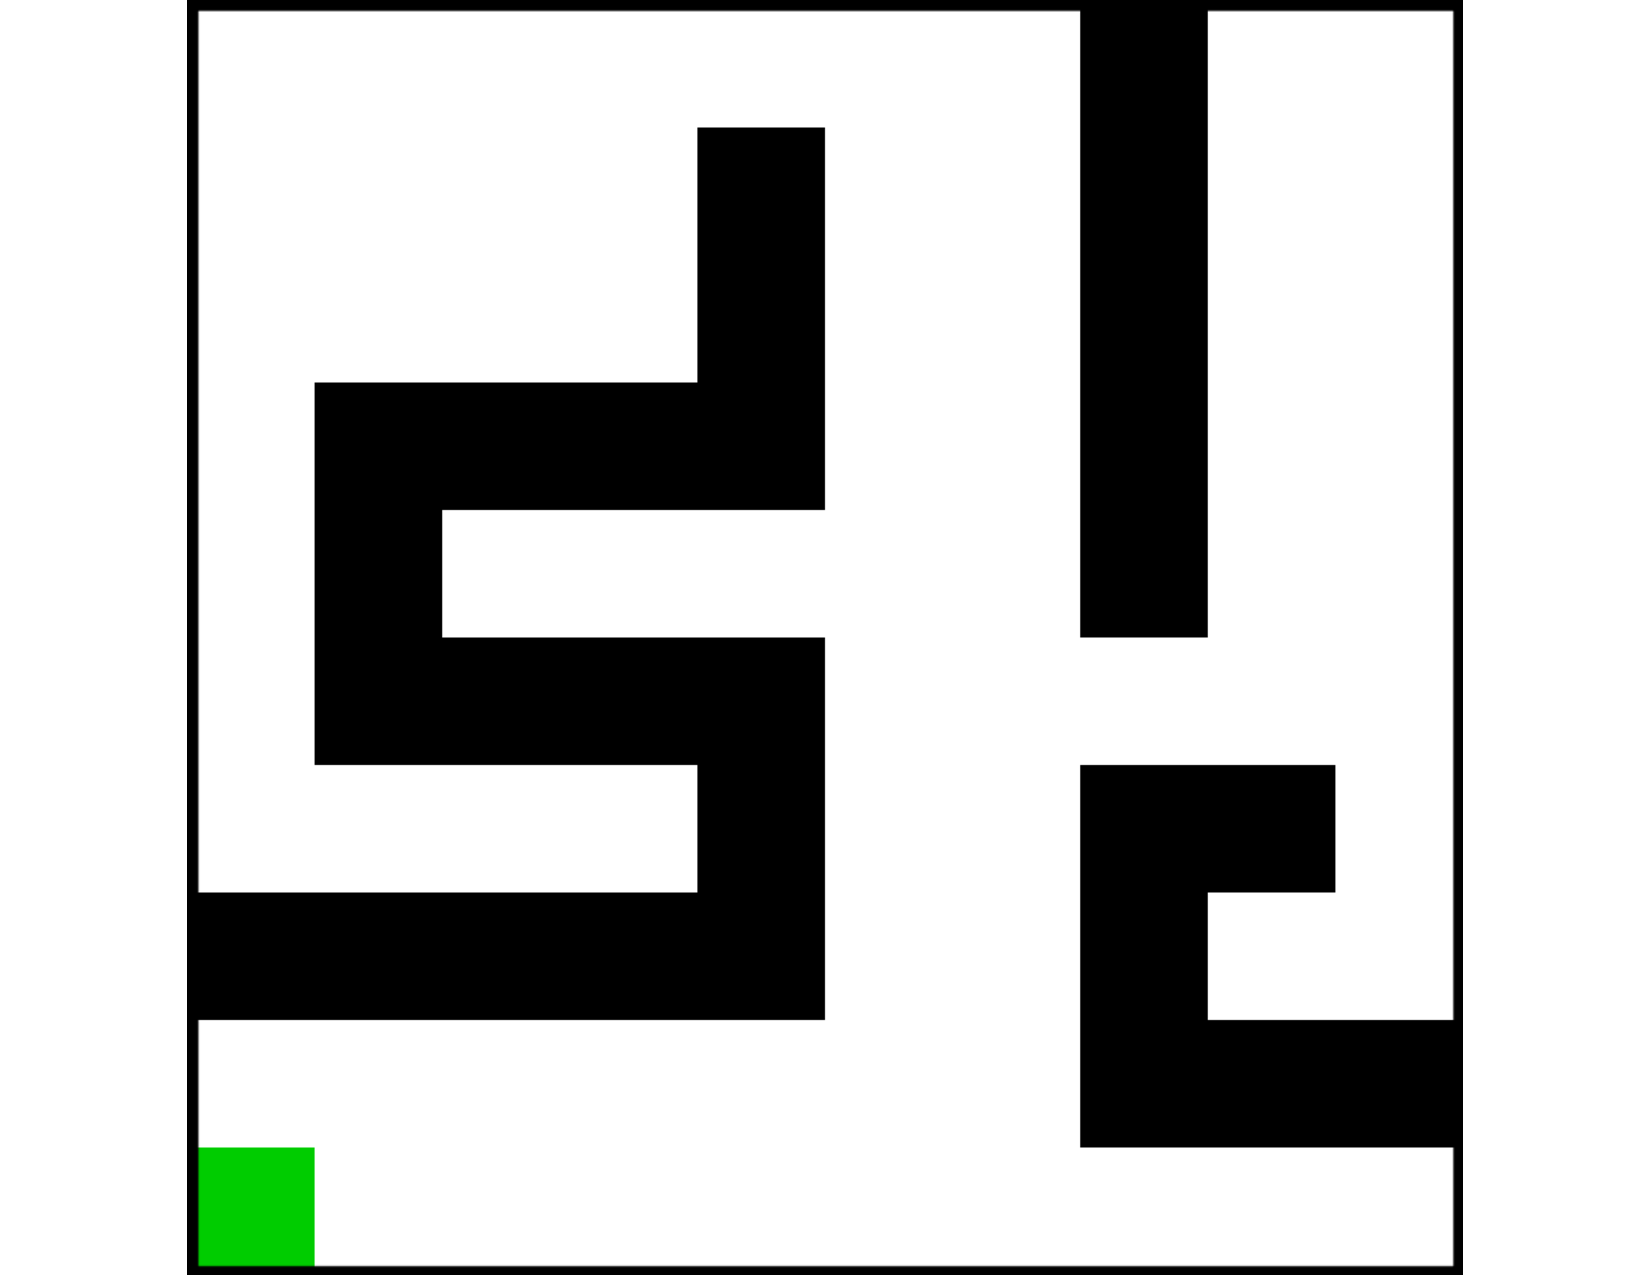
\includegraphics[width=\textwidth]{images/maze/maze11.pdf}
    \caption{}
  \end{subfigure}
  \begin{subfigure}[t]{0.18\textwidth}
    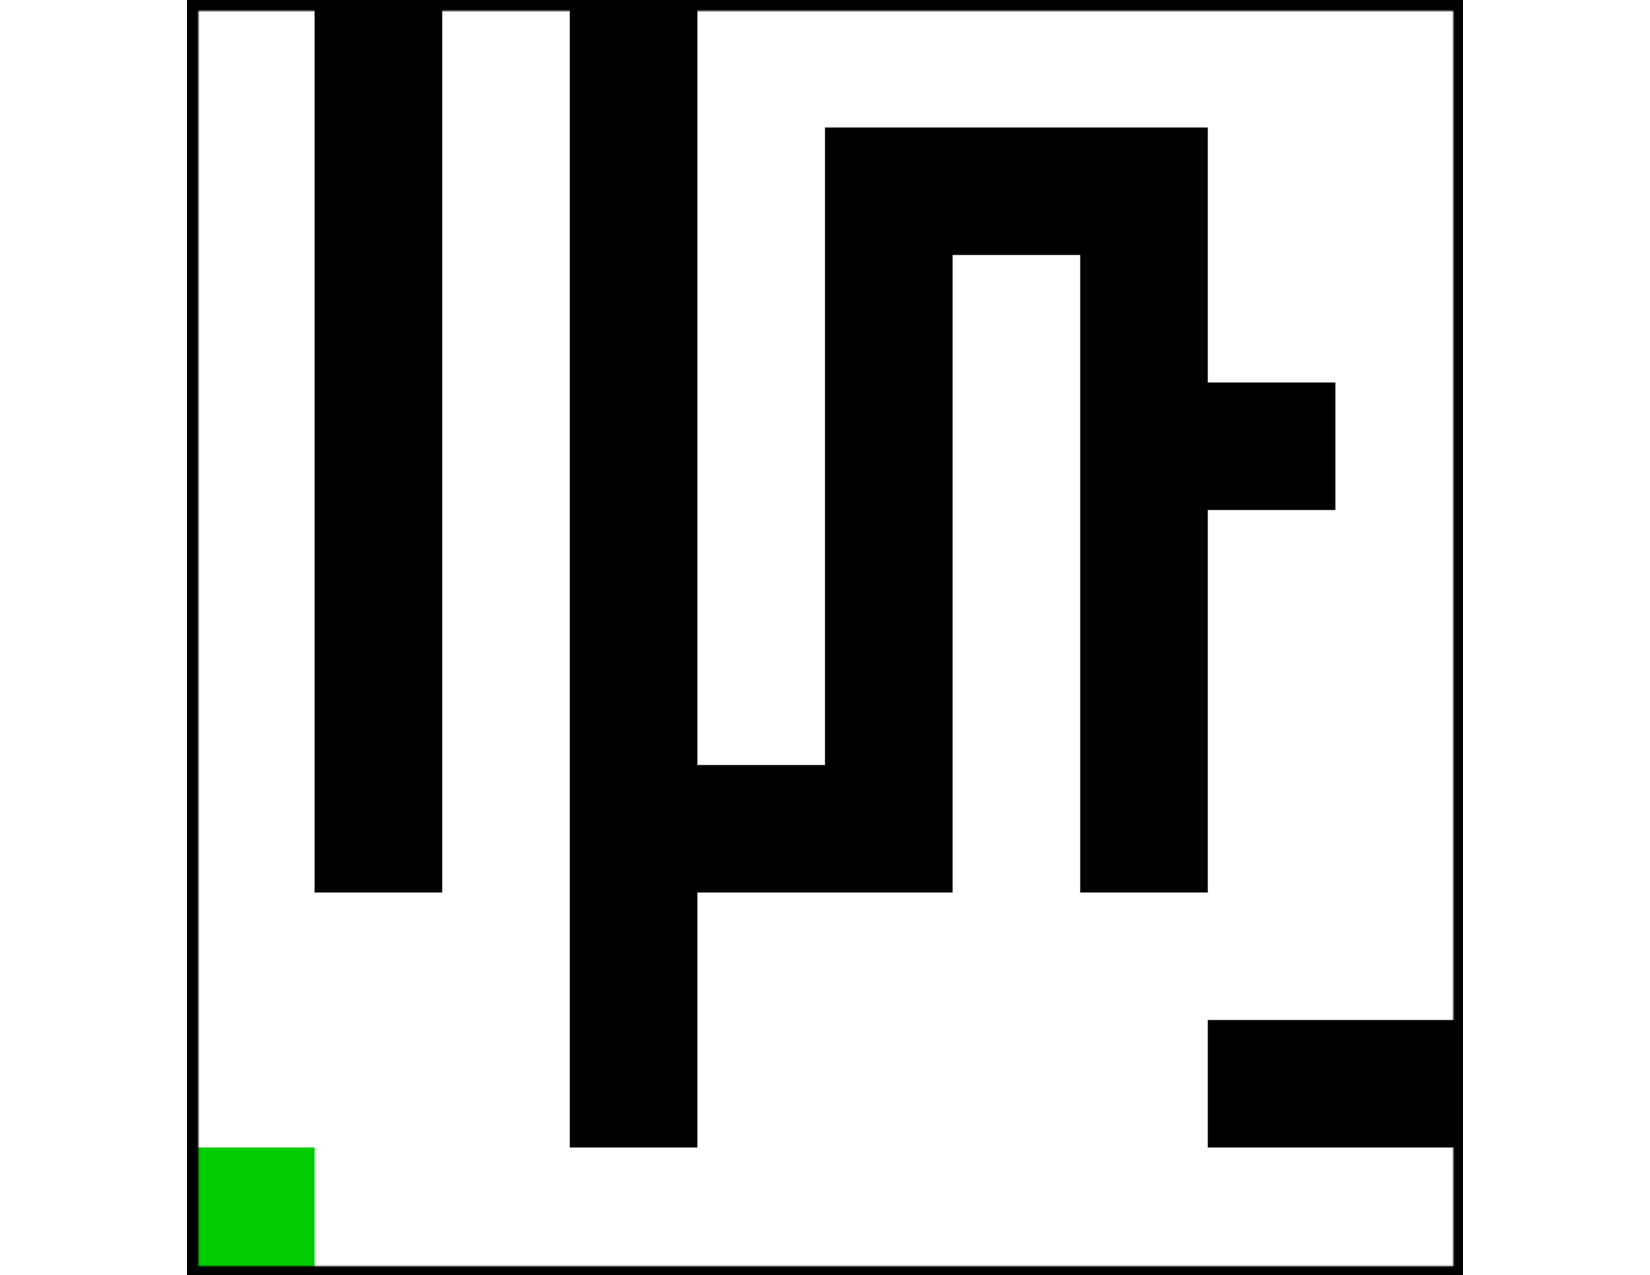
\includegraphics[width=\textwidth]{images/maze/maze12.pdf}
    \caption{}
  \end{subfigure}
  \begin{subfigure}[t]{0.18\textwidth}
    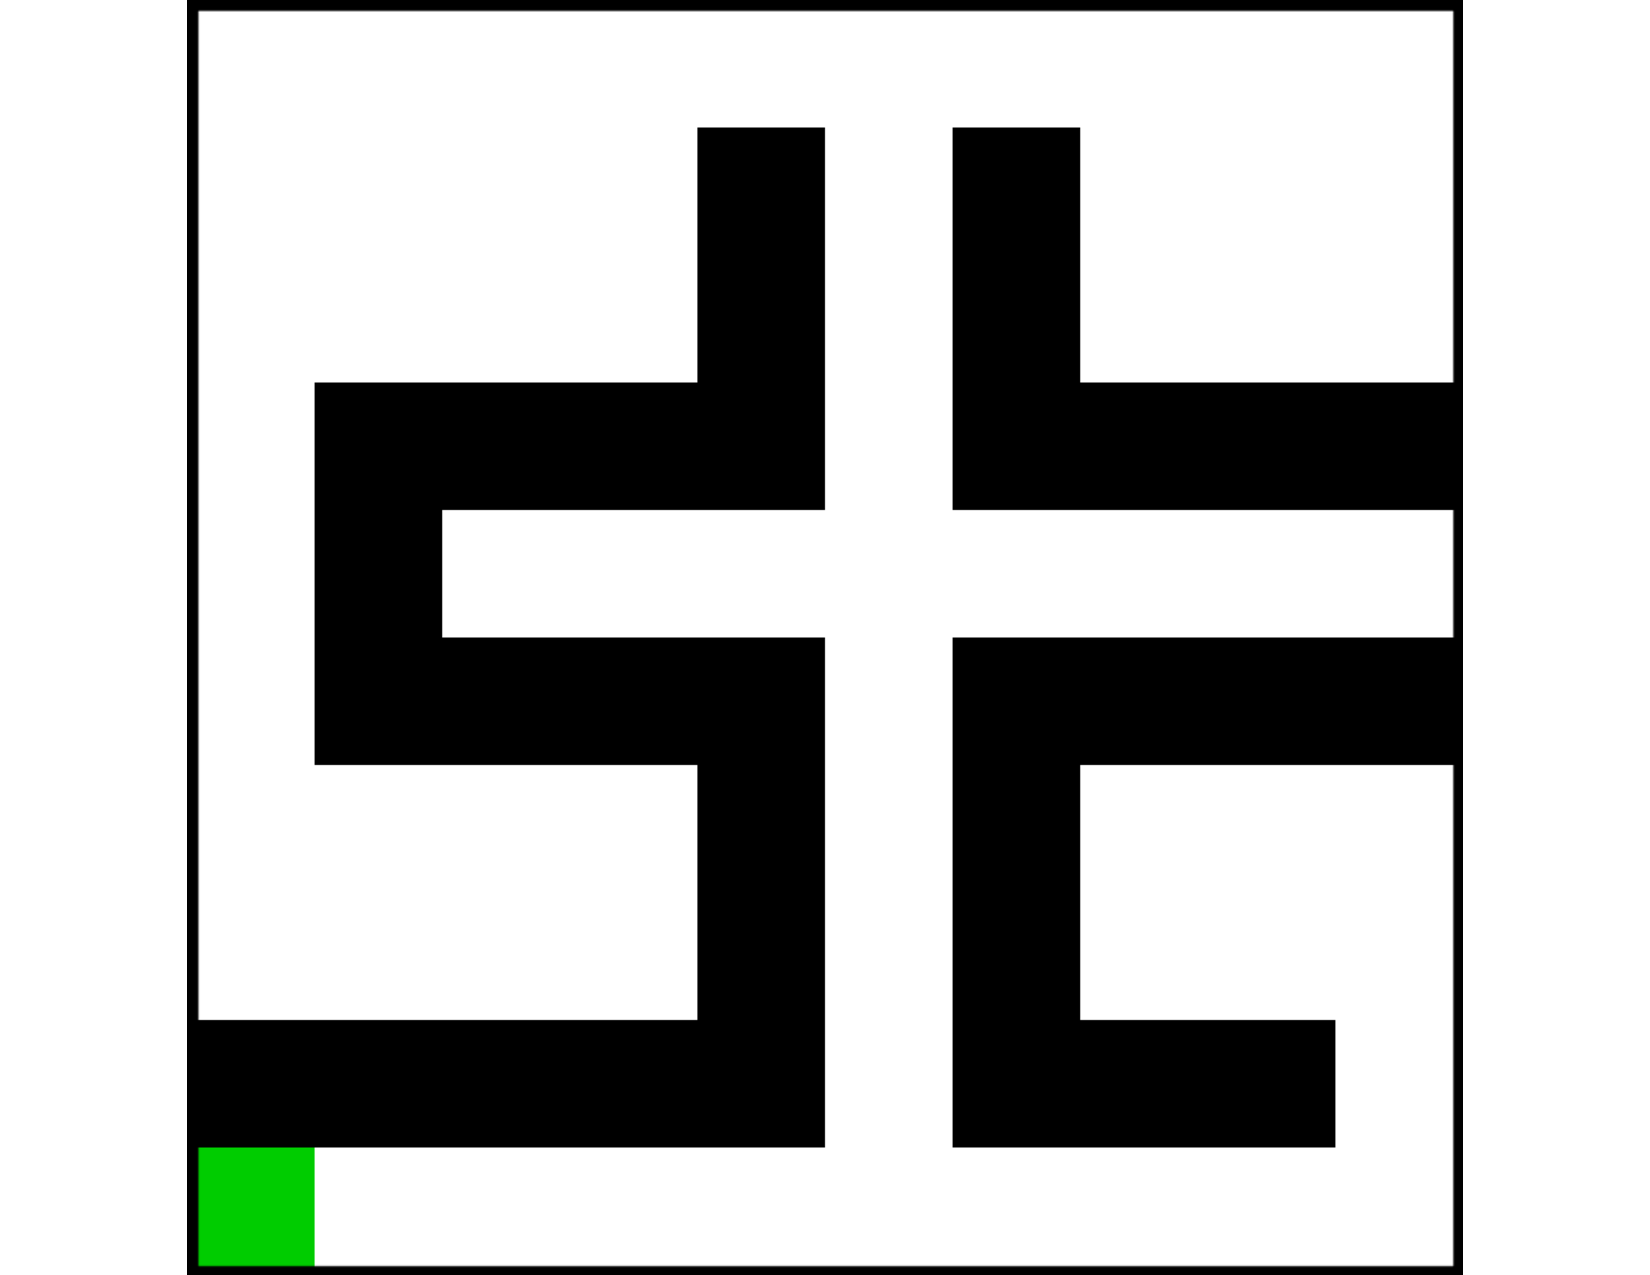
\includegraphics[width=\textwidth]{images/maze/maze13.pdf}
    \caption{}\label{fig:maze13}
  \end{subfigure}
  \begin{subfigure}[t]{0.18\textwidth}
    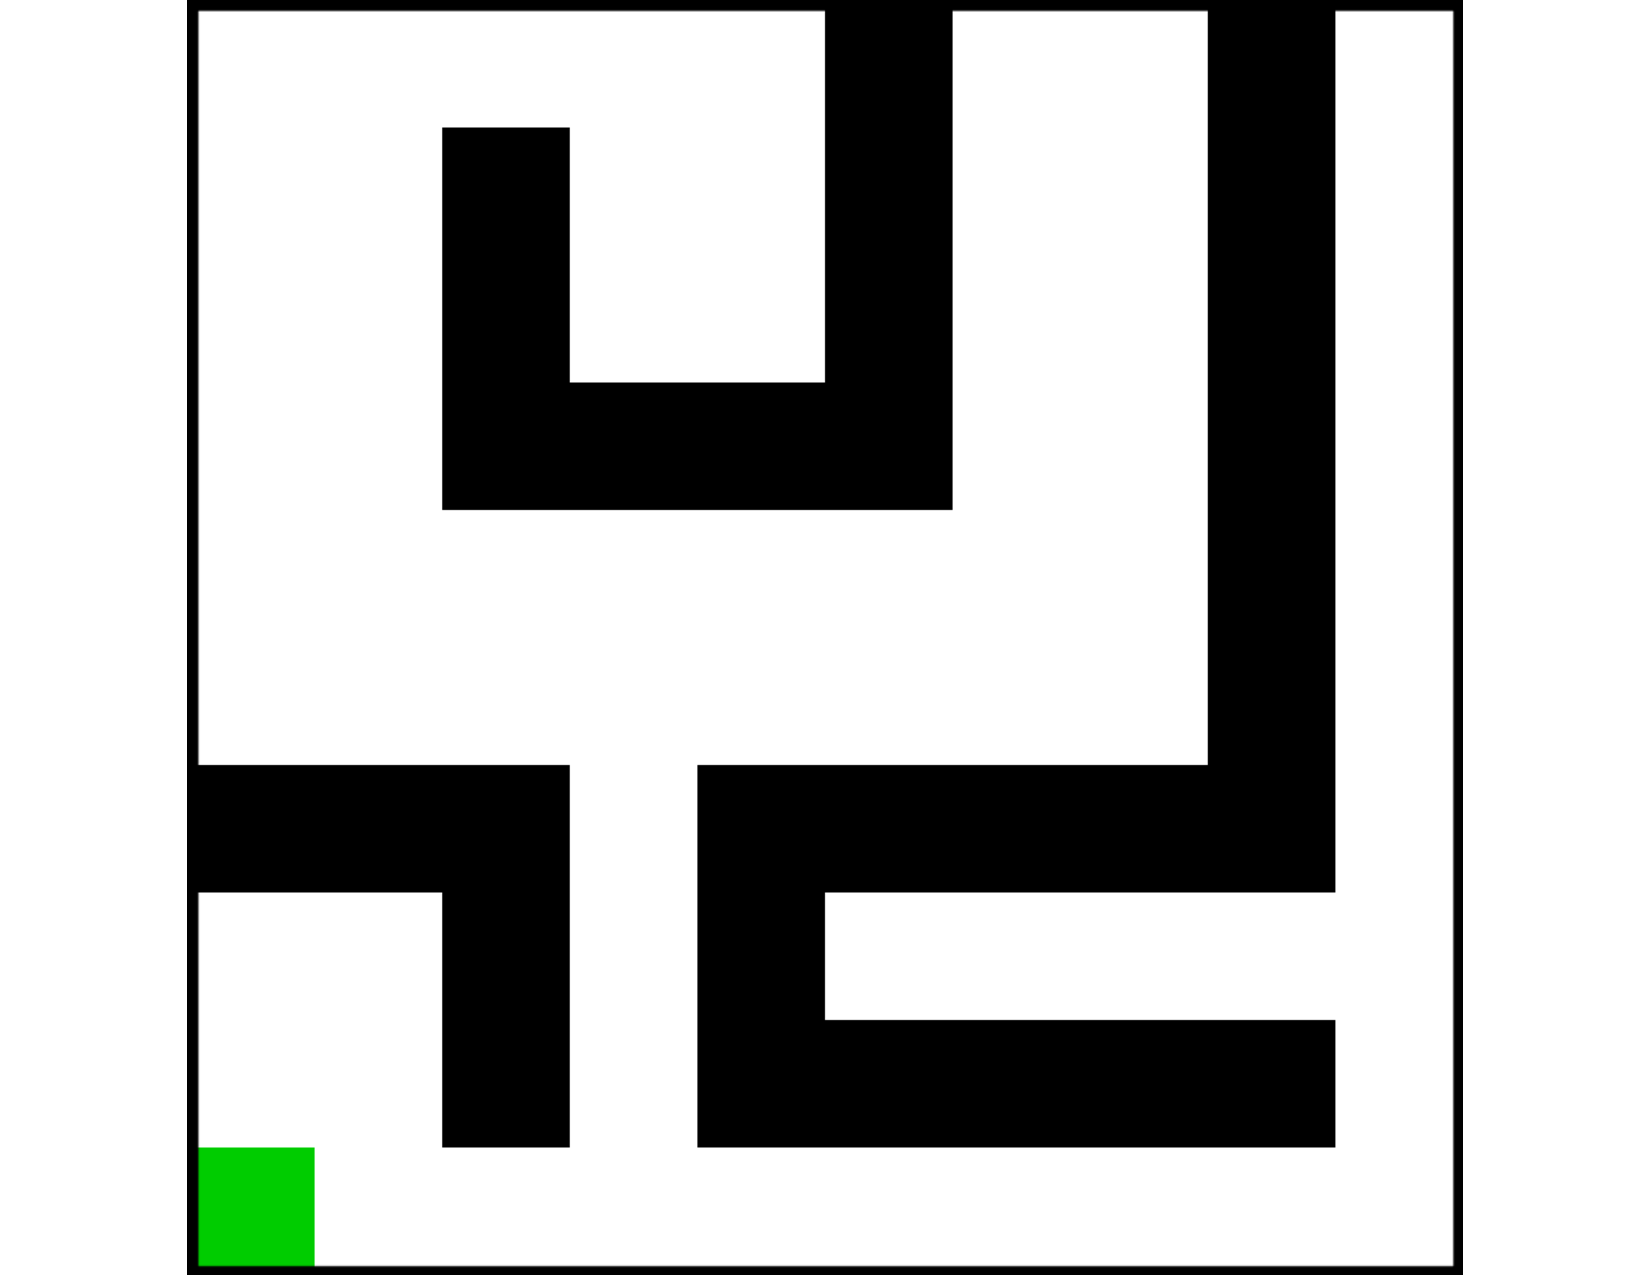
\includegraphics[width=\textwidth]{images/maze/maze14.pdf}
    \caption{}
  \end{subfigure}
  
  \begin{subfigure}[t]{0.18\textwidth}
    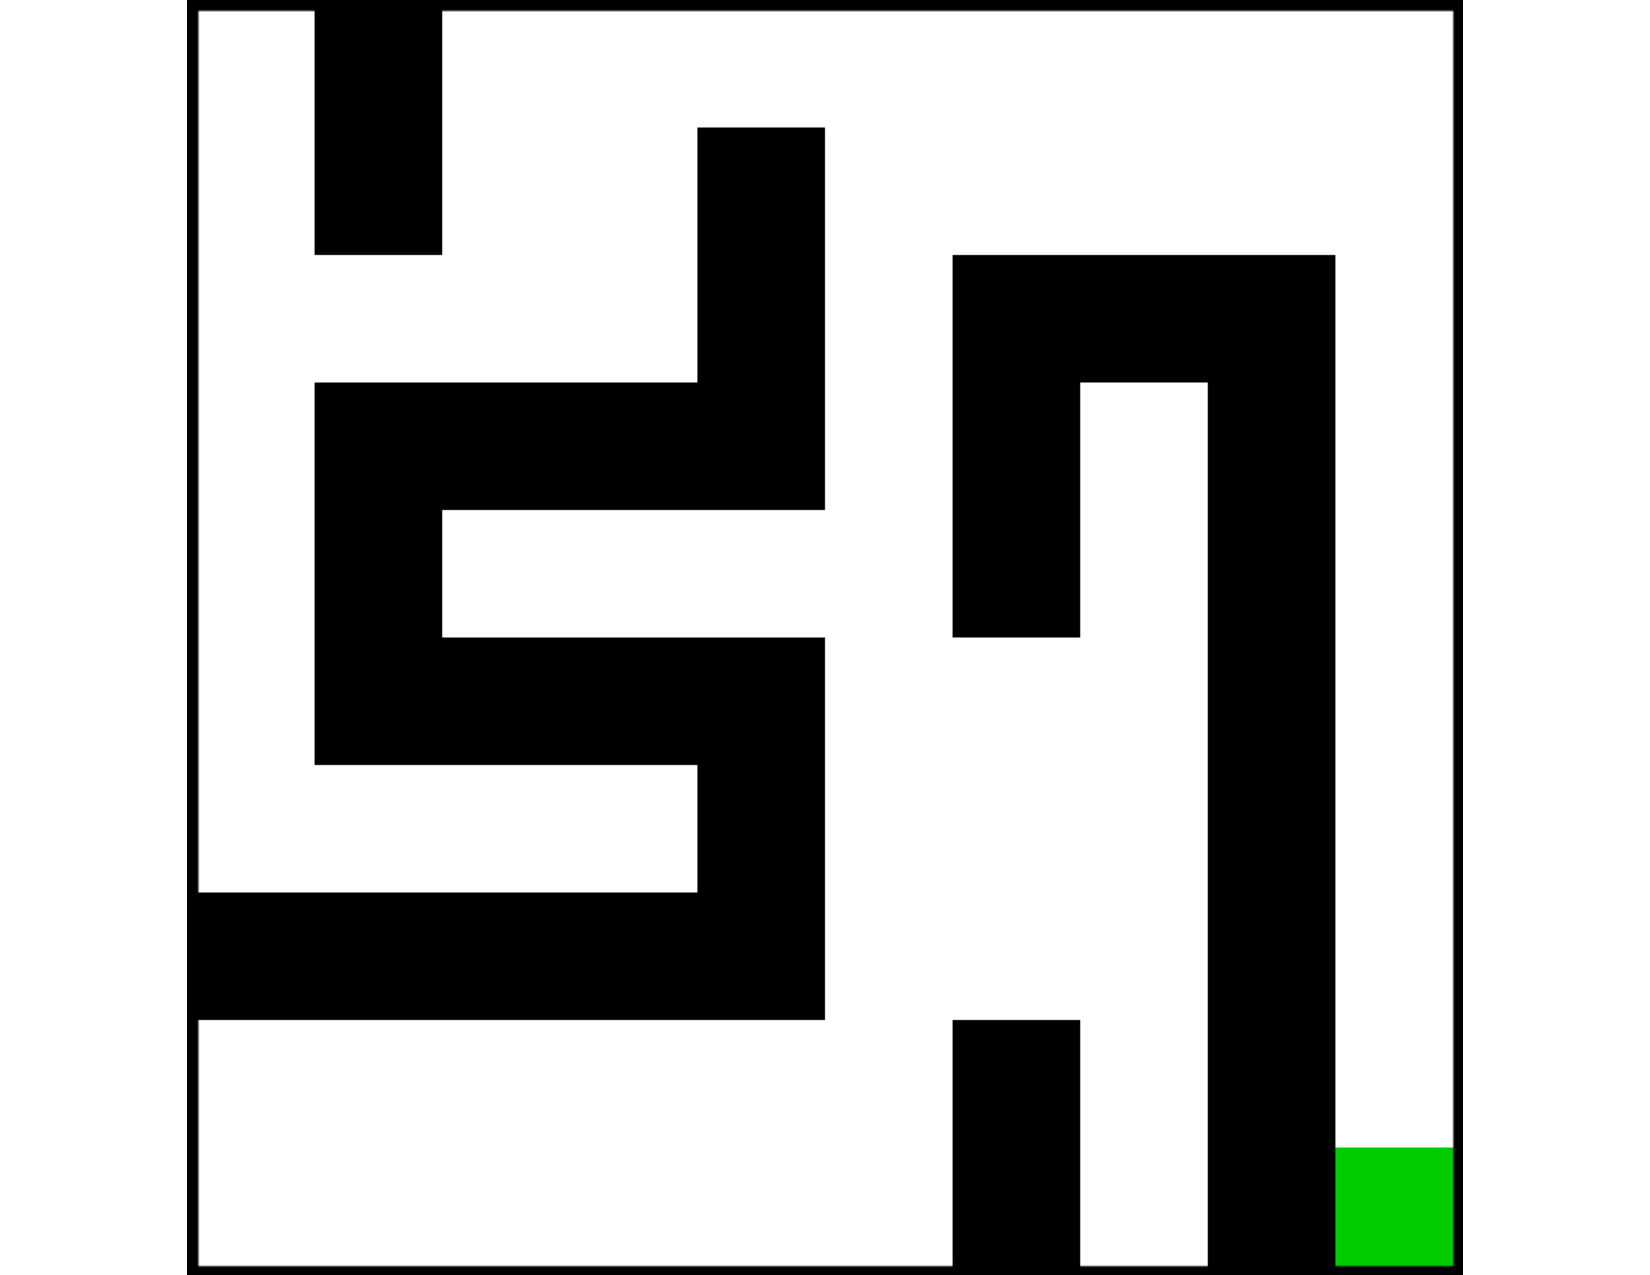
\includegraphics[width=\textwidth]{images/maze/maze15.pdf}
    \caption{}
  \end{subfigure}
  \begin{subfigure}[t]{0.18\textwidth}
    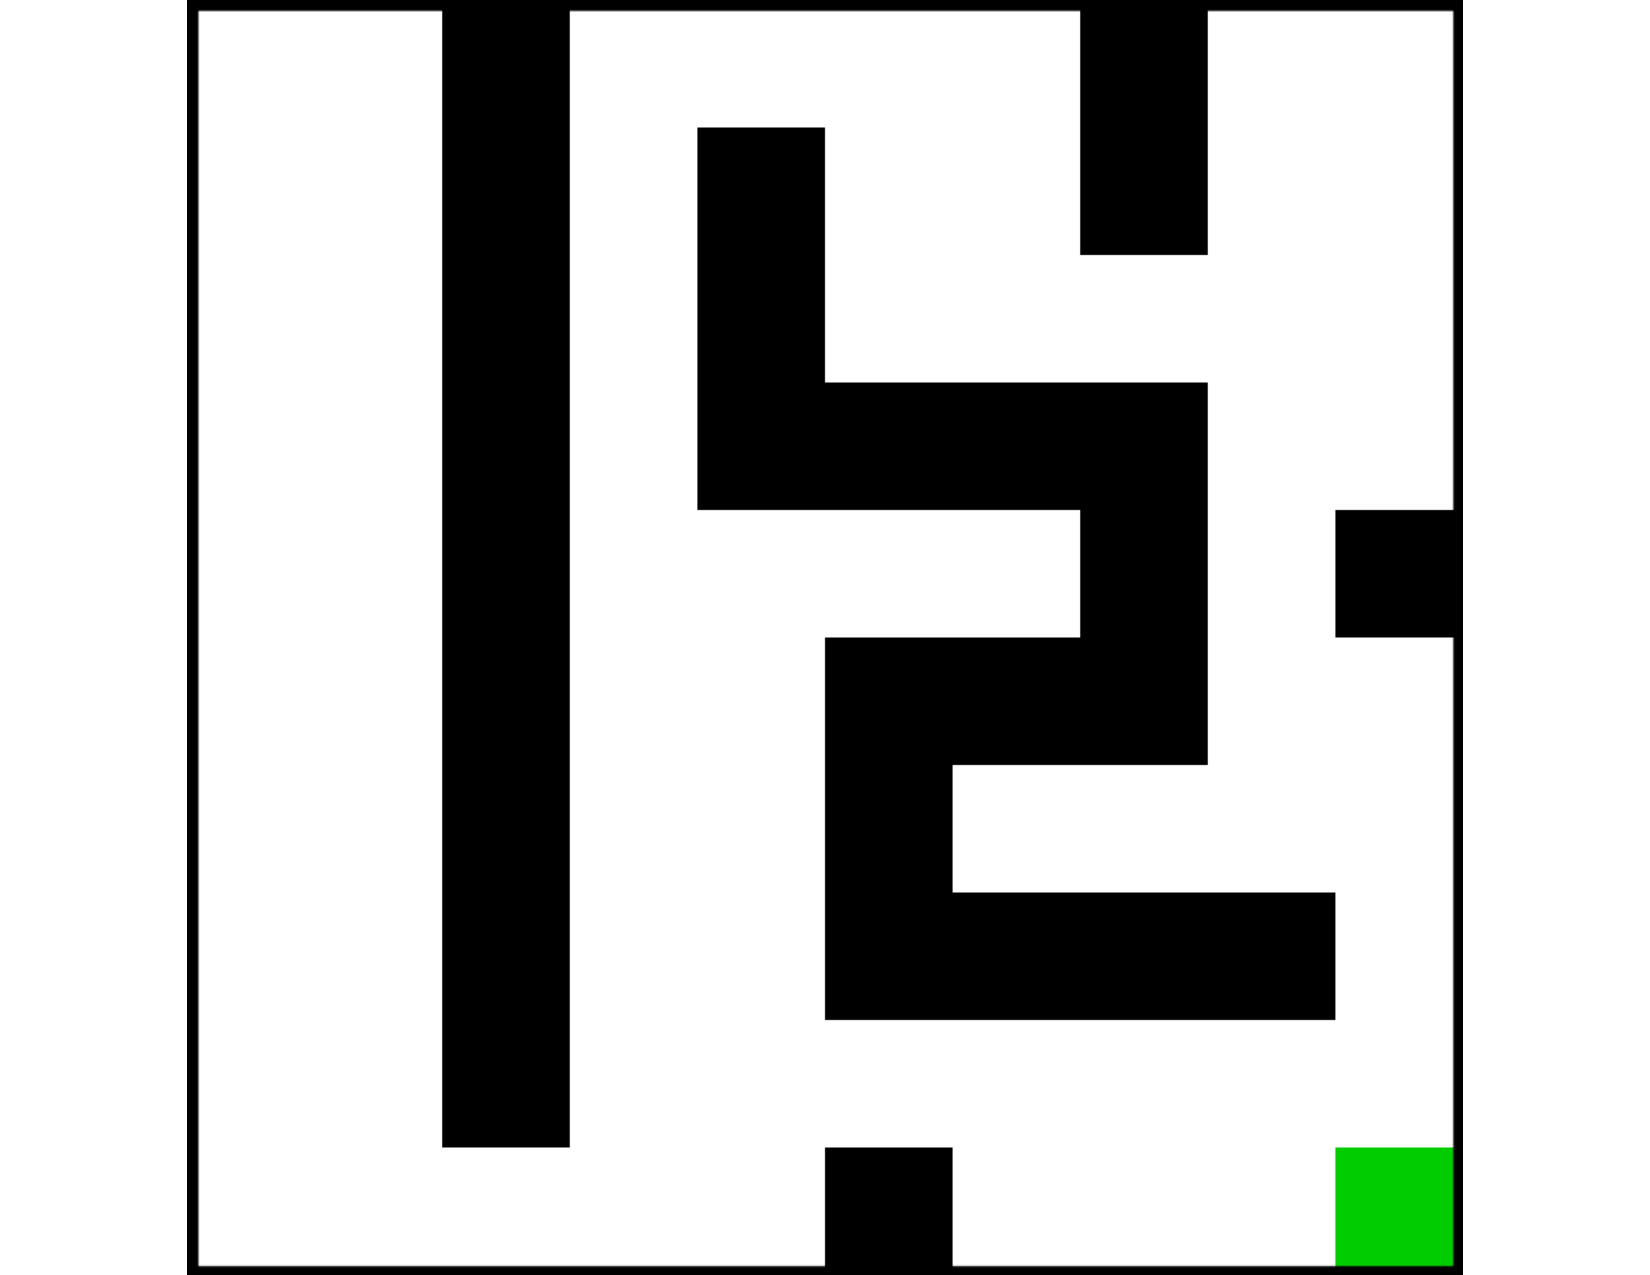
\includegraphics[width=\textwidth]{images/maze/maze16.pdf}
    \caption{}
  \end{subfigure}
  \begin{subfigure}[t]{0.18\textwidth}
    
\includegraphics[width=\textwidth]{images/maze/maze17.pdf}
    \caption{}
  \end{subfigure}
  \begin{subfigure}[t]{0.18\textwidth}
    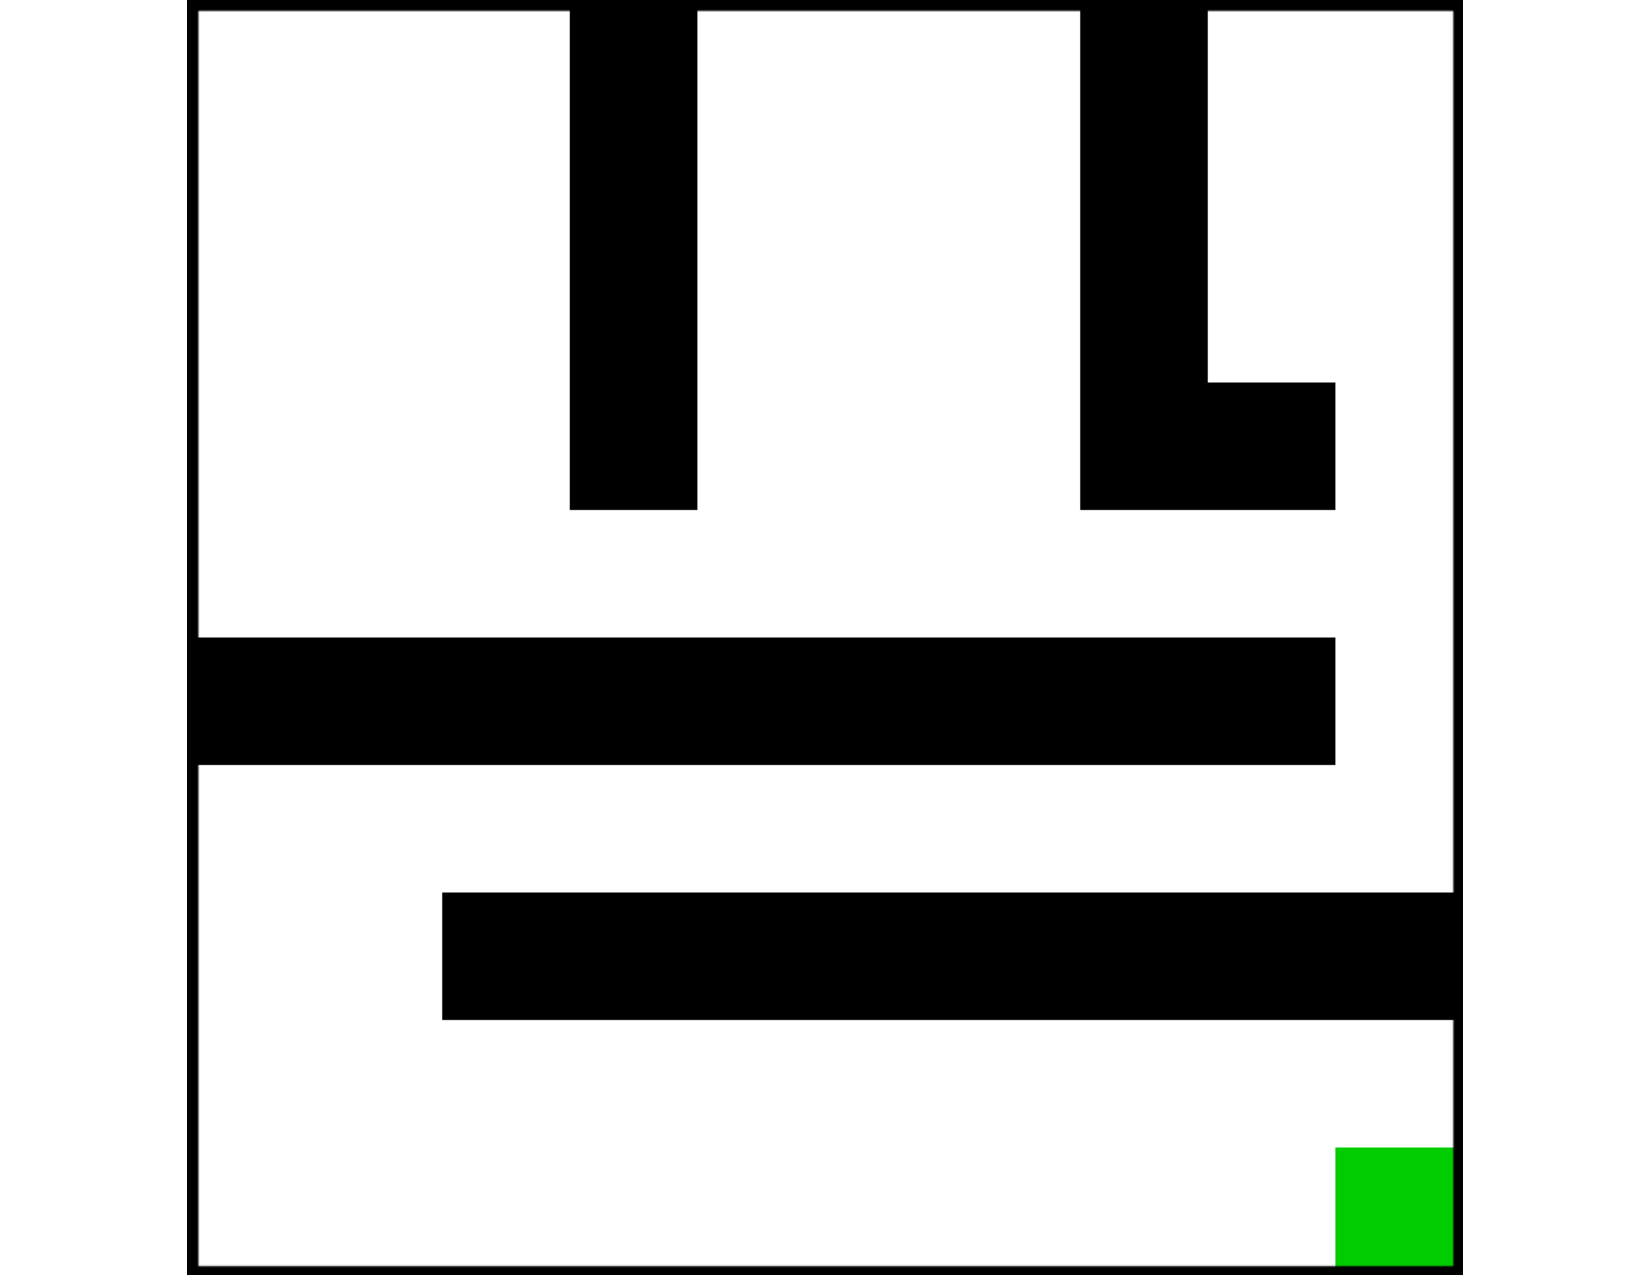
\includegraphics[width=\textwidth]{images/maze/maze18.pdf}
    \caption{}
  \end{subfigure}
  \begin{subfigure}[t]{0.18\textwidth}
    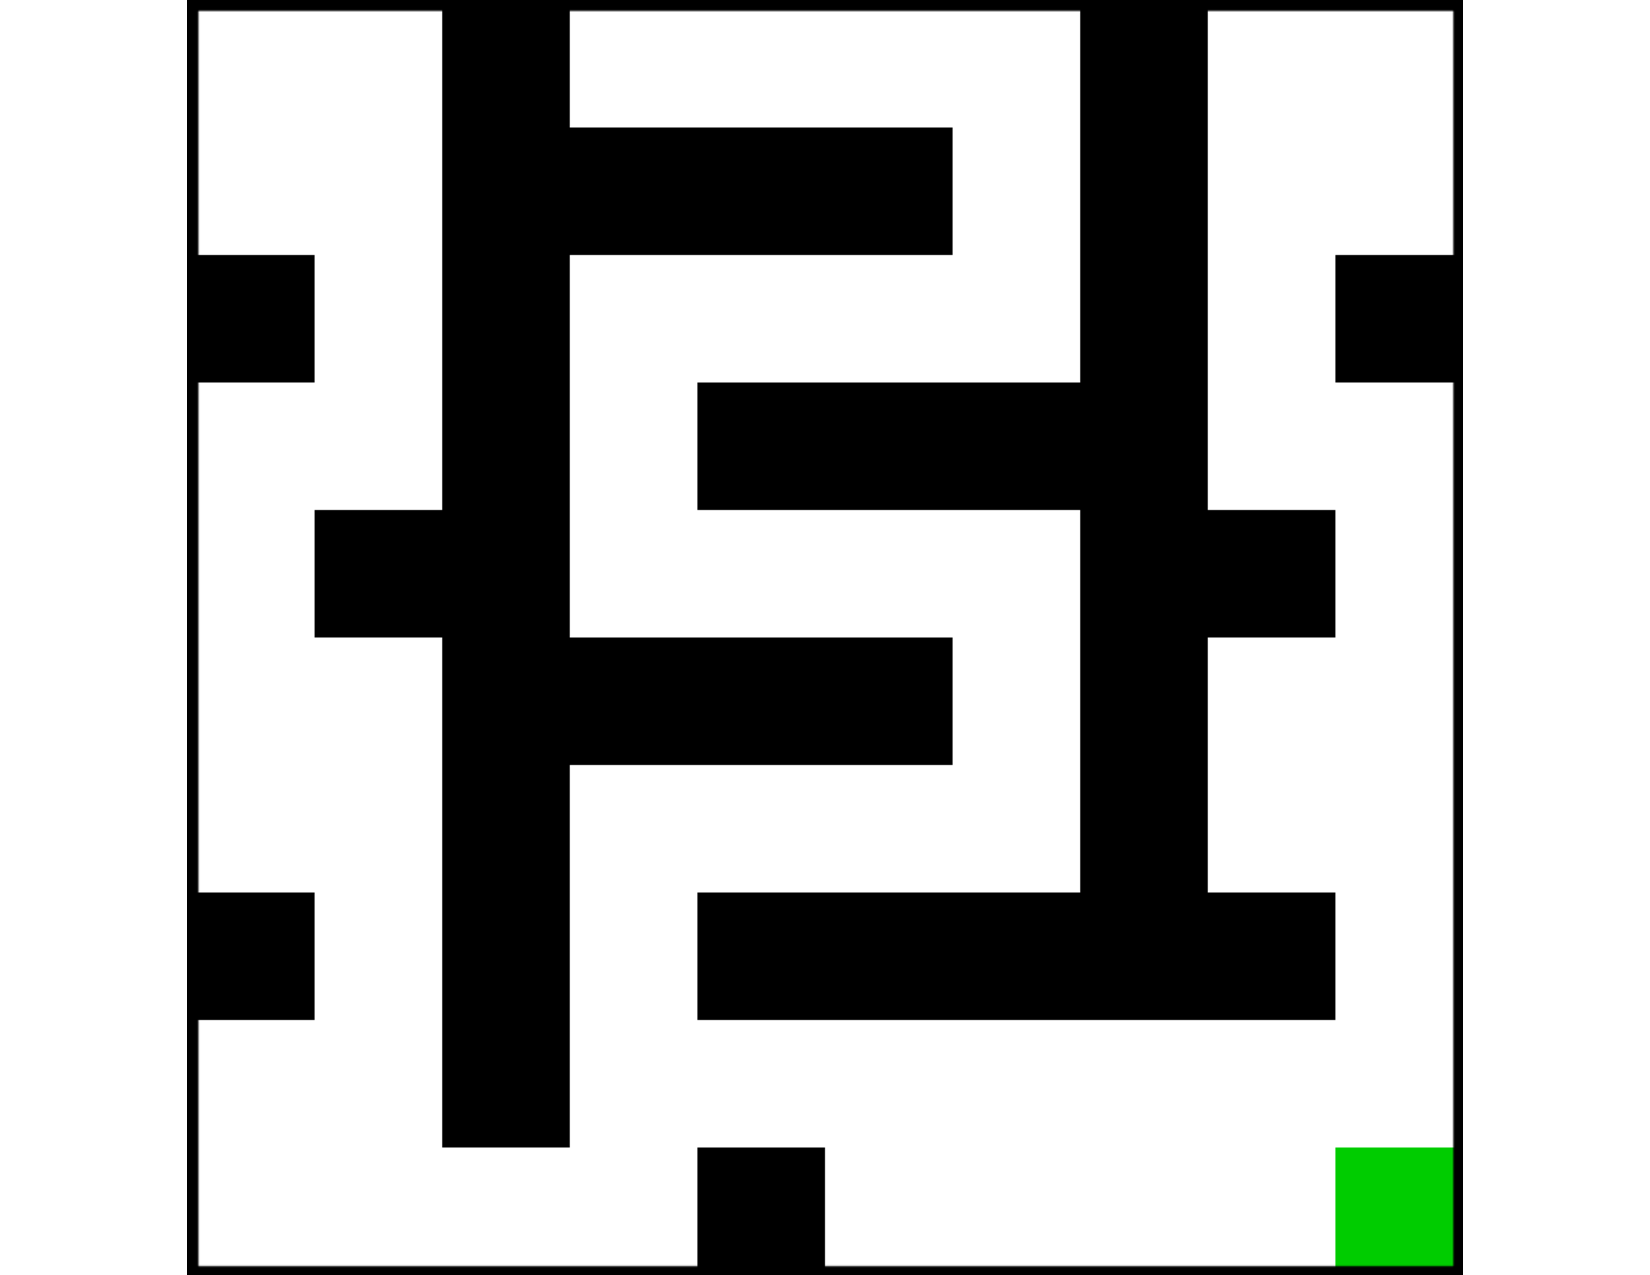
\includegraphics[width=\textwidth]{images/maze/maze19.pdf}
    \caption{}
  \end{subfigure}
  \caption{Set of mazes for the Maze Navigation task}
  \label{fig:mazes}
\end{figure*}

% Placer-holder to actual plots. Add analyses
\begin{figure*}[h]
	\begin{subfigure}[b]{0.45\textwidth}
    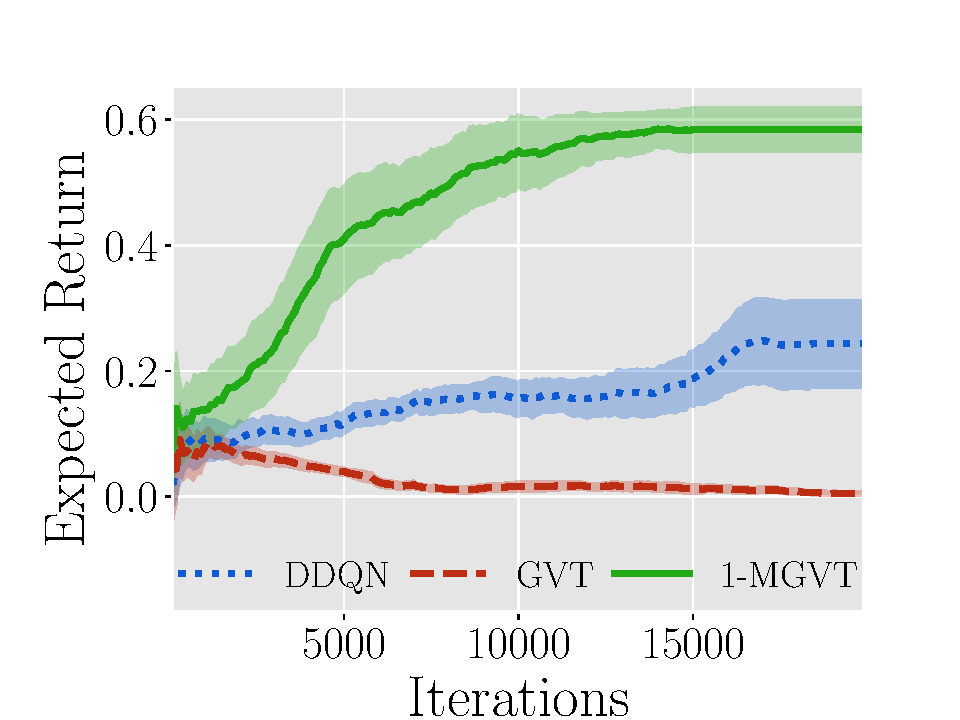
\includegraphics[trim=0.0cm 0cm 1.8cm 1.3cm,clip=true,height=4.5cm]{images/maze/lrev_maze0.pdf}
    \caption{Expected Return during learning}
  \end{subfigure}
  \begin{subfigure}[b]{0.45\textwidth}
    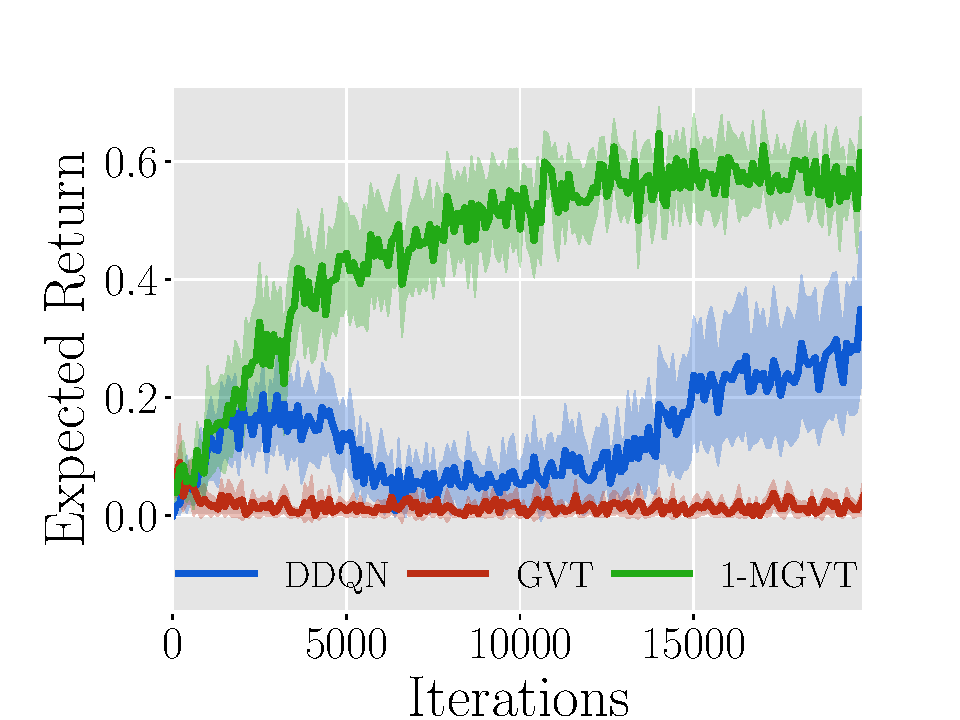
\includegraphics[trim=0.0cm 0cm 1.8cm 1.3cm,clip=true,height=4.5cm]{images/maze/erew_maze0.pdf}
    \caption{Expected Return w.r.t. greedy policy}
  \end{subfigure}
  \caption{Performance in Maze \ref{fig:maze0}}
  \label{fig:rew-maze0}
  
  \begin{subfigure}[b]{0.45\textwidth}
    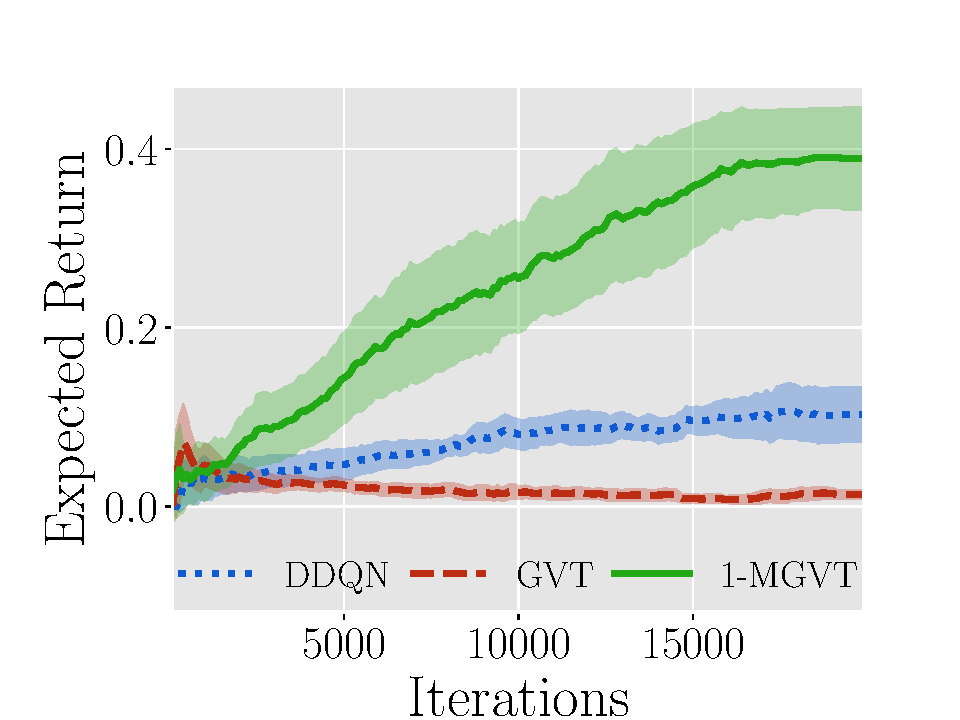
\includegraphics[trim=0.0cm 0cm 1.8cm 1.3cm,clip=true,height=4.5cm]{images/maze/lrev_maze6.pdf}
    \caption{Expected Return during learning}
  \end{subfigure}
  \begin{subfigure}[b]{0.45\textwidth}
    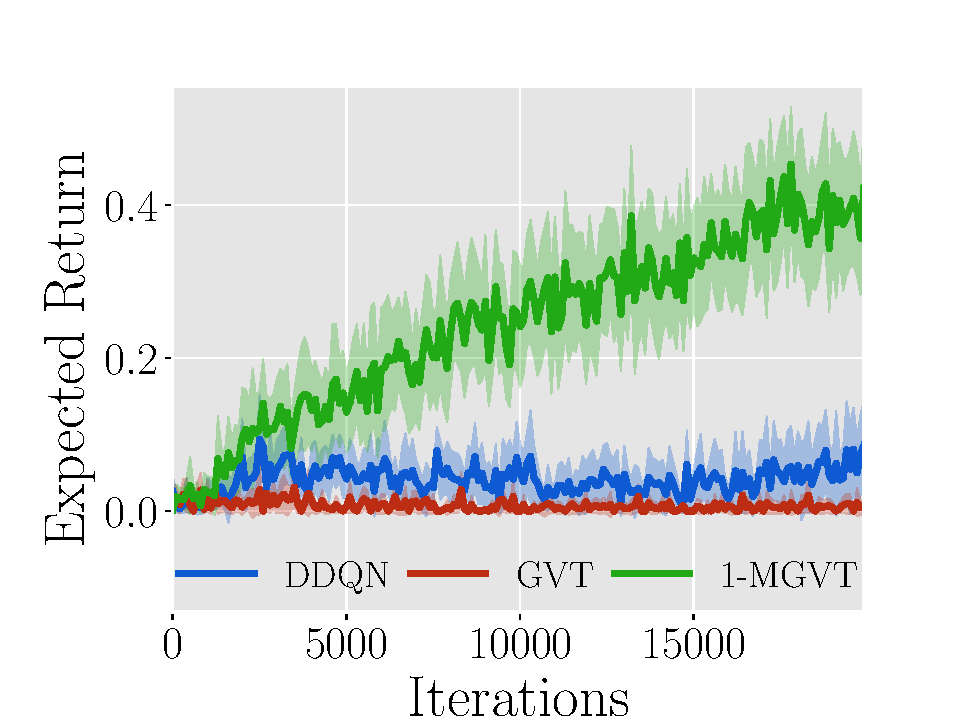
\includegraphics[trim=0.0cm 0cm 1.8cm 1.3cm,clip=true,height=4.5cm]{images/maze/erew_maze6.pdf}
    \caption{Expected Return w.r.t. greedy policy}
  \end{subfigure}
  \caption{Performance in Maze \ref{fig:maze6}}
  \label{fig:rew-maze6}
  
  \begin{subfigure}[b]{0.45\textwidth}
    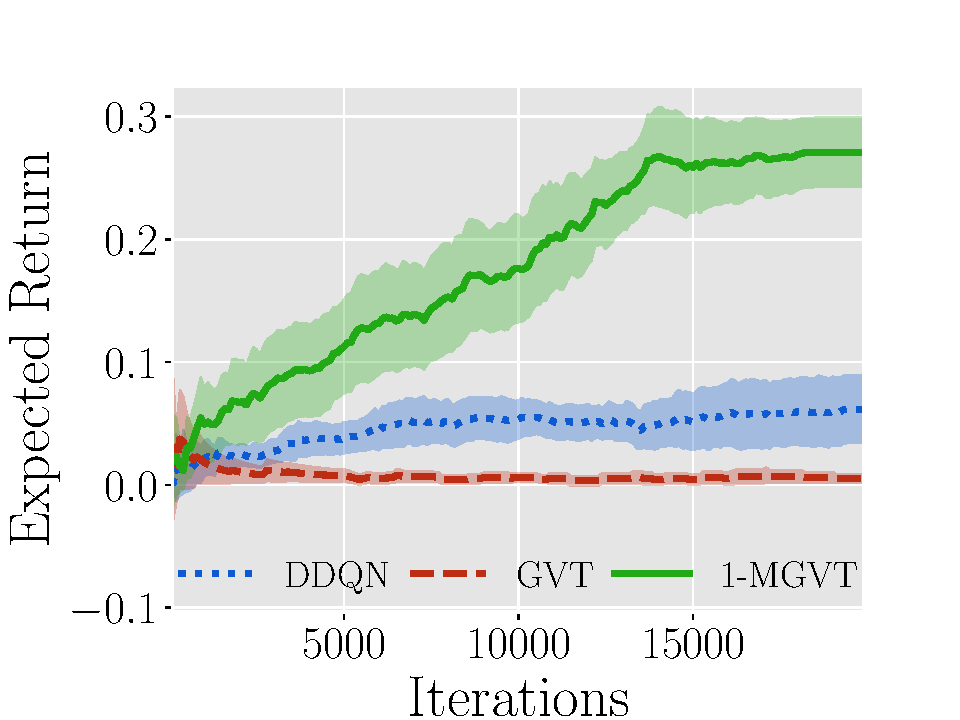
\includegraphics[trim=0.0cm 0cm 1.8cm 1.3cm,clip=true,height=4.5cm]{images/maze/lrev_maze13.pdf}
    \caption{Expected Return during learning}
  \end{subfigure}
  \begin{subfigure}[b]{0.45\textwidth}
    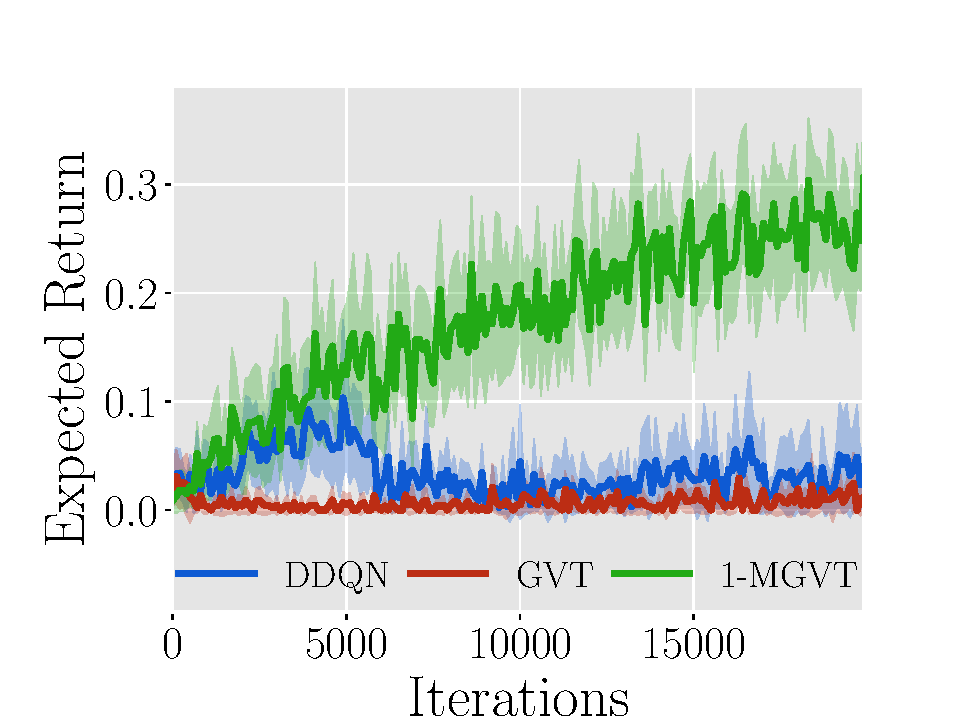
\includegraphics[trim=0.0cm 0cm 1.8cm 1.3cm,clip=true,height=4.5cm]{images/maze/erew_maze13.pdf}
    \caption{Expected Return w.r.t. greedy policy}
  \end{subfigure}
  \caption{Performance in Maze \ref{fig:maze13} }
  \label{fig:rew-maze13}
  
    \begin{subfigure}[b]{0.45\textwidth}
    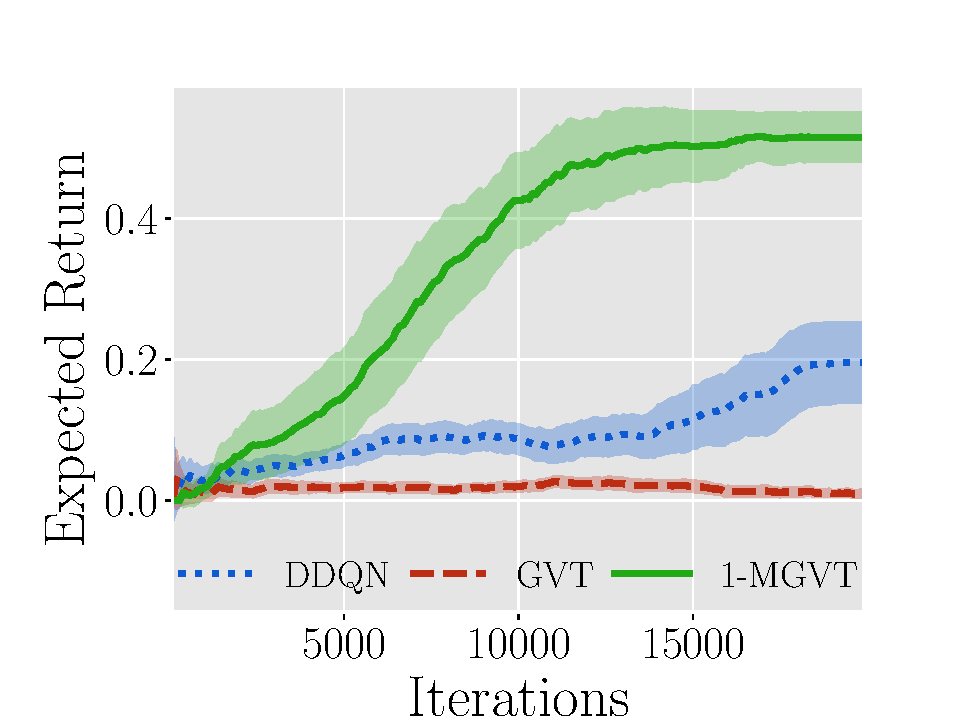
\includegraphics[trim=0.0cm 0cm 1.8cm 1.3cm,clip=true,height=4.5cm]{images/maze/lrev_maze8.pdf}
    \caption{Expected Return during learning}
  \end{subfigure}
  \begin{subfigure}[b]{0.45\textwidth}
    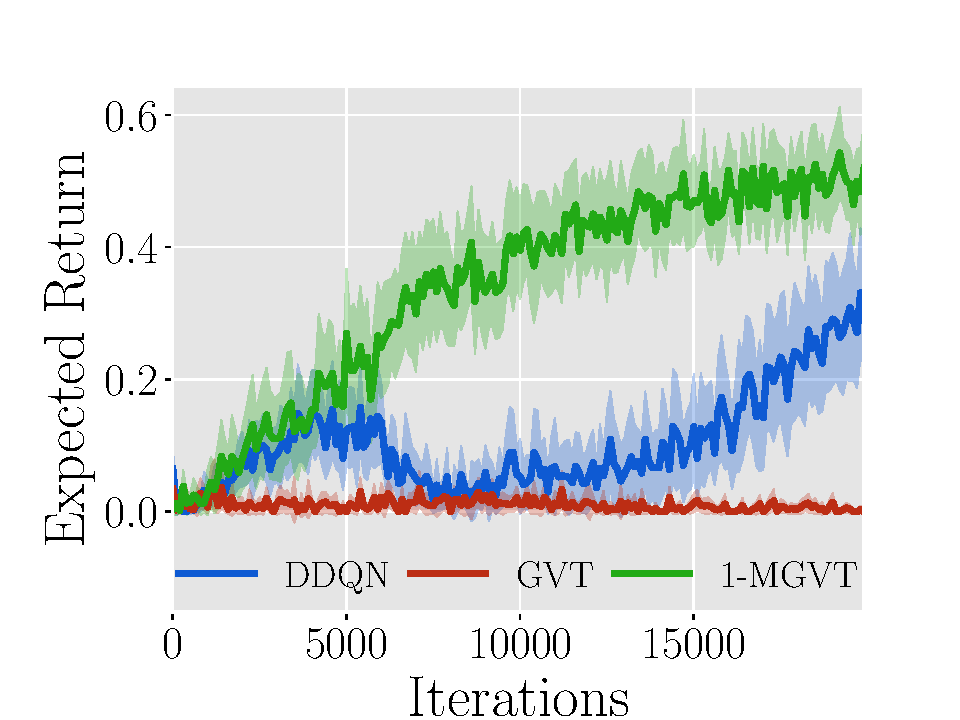
\includegraphics[trim=0.0cm 0cm 1.8cm 1.3cm,clip=true,height=4.5cm]{images/maze/erew_maze8.pdf}
    \caption{Expected Return w.r.t. greedy policy}
  \end{subfigure}
  \caption{Performance in Maze \ref{fig:maze8} }
  \label{fig:rew-maze8}
\end{figure*}

Hereafter, we present additional results of transferring from $5$ source tasks to the mazes shown in Figure \ref{fig:maze0}, Figure \ref{fig:maze6}, Figure \ref{fig:maze13}, and Figure \ref{fig:maze8} using both GVT and MGVT. We show both the greedy and online performances. All the curves result from averaging $20$ independent runs and randomly sampled sources.

In Figure \ref{fig:rew-maze0}, \ref{fig:rew-maze6}, \ref{fig:rew-maze13}, and \ref{fig:rew-maze8} we can appreciate that in this more complex transfer setting, MGVT is able to provide significant speed-up in a consistent manner in this subset of mazes. It is also noticeable the bad performance obtained with GVT in all cases. The Gaussian prior model clearly fails to capture enough information to transfer in this setting that result in a negative transfer effect.


\end{document}
